\documentclass[12pt,a4paper]{article}

% ================= PACKAGES =================
\usepackage[utf8]{inputenc}
\usepackage[T5]{fontenc}
\usepackage[vietnamese]{babel}
\usepackage{amsmath,amssymb,amsfonts}
\usepackage{geometry}
\geometry{left=3.0cm,right=2.0cm,top=2.5cm,bottom=2.5cm}
\usepackage{setspace}
\onehalfspacing
\setlength{\parindent}{1.27cm}
\setlength{\parskip}{6pt}
\usepackage{graphicx}
\usepackage{booktabs}
\usepackage{longtable}
\usepackage{array}
\usepackage{multirow}
\usepackage{float}
\usepackage{caption}
\usepackage{subcaption}
\usepackage{xcolor}
\usepackage{listings}
\usepackage{tikz}
\usetikzlibrary{shapes.geometric, arrows.meta, positioning}
\usepackage{fancyhdr}
\usepackage{hyperref}

\hypersetup{
    colorlinks=true,
    linkcolor=blue!70!black,
    citecolor=blue!70!black,
    urlcolor=blue!70!black,
    pdftitle={Bao Cao Bai Tap Lon Nhap Mon Hoc May - De Tai 13},
}

% ================= CODE LISTING STYLE =================
\definecolor{codebg}{rgb}{0.97,0.97,0.98}
\definecolor{codegreen}{rgb}{0.1,0.5,0.2}
\definecolor{codegray}{rgb}{0.45,0.45,0.45}
\definecolor{codeblue}{rgb}{0.1,0.2,0.7}

\lstdefinestyle{pythonstyle}{
    language=Python,
    backgroundcolor=\color{codebg},
    commentstyle=\color{codegreen}\itshape,
    keywordstyle=\color{codeblue}\bfseries,
    numberstyle=\tiny\color{codegray},
    stringstyle=\color{red!70!black},
    basicstyle=\ttfamily\footnotesize,
    breakatwhitespace=false,
    breaklines=true,
    captionpos=b,
    keepspaces=true,
    numbers=left,
    numbersep=6pt,
    showspaces=false,
    showstringspaces=false,
    showtabs=false,
    tabsize=4,
    frame=single,
    rulecolor=\color{black!25},
}
\lstset{style=pythonstyle}

% ================= HEADER / FOOTER =================
\pagestyle{fancy}
\fancyhf{}
\fancyhead[L]{\small Học phần: Nhập môn Học máy (FIT4013)}
\fancyhead[R]{\small Đề tài 13: Dự đoán nhân viên nghỉ việc}
\fancyfoot[C]{\thepage}
\renewcommand{\headrulewidth}{0.4pt}

\begin{document}

% ================= TITLE PAGE (CHUẨN ĐẠI HỌC ĐẠI NAM) =================
\begin{titlepage}
    \begin{tikzpicture}[remember picture, overlay]
        \draw[line width=2pt]
            ([xshift=1.8cm,yshift=-1.5cm]current page.north west)
            rectangle
            ([xshift=-1.5cm,yshift=1.5cm]current page.south east);
        \draw[line width=0.6pt]
            ([xshift=1.95cm,yshift=-1.65cm]current page.north west)
            rectangle
            ([xshift=-1.65cm,yshift=1.65cm]current page.south east);
    \end{tikzpicture}

    \centering
    \vspace*{0.2cm}
    {\large \textbf{BỘ GIÁO DỤC VÀ ĐÀO TẠO}}\\
    {\large \textbf{TRƯỜNG ĐẠI HỌC ĐẠI NAM}}\\
    \rule{4.6cm}{0.6pt}\\[0.5cm]

    
\includegraphics[width=3.6cm]{figures/logo_dnu.png}\\[0.8cm]

    {\huge \textbf{BÀI TẬP LỚN}}\\[0.5cm]
    {\large \textbf{TÊN HỌC PHẦN: Nhập môn Học máy (FIT4013)}}\\[0.3cm]
    {\large \textbf{ĐỀ TÀI: Dự đoán nhân viên có khả năng nghỉ việc}}\\
    {\large \textbf{(Employee Attrition Prediction)}}\\[1.2cm]

    \begin{flushleft}
        \hspace{1.0cm} {\large \textbf{Giáo viên hướng dẫn:} ThS. Lê Thị Thùy Trang}\\[0.35cm]
        \hspace{1.0cm} {\large \textbf{Sinh viên thực hiện:}}
    \end{flushleft}
    \vspace{0.15cm}

    \begin{table}[H]
    \centering
    \renewcommand{\arraystretch}{1.25}
    \begin{tabular}{|c|c|l|c|}
    \hline
    \textbf{Stt} & \textbf{Mã sv} & \textbf{Họ và tên} & \textbf{Lớp} \\
    \hline
    1 & 1871020003 & Nguyễn Văn An & CNTT 18-05 \\
    \hline
    2 & 1871020047 & Nguyễn Việt Anh & CNTT 18-05 \\
    \hline
    3 & 1871020307 & Lê Đình Huy & CNTT 18-05 \\
    \hline
    4 & 1871020639 & Đào Thị Tươi (Trưởng nhóm) & CNTT 18-05 \\
    \hline
    \end{tabular}
    \end{table}

    \vfill
    {\large \textbf{Hà Nội, năm 2026}}
    \vspace*{0.3cm}
\end{titlepage}

% ================= TITLE PAGE 2 (PHIẾU CHẤM ĐIỂM) =================
\begin{titlepage}
    \begin{tikzpicture}[remember picture, overlay]
        \draw[line width=2pt]
            ([xshift=1.8cm,yshift=-1.5cm]current page.north west)
            rectangle
            ([xshift=-1.5cm,yshift=1.5cm]current page.south east);
        \draw[line width=0.6pt]
            ([xshift=1.95cm,yshift=-1.65cm]current page.north west)
            rectangle
            ([xshift=-1.65cm,yshift=1.65cm]current page.south east);
    \end{tikzpicture}

    \centering
    \vspace*{0.2cm}
    {\large \textbf{BỘ GIÁO DỤC VÀ ĐÀO TẠO}}\\
    {\large \textbf{TRƯỜNG ĐẠI HỌC ĐẠI NAM}}\\
    \rule{4.6cm}{0.6pt}\\[0.5cm]

    
\includegraphics[width=3.6cm]{figures/logo_dnu.png}\\[0.8cm]

    {\huge \textbf{BÀI TẬP LỚN}}\\[0.5cm]
    {\large \textbf{TÊN HỌC PHẦN: Nhập môn Học máy (FIT4013)}}\\[0.3cm]
    {\large \textbf{ĐỀ TÀI: Dự đoán nhân viên có khả năng nghỉ việc}}\\[1.0cm]

    \begin{flushright}
        {\large \textbf{CÁN BỘ CHẤM THI}}\hspace*{1.0cm}
    \end{flushright}
    \vspace{0.3cm}

    \begin{table}[H]
    \centering
    \renewcommand{\arraystretch}{1.3}
    \begin{tabular}{|c|c|l|c|c|c|}
    \hline
    \multirow{2}{*}{\textbf{STT}} & \multirow{2}{*}{\textbf{Mã Sinh Viên}} & \multirow{2}{*}{\textbf{Họ và Tên}} & \multirow{2}{*}{\textbf{Ngày Sinh}} & \multicolumn{2}{c|}{\textbf{Điểm}} \\
    \cline{5-6}
     & & & & \textbf{Bằng Số} & \textbf{Bằng Chữ} \\
    \hline
    1 & 1871020003 & Nguyễn Văn An & 15/02/2006 & & \\
    \hline
    2 & 1871020047 & Nguyễn Việt Anh & 20/05/2006 & & \\
    \hline
    3 & 1871020307 & Lê Đình Huy & 09/05/2006 & & \\
    \hline
    4 & 1871020639 & Đào Thị Tươi & 06/08/2006 & & \\
    \hline
    \end{tabular}
    \end{table}

    \vfill
    {\large \textbf{Hà Nội, năm 2026}}
    \vspace*{0.3cm}
\end{titlepage}


% ================= BẢNG PHÂN CÔNG NHIỆM VỤ RIÊNG =================
\newpage
\section*{BẢNG PHÂN CÔNG NHIỆM VỤ THỰC HIỆN (NHÓM 7)}
\addcontentsline{toc}{section}{Bảng phân công nhiệm vụ thực hiện (Nhóm 7)}

Nhóm 7 gồm bốn thành viên cùng phối hợp thực hiện Đề tài 13 dưới sự điều phối chung của trưởng nhóm Đào Thị Tươi. Toàn bộ thành viên đều tham gia thảo luận phương án kỹ thuật, kiểm tra chéo mã nguồn và thống nhất số liệu báo cáo trước khi hoàn thiện. Bảng dưới đây trình bày chi tiết nhiệm vụ phụ trách chính và tỷ lệ đóng góp của từng thành viên.

\begin{table}[H]
\centering
\caption{Bảng phân công nhiệm vụ các thành viên Nhóm 7.}
\label{tab:team_assignment_front}
\small
\renewcommand{\arraystretch}{1.3}
\begin{tabular}{|c|l|c|c|p{6.0cm}|c|c|}
\hline
\textbf{STT} & \textbf{Họ và tên} & \textbf{Mã SV} & \textbf{Vai trò} & \textbf{Nhiệm vụ phụ trách chính} & \textbf{Đóng góp} & \textbf{Đánh giá} \\
\hline
1 & Đào Thị Tươi & 1871020639 & Trưởng nhóm & Điều phối tiến độ chung; lập kế hoạch nghiên cứu; tiền xử lý Luồng A; huấn luyện mô hình Baseline, tinh chỉnh siêu tham số bằng GridSearchCV cho K-NN, Gaussian NB, Decision Tree; phân tích ma trận nhầm lẫn và biên soạn Chương 4; tổng hợp và chuẩn hóa báo cáo toàn diện. & 25\% & Xuất sắc \\
\hline
2 & Nguyễn Văn An & 1871020003 & Thành viên & Nghiên cứu bối cảnh quản trị nhân sự; thu thập và làm sạch sơ bộ dữ liệu; phân tích khám phá dữ liệu chuyên sâu (EDA 35 thuộc tính); kiểm định thống kê giả thuyết phi tham số Mann-Whitney U và Chi-square; phân tích tương quan và đa cộng tuyến VIF; biên soạn Chương 1. & 25\% & Xuất sắc \\
\hline
3 & Nguyễn Việt Anh & 1871020047 & Thành viên & Thiết kế kiến trúc Pipeline chống rò rỉ dữ liệu; hiện thực hóa lớp biến đổi tùy chỉnh HRFeatureEngineer tạo 7 đặc trưng miền nghiệp vụ HR; áp dụng biến đổi log1p và chuẩn hóa RobustScaler; tích hợp thuật toán chọn lọc đặc trưng ANOVA F-test; kiểm thử đơn vị unittest; biên soạn Chương 2 và Chương 3. & 25\% & Xuất sắc \\
\hline
4 & Lê Đình Huy & 1871020307 & Thành viên & Phát triển mô hình mở rộng Random Forest; phân tích lỗi chuyên sâu (False Negatives và False Positives); tối ưu hóa ngưỡng xác suất quyết định; xây dựng mô hình định lượng hiệu quả kinh tế nhân sự HR ROI đa kịch bản; thiết kế và hoàn thiện ứng dụng Web Demo Streamlit 3 phân hệ; biên soạn Chương 5 và Chương 6. & 25\% & Xuất sắc \\
\hline
\end{tabular}
\end{table}

\vspace{0.8cm}
\begin{flushright}
\textit{Hà Nội, ngày 15 tháng 11 năm 2026}\\[0.2cm]
\textbf{Trưởng nhóm xác nhận}\\[1.5cm]
\textbf{Đào Thị Tươi}
\end{flushright}

\newpage
\section*{TÓM TẮT ĐỀ TÀI}
\addcontentsline{toc}{section}{Tóm tắt đề tài}

Báo cáo nghiên cứu khoa học này trình bày toàn diện quy trình nghiên cứu, thiết kế kiến trúc, hiện thực hóa mã nguồn và thực nghiệm đánh giá cho bài toán Dự đoán nhân viên có khả năng nghỉ việc (Employee Attrition Prediction) thuộc nhóm đề tài Dữ liệu dạng bảng (Đề tài 13) trong khuôn khổ học phần Nhập môn Học máy (FIT4013). Sự biến động nhân sự tự nguyện gây ra những tổn thất to lớn về tài chính, thời gian và tri thức tổ chức đối với mọi doanh nghiệp hiện đại. Việc chuyển dịch từ phương thức quản trị nhân sự thụ động sang hệ thống phân tích dữ liệu nhân sự dự đoán sớm là một đòi hỏi tất yếu của quá trình chuyển đổi số.

Trên tập dữ liệu tiêu chuẩn IBM HR Analytics gồm 1,470 hồ sơ nhân sự với 35 thuộc tính, nhóm thực hiện phân tích khám phá dữ liệu chuyên sâu và phát hiện ba thách thức cốt lõi: sự mất cân bằng lớp nghiêm trọng với tỷ lệ 83.88\% nhân viên ở lại so với 16.12\% nhân viên nghỉ việc (tỷ lệ 5.20 : 1); sự tồn tại của các cột định danh và hằng số vô hiệu; cùng hiện tượng đa cộng tuyến cao giữa cấp bậc công việc và thu nhập hàng tháng cũng như phân phối lệch phải của các biến thâm niên. Để giải quyết triệt để các thách thức này, nhóm thiết kế và đối sánh thực nghiệm hai luồng chuẩn bị dữ liệu khép kín: Luồng A (Pipeline cơ bản tiêu chuẩn) và Luồng B (Pipeline cải tiến tích hợp kỹ thuật trích xuất 7 đặc trưng miền nghiệp vụ HR mới, mã hóa thứ bậc, biến đổi phi tuyến log1p, chuẩn hóa bền vững RobustScaler và chọn lọc đặc trưng ANOVA F-test).

Toàn bộ các mô hình học máy gồm ba thuật toán nền tảng (K-Nearest Neighbors, Gaussian Naive Bayes, Decision Tree) cùng mô hình mở rộng Random Forest được huấn luyện và tìm kiếm siêu tham số tối ưu bằng kiểm định chéo phân tầng 5-fold (Stratified K-Fold CV) trên tập huấn luyện, sau đó đánh giá độc lập trên 294 mẫu kiểm thử được niêm phong hoàn toàn. Kết quả thực nghiệm khẳng định Luồng B mang lại bước nhảy vọt về hiệu năng: Gaussian Naive Bayes đạt $F_1 = 0.4821$ và $\text{ROC-AUC} = 0.7507$ (so với $F_1 = 0.4151$ ở Luồng A); Decision Tree tối ưu đạt độ nhạy Recall kỷ lục $68.09\%$ (phát hiện chính xác 32 trong tổng số 47 ca nghỉ việc thực tế); và Random Forest xác lập hiệu năng tổng thể cao nhất với $F_1 = 0.5133, \text{ROC-AUC} = 0.7785$.

Báo cáo đồng thời thực hiện phân tích lỗi chuyên sâu trên từng hồ sơ nhân sự thực tế, xây dựng mô hình định lượng chi phí tài chính bất đối xứng theo chuẩn SHRM chứng minh giải pháp giúp doanh nghiệp tiết kiệm ròng lên tới \$120,000 trên tập kiểm thử thông qua kỹ thuật tối ưu hóa ngưỡng quyết định, và đóng gói hoàn thiện hệ thống thành ứng dụng Web Demo Streamlit 3 phân hệ trực quan sẵn sàng triển khai trong thực tiễn quản trị doanh nghiệp.

\newpage
\tableofcontents
\newpage
\listoffigures
\newpage
\listoftables
\newpage


\newpage
\section{CHƯƠNG 1: TỔNG QUAN VỀ ĐỀ TÀI}

\subsection{1.1. Giới thiệu đề tài}

\subsubsection{1.1.1. Lý do chọn đề tài}
Trong quản trị nguồn nhân lực hiện đại, sự biến động nhân sự tự nguyện (Voluntary Employee Turnover / Attrition) được xem là một trong những thách thức chiến lược hàng đầu đối với mọi tổ chức kinh doanh. Khi một nhân viên lành nghề rời bỏ doanh nghiệp, các tổn thất phát sinh không chỉ dừng lại ở các chi phí tài chính hữu hình như chi phí đăng tin tuyển dụng, chi phí sàng lọc hồ sơ, phí dịch vụ cho các công ty săn đầu người, mà còn bao gồm những tổn thất vô hình nghiêm trọng hơn rất nhiều. Đó là chi phí đào tạo hội nhập, thời gian hao phí của đội ngũ quản lý trực tiếp để kèm cặp nhân sự mới, và sự sụt giảm năng suất lao động trong giai đoạn chuyển giao công việc kéo dài từ ba đến sáu tháng. Thậm chí, việc ra đi của các vị trí chủ chốt còn gây rủi ro đứt gãy quan hệ với đối tác khách hàng và tạo ra hiệu ứng tâm lý tiêu cực lan truyền trong tập thể nhân viên còn lại.

Trong bối cảnh đó, phương thức quản lý nhân sự truyền thống mang tính thụ động (Reactive HR)—tức là chỉ tiến hành phỏng vấn thôi việc (Exit Interview) khi nhân viên đã nộp đơn xin nghỉ—thường hoàn toàn bất lực trong việc giữ chân nhân tài. Mọi chính sách điều chỉnh thu nhập, cam kết thăng tiến hay cải thiện môi trường làm việc vào thời điểm này đều đã quá muộn màng và tốn kém. Do đó, xu hướng chuyển dịch tất yếu trong chuyển đổi số doanh nghiệp là xây dựng hệ thống phân tích dữ liệu nhân sự dự đoán sớm (Predictive HR Analytics). Bằng cách khai thác lịch sử dữ liệu hồ sơ nhân sự phong phú, các kỹ thuật Học máy (Machine Learning) cho phép lượng hóa chính xác xác suất một nhân viên có ý định nghỉ việc trong tương lai gần, đồng thời chỉ rõ những nguyên nhân cốt lõi tác động đến quyết định đó, từ đó trao quyền cho bộ phận Nhân sự chủ động xây dựng các biện pháp giữ chân cá nhân hóa kịp thời.

Dưới góc độ khoa học dữ liệu và học máy, bài toán được định nghĩa chuẩn xác như một bài toán Phân loại nhị phân có giám sát (Supervised Binary Classification) trên không gian dữ liệu dạng bảng (Tabular Data). Không gian đầu vào được biểu diễn bởi vector đặc trưng $\mathbf{x} = (x_1, x_2, \dots, x_d)^T \in \mathcal{X} \subset \mathbb{R}^d$, phản ánh toàn diện các thuộc tính nhân khẩu học (độ tuổi, giới tính, tình trạng hôn nhân), thông tin công việc (phòng ban, chức danh, mức độ phức tạp của vị trí), chế độ đãi ngộ (thu nhập hàng tháng, mức tăng lương, quyền chọn cổ phiếu), các chỉ số thái độ được chuẩn hóa (mức độ hài lòng với công việc, môi trường làm việc, sự cân bằng giữa công việc và đời sống), cùng quá trình tích lũy thâm niên (tổng số năm kinh nghiệm, số năm gắn bó tại doanh nghiệp, số năm kể từ lần thăng chức gần nhất). Đầu ra mục tiêu là biến nhị phân  \in \{0, 1\}$, trong đó  = 1$ (tương ứng nhãn Attrition = Yes) là lớp dương trọng tâm thể hiện nhân viên có xu hướng nghỉ việc, và $y = 0$ (nhãn Attrition = No) đại diện cho nhân viên tiếp tục gắn bó với doanh nghiệp.\n
\subsubsection{1.1.2. Mục tiêu đề tài}
Mục tiêu bao trùm của đề tài là nghiên cứu, thiết kế và hiện thực hóa một hệ sinh thái học máy hoàn chỉnh có khả năng dự đoán chính xác nguy cơ nghỉ việc của nhân sự, giải mã nguyên nhân sâu xa dẫn đến quyết định thôi việc và đề xuất phương án can thiệp giữ chân tối ưu chi phí kinh tế cho doanh nghiệp. Để hiện thực hóa mục tiêu tổng quát, đề tài xác định 5 mục tiêu cụ thể:
\begin{enumerate}
    \item \textbf{Khám phá và kiểm định thống kê chuyên sâu:} Khám phá thăm dò toàn diện tập dữ liệu IBM HR Analytics (EDA), đánh giá thách thức mất cân bằng lớp (16.12\% nghỉ việc), nhận diện ngoại lệ, phân tích tương quan và thực hiện các kiểm định thống kê suy diễn phi tham số (Mann-Whitney U, Chi-square) nhằm xác định các thuộc tính có ý nghĩa phân biệt thống kê cao nhất ($p < 0.05$).\n    \item \textbf{Thiết kế và đối chứng hai luồng tiền xử lý (Pipeline Comparison):} Hiện thực hóa độc lập Luồng A (Pipeline cơ bản tiêu chuẩn: StandardScaler, OneHotEncoder) và Luồng B (Pipeline cải tiến: sinh 7 đặc trưng nghiệp vụ HR, mã hóa thứ bậc, biến đổi phi tuyến log1p, chuẩn hóa RobustScaler và giảm đa cộng tuyến), từ đó kiểm chứng giả thuyết về tác động vượt trội của kỹ thuật đặc trưng chuyên ngành.
    \item \textbf{Huấn luyện, tìm kiếm siêu tham số và đánh giá đa mô hình:} Áp dụng kiểm định chéo phân tầng 5-Fold Stratified Cross-Validation kết hợp tìm kiếm lưới GridSearchCV trên 4 thuật toán: K-Nearest Neighbors (K-NN), Gaussian Naive Bayes (Gaussian NB), Cây quyết định (Decision Tree) và mô hình mở rộng Rừng ngẫu nhiên (Random Forest).
    \item \textbf{Phân tích sai số và mô hình hóa kinh tế nhân sự (Cost-Sensitive HR ROI):} Thực hiện phân tích lỗi chuyên sâu (False Negatives vs False Positives) trên tập kiểm thử độc lập 294 mẫu, xây dựng ma trận chi phí bất đối xứng (chi phí tuyển dụng thay thế vs chi phí can thiệp giữ chân) nhằm định lượng tiết kiệm tài chính ròng và phân tích độ nhạy theo nhiều kịch bản doanh nghiệp.
    \item \textbf{Xây dựng ứng dụng Web Demo tương tác:} Đóng gói mô hình tối ưu và phát triển ứng dụng Web hoàn chỉnh bằng Streamlit phục vụ trực tiếp phòng Nhân sự với 3 phân hệ nghiệp vụ: Dự đoán cá nhân hóa, Dự đoán theo lô và Bảng điều khiển giám sát rủi ro nhân lực toàn công ty.
\end{enumerate}

\subsection{1.2. Phạm vi đề tài}

\subsubsection{1.2.1. Đối tượng nghiên cứu}
Đối tượng nghiên cứu của đề tài bao gồm ba thực thể cốt lõi:
\begin{itemize}
    \item \textbf{Hiện tượng nghiên cứu:} Hành vi nghỉ việc tự nguyện của nhân viên (Voluntary Employee Attrition) và các động lực tâm lý - kinh tế chi phối quyết định gắn bó hoặc ra đi trong môi trường doanh nghiệp.
    \item \textbf{Đối tượng dữ liệu:} Bộ dữ liệu tiêu chuẩn quốc tế IBM HR Analytics Employee Attrition and Performance gồm 1,470 bản ghi nhân sự với 35 thuộc tính đo lường đa chiều về nhân khẩu học, thu nhập, thâm niên và khảo sát tâm lý thái độ làm việc.
    \item \textbf{Đối tượng công nghệ và thuật toán:} Các giải thuật học máy phân loại có giám sát (Supervised Machine Learning Classifiers), các kỹ thuật tiền xử lý dữ liệu dạng bảng, phương pháp xử lý mất cân bằng lớp và các thước đo đánh giá chuyên dụng ($F_1$-score, PR-AUC, ROC-AUC).\n\end{itemize}

\subsubsection{1.2.2. Phạm vi nghiên cứu}
Đề tài xác lập phạm vi thực hiện và giới hạn học thuật như sau:
\begin{itemize}
    \item \textbf{Phạm vi không gian dữ liệu:} Nghiên cứu tập trung vào không gian dữ liệu dạng bảng của doanh nghiệp thuộc khối công nghệ và dịch vụ tri thức. Dữ liệu có tính toàn vẹn 100\%, không xuất hiện bản ghi khuyết thiếu hoặc giá trị trùng lặp.
    \item \textbf{Phạm vi kỹ thuật và phương pháp:} Nghiên cứu tập trung vào các giải thuật phân loại nhị phân kinh điển và mô hình cây quyết định/rừng ngẫu nhiên, không triển khai các mạng nơ-ron học sâu (Deep Learning) nhằm đảm bảo tính diễn giải minh bạch cao cho giới quản trị nhân sự. Môi trường phát triển trên nền tảng Python 3.10+, Scikit-Learn, Pandas, NumPy, SciPy và Streamlit.
    \item \textbf{Phạm vi ứng dụng thực tiễn:} Sản phẩm phục vụ trực tiếp cho các nhà quản lý nhân sự (HR Managers) và ban điều hành doanh nghiệp trong việc thiết lập hệ thống cảnh báo sớm rủi ro nhân lực và phân bổ ngân sách giữ chân nhân tài hợp lý.
    \item \textbf{Giới hạn của đề tài:} Dữ liệu là dạng cắt ngang (Cross-sectional Data) ghi nhận tại một thời điểm, chưa có thuộc tính lịch sử theo chuỗi thời gian liên tục (Time-series / Longitudinal Data); các tham số chi phí nhân sự trong mô hình ROI được chuẩn hóa dựa trên số liệu trung bình của Hiệp hội Quản trị Nhân sự Hoa Kỳ (SHRM) và có thể điều chỉnh linh hoạt theo từng doanh nghiệp cụ thể.
\end{itemize}

\subsection{1.3. Khám phá và phân tích thăm dò dữ liệu chuyên sâu (EDA)}

\subsubsection{1.3.1. Tổng quan tập dữ liệu IBM HR Analytics và từ điển dữ liệu}
Bộ dữ liệu được sử dụng trong toàn bộ nghiên cứu là tập dữ liệu tiêu chuẩn IBM HR Analytics Employee Attrition and Performance do các nhà khoa học dữ liệu của tập đoàn IBM công bố công khai. Dữ liệu gốc bao gồm chính xác 1,470 bản ghi tương ứng với 1,470 nhân viên, trải dài trên 35 thuộc tính khác nhau. Quá trình kiểm tra toàn vẹn dữ liệu bằng ngôn ngữ Python cho thấy toàn bộ 35 cột đều đạt tỷ lệ điền đầy 100\%, hoàn toàn không xuất hiện bất kỳ giá trị khuyết thiếu (Missing values) nào và không có bản ghi trùng lặp (Duplicates).

Trong số 35 thuộc tính, có 26 thuộc tính mang kiểu số nguyên (int64) và 9 thuộc tính mang kiểu chuỗi ký tự phân loại (object). Bảng \ref{tab:data_dict} trình bày chi tiết từ điển dữ liệu, phân nhóm nghiệp vụ, kiểu dữ liệu, các giá trị thống kê mô tả cơ bản và ý nghĩa quản trị nhân sự của từng thuộc tính.

\begin{table}[H]
\centering
\caption{Từ điển dữ liệu chi tiết 35 thuộc tính của bộ dữ liệu IBM HR Analytics.}
\label{tab:data_dict}
\tiny
\renewcommand{\arraystretch}{1.15}
\begin{tabular}{|l|l|l|l|p{6.5cm}|}
\hline
\textbf{Tên thuộc tính} & \textbf{Kiểu dữ liệu} & \textbf{Miền giá trị / Đơn vị} & \textbf{Phân nhóm} & \textbf{Ý nghĩa quản trị nhân sự} \\
\hline
\texttt{Attrition} & Object & Yes, No & Mục tiêu & Tình trạng nhân viên nghỉ việc (Yes: Nghỉ việc, No: Tiếp tục làm việc). \\
\hline
\texttt{Age} & int64 & 18 -- 60 tuổi & Nhân khẩu học & Độ tuổi của nhân viên, phản ánh giai đoạn sự nghiệp và mức độ ổn định cuộc sống. \\
\hline
\texttt{Gender} & Object & Female, Male & Nhân khẩu học & Giới tính sinh học của nhân sự. \\
\hline
\texttt{MaritalStatus} & Object & Single, Married, Divorced & Nhân khẩu học & Tình trạng hôn nhân, phản ánh gánh nặng gia đình và mức độ cơ động tài chính. \\
\hline
\texttt{Education} & int64 & 1 (Dưới ĐH) -- 5 (Tiến sĩ) & Nhân khẩu học & Trình độ học vấn cao nhất đạt được của nhân viên. \\
\hline
\texttt{EducationField} & Object & 6 chuyên ngành & Nhân khẩu học & Lĩnh vực đào tạo chuyên môn (Kỹ thuật, Y tế, Marketing, Nhân văn, v.v.). \\
\hline
\texttt{DistanceFromHome} & int64 & 1 -- 29 dặm & Đời sống cá nhân & Khoảng cách từ nơi ở đến trụ sở làm việc, phản ánh áp lực di chuyển hàng ngày. \\
\hline
\texttt{Department} & Object & 3 phòng ban & Tổ chức & Phòng ban công tác: R\&D, Sales, hoặc Human Resources. \\
\hline
\texttt{JobRole} & Object & 9 chức danh & Tổ chức & Vị trí chuyên môn đảm nhiệm trong doanh nghiệp. \\
\hline
\texttt{JobLevel} & int64 & 1 (Cấp 1) -- 5 (Cấp 5) & Tổ chức & Cấp bậc công việc trong thang bậc quản lý tổ chức. \\
\hline
\texttt{BusinessTravel} & Object & 3 mức độ & Công việc & Cường độ đi công tác: Non-Travel, Travel\_Rarely, Travel\_Frequently. \\
\hline
\texttt{OverTime} & Object & Yes, No & Công việc & Tình trạng làm thêm giờ ngoài giờ tiêu chuẩn (Yếu tố kiệt sức). \\
\hline
\texttt{StandardHours} & int64 & Hằng số 80 giờ & Hằng số vô hiệu & Số giờ làm việc tiêu chuẩn trong chu kỳ 2 tuần (Không có phương sai). \\
\hline
\texttt{EmployeeCount} & int64 & Hằng số 1 & Hằng số vô hiệu & Số lượng nhân viên mỗi dòng (Hằng số vô giá trị). \\
\hline
\texttt{Over18} & Object & Hằng số 'Y' & Hằng số vô hiệu & Điều kiện trên 18 tuổi (Hằng số vô giá trị). \\
\hline
\texttt{EmployeeNumber} & int64 & 1 -- 2068 & Định danh & Mã định danh duy nhất của nhân viên (Gây rò rỉ hoặc quá khớp nếu giữ lại). \\
\hline
\texttt{MonthlyIncome} & int64 & \$1,009 -- \$19,999 & Đãi ngộ tài chính & Mức lương cứng hàng tháng của nhân sự (Đặc trưng kinh tế trụ cột). \\
\hline
\texttt{PercentSalaryHike}& int64 & 11\% -- 25\% & Đãi ngộ tài chính & Tỷ lệ tăng lương trong đợt đánh giá hiệu suất gần nhất. \\
\hline
\texttt{StockOptionLevel} & int64 & 0, 1, 2, 3 & Đãi ngộ tài chính & Mức độ quyền chọn cổ phiếu được cấp (Chỉ số gắn kết giữ chân). \\
\hline
\texttt{DailyRate} & int64 & 102 -- 1,499 & Tỷ giá giả lập & Mức thù lao tính theo ngày (Biến tỷ giá nhiễu không có tương quan). \\
\hline
\texttt{HourlyRate} & int64 & 30 -- 100 & Tỷ giá giả lập & Mức thù lao tính theo giờ (Biến tỷ giá nhiễu). \\
\hline
\texttt{MonthlyRate} & int64 & 2,094 -- 26,999 & Tỷ giá giả lập & Mức thù lao tính theo tháng giả lập (Biến tỷ giá nhiễu). \\
\hline
\texttt{JobSatisfaction} & int64 & Thang đo Likert 1 -- 4 & Thái độ / Tâm lý & Mức độ hài lòng với tính chất công việc đảm nhiệm. \\
\hline
\texttt{EnvironmentSat} & int64 & Thang đo Likert 1 -- 4 & Thái độ / Tâm lý & Mức độ hài lòng với môi trường làm việc vật chất và văn hóa. \\
\hline
\texttt{RelationshipSat} & int64 & Thang đo Likert 1 -- 4 & Thái độ / Tâm lý & Mức độ hài lòng về mối quan hệ hợp tác với cấp trên và đồng nghiệp. \\
\hline
\texttt{WorkLifeBalance} & int64 & Thang đo Likert 1 -- 4 & Thái độ / Tâm lý & Mức độ cân bằng giữa công việc và đời sống cá nhân. \\
\hline
\texttt{JobInvolvement} & int64 & Thang đo Likert 1 -- 4 & Thái độ / Tâm lý & Mức độ tâm huyết và dấn thân vào các mục tiêu của tổ chức. \\
\hline
\texttt{PerformanceRating}& int64 & 3 (Tốt) hoặc 4 (Xuất sắc) & Đánh giá năng lực & Điểm xếp loại hiệu suất công việc định kỳ. \\
\hline
\texttt{TotalWorkingYears}& int64 & 0 -- 40 năm & Thâm niên & Tổng số năm kinh nghiệm làm việc tích lũy trong toàn bộ sự nghiệp. \\
\hline
\texttt{YearsAtCompany} & int64 & 0 -- 40 năm & Thâm niên & Số năm nhân viên đã cống hiến liên tục tại doanh nghiệp hiện tại. \\
\hline
\texttt{YearsInCurrentRole}& int64 & 0 -- 18 năm & Thâm niên & Số năm đảm nhiệm vị trí hiện tại (Đo lường sự ổn định công việc). \\
\hline
\texttt{YearsSinceLastProm}& int64 & 0 -- 15 năm & Thâm niên & Số năm kể từ lần thăng chức gần nhất (Chỉ số bế tắc sự nghiệp). \\
\hline
\texttt{YearsWithCurrManager}&int64& 0 -- 17 năm & Thâm niên & Số năm làm việc trực tiếp dưới quyền người quản lý hiện tại. \\
\hline
\texttt{NumCompaniesWorked}& int64 & 0 -- 9 công ty & Thâm niên & Số lượng doanh nghiệp nhân viên từng làm việc trước đây (Tính cơ động). \\
\hline
\texttt{TrainingTimesLastYr}&int64 & 0 -- 6 khóa & Đào tạo & Số lượng chương trình đào tạo chuyên môn tham gia trong năm qua. \\
\hline
\end{tabular}
\end{table}

\subsubsection{1.3.2. Phân tích phân phối biến mục tiêu (Attrition) và thách thức mất cân bằng lớp}
Biến mục tiêu \texttt{Attrition} phản ánh tình trạng nhân viên nghỉ việc tại tổ chức. Trong tổng số 1,470 mẫu dữ liệu, có 1,233 nhân viên thuộc lớp tiếp tục làm việc (\texttt{No}), chiếm tỷ lệ 83.88\%, trong khi chỉ có 237 nhân viên thuộc lớp đã nghỉ việc (\texttt{Yes}), chiếm tỷ lệ khiêm tốn 16.12\%. Tỷ lệ mất cân bằng giai tầng giữa hai lớp là khoảng 5.20 : 1.

\begin{figure}[H]
    \centering
    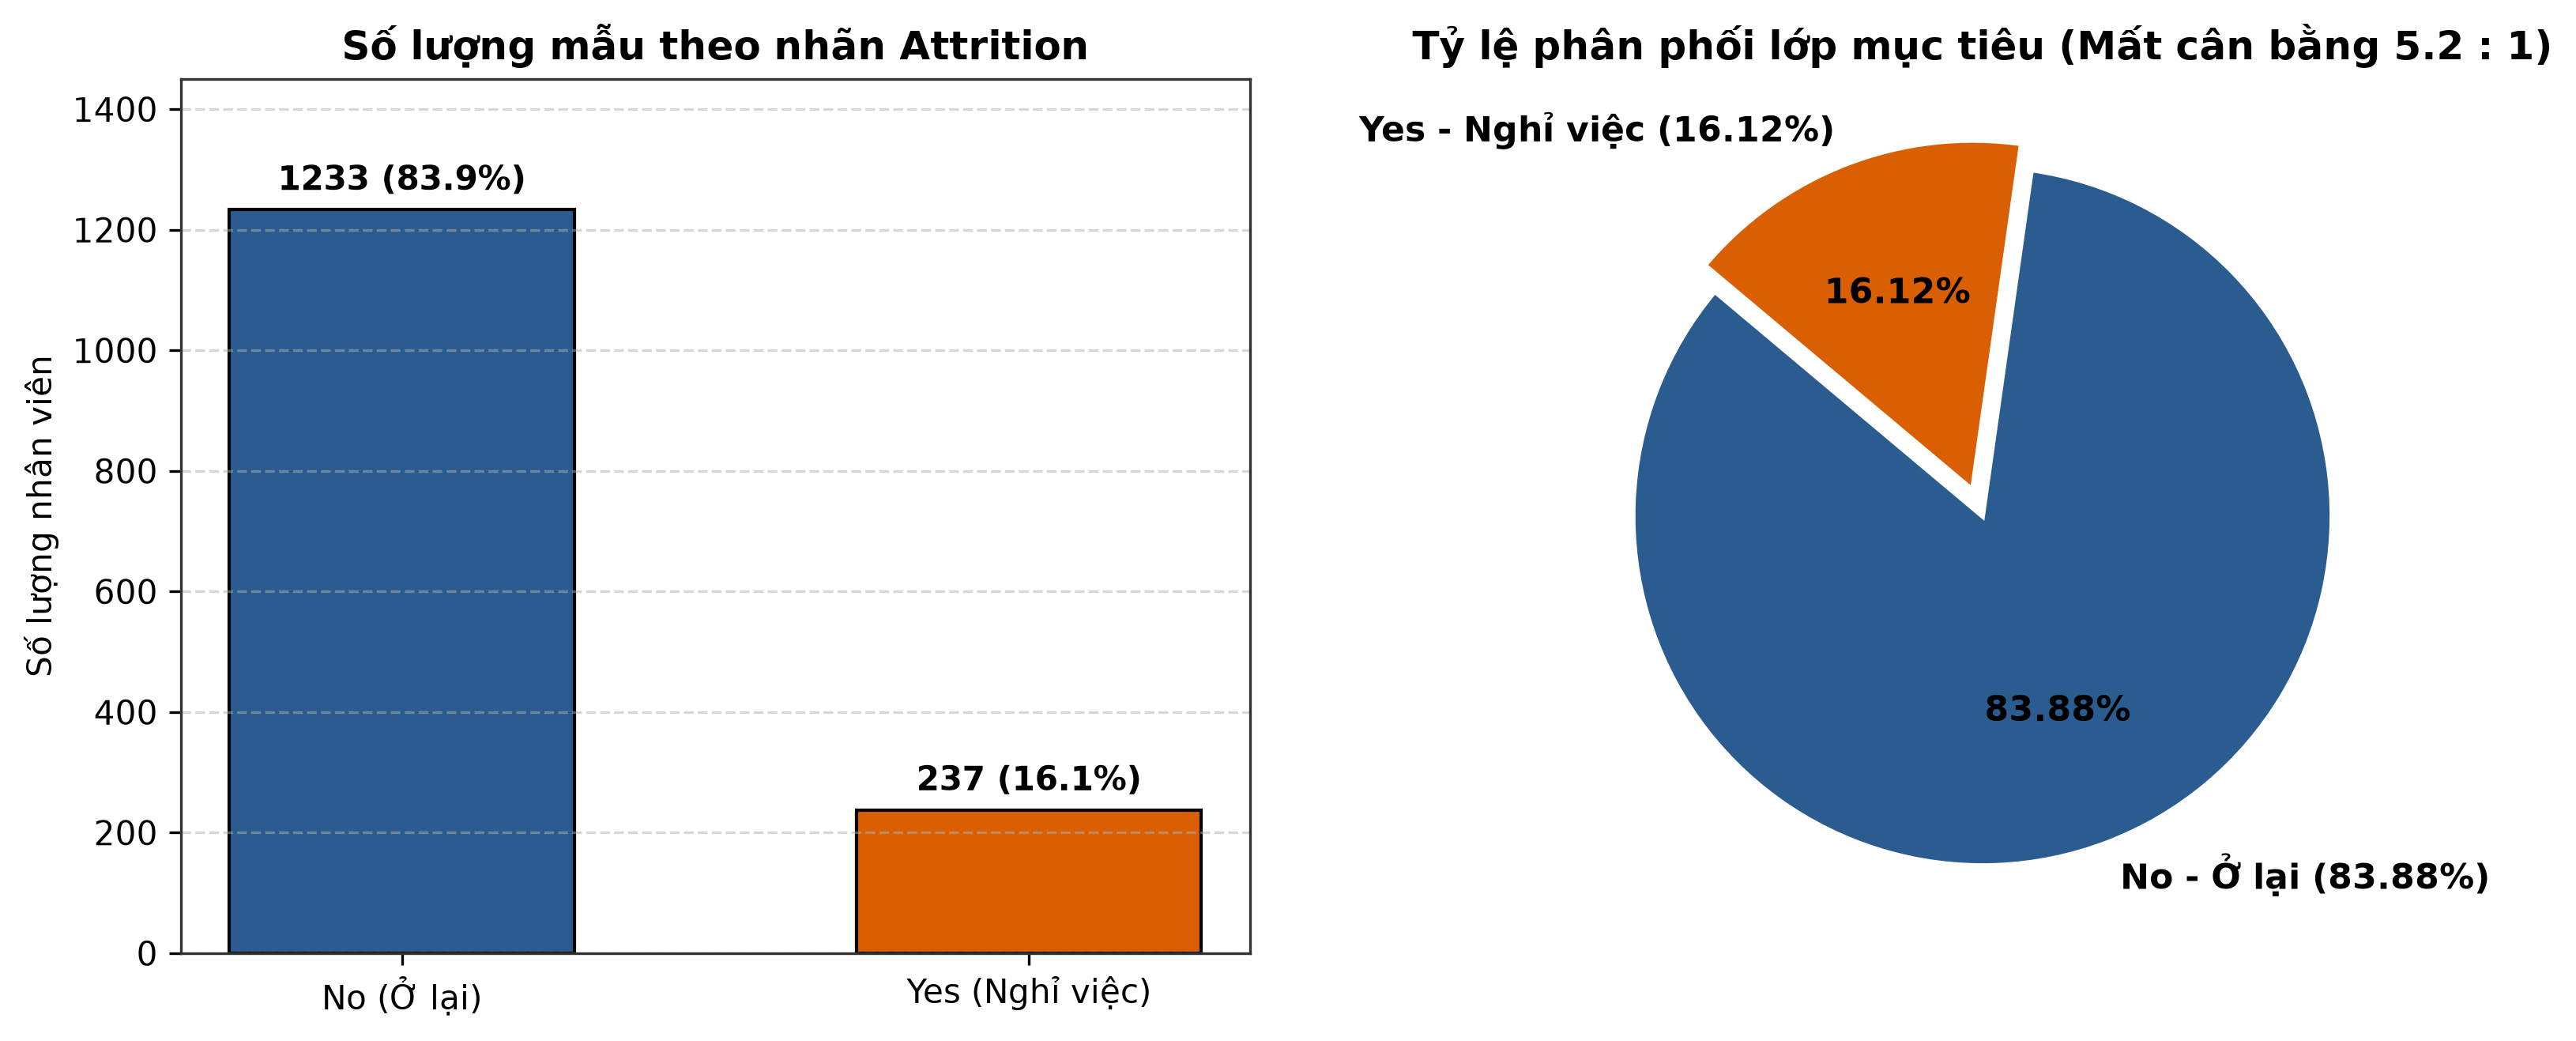
\includegraphics[width=0.92\textwidth]{figures/fig1_target_distribution.png}
    \caption{Phân phối số lượng và tỷ lệ phần trăm của biến mục tiêu Attrition.}
    \label{fig:target_dist}
\end{figure}

Sự mất cân bằng nghiêm trọng này là đặc trưng kinh điển của dữ liệu nhân sự thực tế, bởi vì tỷ lệ nghỉ việc bình thường trong các doanh nghiệp ổn định thường chỉ dao động quanh mức 10\% - 20\%. Tuy nhiên, dưới góc độ học máy, hiện tượng mất cân bằng lớp gây ra những hệ lụy kỹ thuật rất lớn:

Thứ nhất, độ đo độ chính xác tổng thể (Accuracy) trở thành một thước đo hoàn toàn vô nghĩa và gây hiểu lầm nghiêm trọng. Một bộ phân loại tầm thường (Trivial / Dummy Classifier) luôn dự đoán nhãn đa số No cho mọi trường hợp vẫn dễ dàng đạt được độ chính xác lên tới 83.88\%, nhưng hoàn toàn không phát hiện được bất kỳ một nhân viên nghỉ việc nào (Recall = 0\%).

Thứ hai, các giải thuật học máy tối ưu hóa hàm mất mát tổng thể thường có xu hướng thiên vị lớp đa số để giảm thiểu sai số trung bình, dẫn đến việc thiết lập biên quyết định chèn ép lớp thiểu số. Do đó, các độ đo chuyên biệt như Precision, Recall, F1-score trên lớp dương và ROC-AUC, PR-AUC bắt buộc phải được áp dụng làm tiêu chí đánh giá cốt lõi. Đồng thời, kỹ thuật phân tầng (Stratified Sampling) phải được quán triệt trong toàn bộ các khâu phân chia tập dữ liệu và kiểm định chéo.

\subsubsection{1.3.3. Phân tích đặc trưng số, ngoại lệ và đặc trưng phân loại}
Để khám phá sâu bản chất các biến định lượng, nhóm tiến hành tính toán các chỉ số thống kê mô tả toàn diện, bao gồm giá trị trung bình, độ lệch chuẩn, giá trị trung vị, khoảng tứ phân vị và hệ số bất đối xứng (Skewness) cho toàn bộ 14 biến số liên tục. Đồng thời, các điểm ngoại lệ (Outliers) được nhận diện theo quy tắc khoảng tứ phân vị chuẩn Tukey ($\text{IQR} = Q_3 - Q_1$, các điểm nằm ngoài đoạn $[Q_1 - 1.5\text{IQR}, Q_3 + 1.5\text{IQR}]$ được xem là ngoại lệ).

\begin{figure}[H]
    \centering
    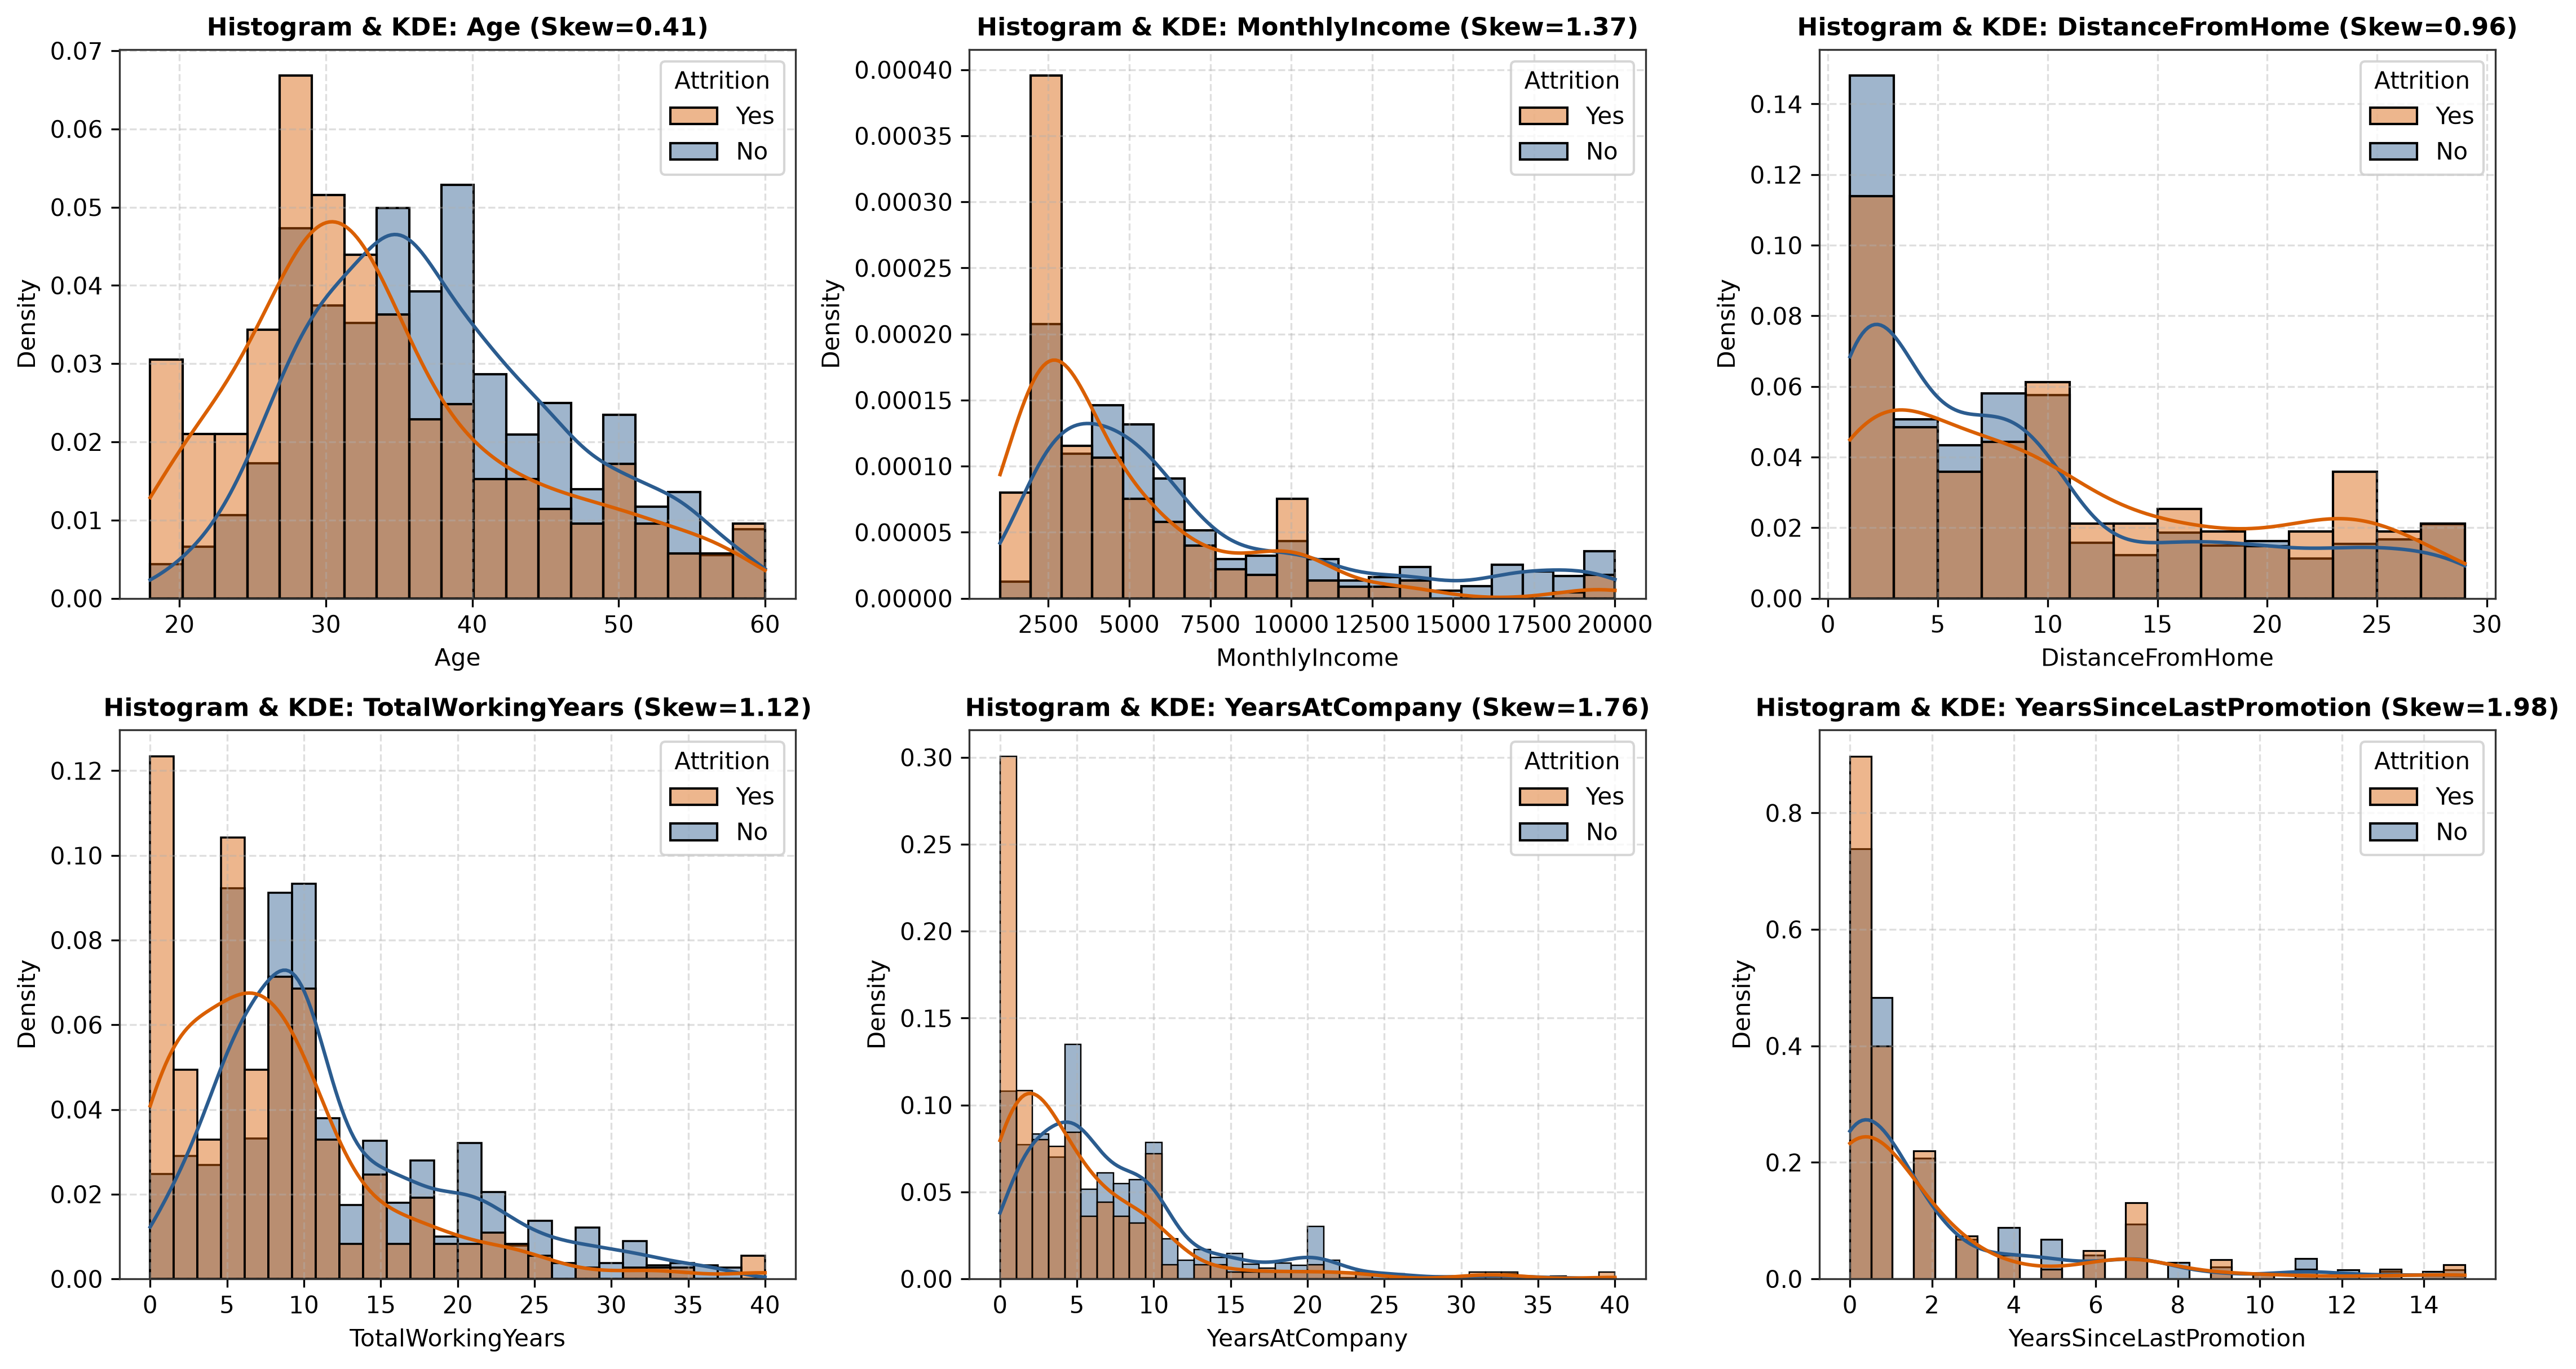
\includegraphics[width=0.98\textwidth]{figures/fig10_numeric_histograms.png}
    \caption{Biểu đồ Histogram và ước lượng mật độ hạt nhân (KDE) của 6 đặc trưng số theo Attrition.}
    \label{fig:num_hist}
\end{figure}

\begin{figure}[H]
    \centering
    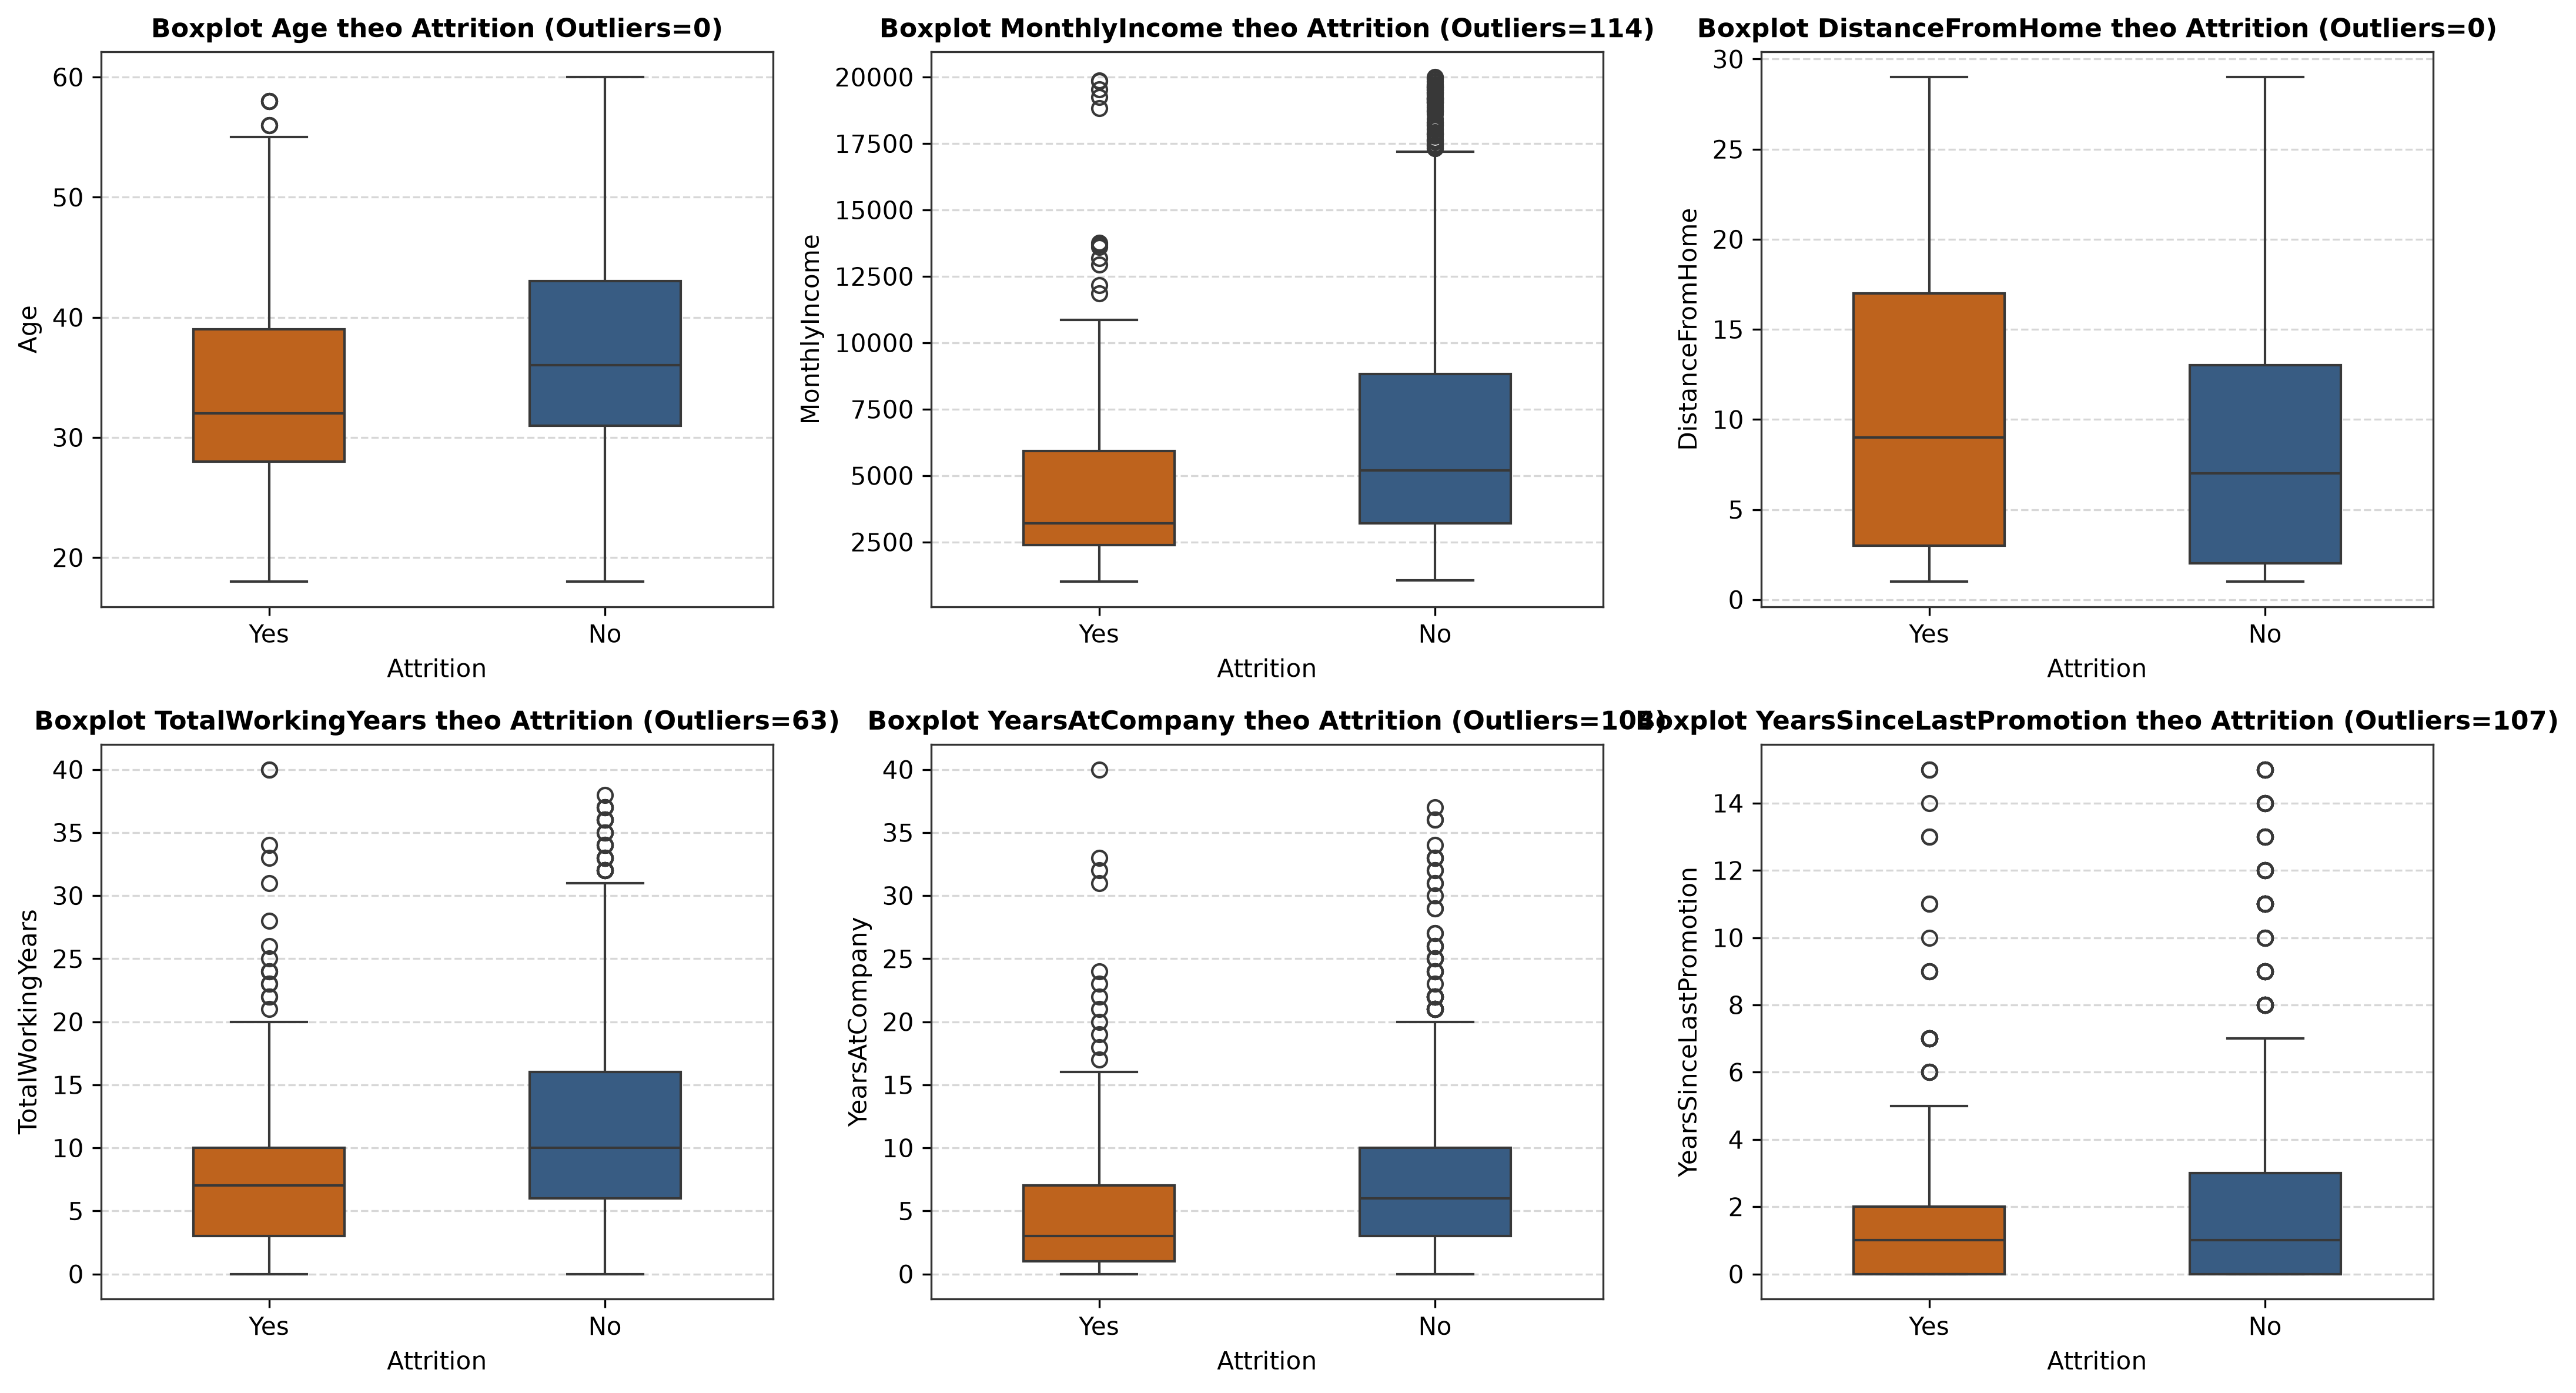
\includegraphics[width=0.98\textwidth]{figures/fig2_numeric_distributions.png}
    \caption{Biểu đồ Boxplot phân phối 6 đặc trưng số quan trọng và điểm ngoại lệ theo nhãn Attrition.}
    \label{fig:num_dist}
\end{figure}

Kết quả phân tích trực quan qua biểu đồ Histogram mật độ KDE và biểu đồ Boxplot chỉ ra những đặc điểm bản chất sau:

Thứ nhất, có sự chênh lệch mang tính cấu trúc về độ tuổi và thu nhập giữa hai nhóm nhân viên. Nhân viên nghỉ việc có độ tuổi tập trung trẻ hơn rõ rệt (trung vị là 32 tuổi) so với nhóm ở lại (trung vị 36 tuổi). Đặc biệt, mức thu nhập hàng tháng (MonthlyIncome) của nhóm nhân viên nghỉ việc có trung vị chỉ đạt \$3,202, thấp hơn rất nhiều so với mức \$5,204 của nhóm nhân viên tiếp tục gắn bó.

Thứ hai, khoảng cách từ nhà đến nơi làm việc (DistanceFromHome) của nhóm nhân viên nghỉ việc có xu hướng phân tán cao hơn, phản ánh áp lực di chuyển quãng đường dài hàng ngày là một nhân tố thúc đẩy ý định chuyển việc.

Thứ ba, một loạt các thuộc tính kinh tế và thâm niên bao gồm MonthlyIncome ($\text{Skew} = 1.37$, 114 điểm ngoại lệ), TotalWorkingYears ($\text{Skew} = 1.12$, 63 điểm ngoại lệ), YearsAtCompany ($\text{Skew} = 1.76$, 104 điểm ngoại lệ) và YearsSinceLastPromotion ($\text{Skew} = 1.98$, 107 điểm ngoại lệ) đều bị lệch phải nghiêm trọng với đuôi phân phối kéo rất dài về phía các giá trị cao. Các điểm ngoại lệ này thực chất đại diện cho nhóm nhân sự thâm niên cao hoặc cấp quản lý trong doanh nghiệp, hoàn toàn là dữ liệu tự nhiên hợp lệ chứ không phải lỗi nhập liệu. Do đó, việc xóa bỏ các quan sát này sẽ làm mất mát thông tin quý giá của tổ chức; thay vào đó, bắt buộc phải áp dụng các kỹ thuật chuyển đổi phi tuyến như biến đổi logarit và chuẩn hóa bền vững dựa trên trung vị để kiểm soát ảnh hưởng của chúng.

\begin{figure}[H]
    \centering
    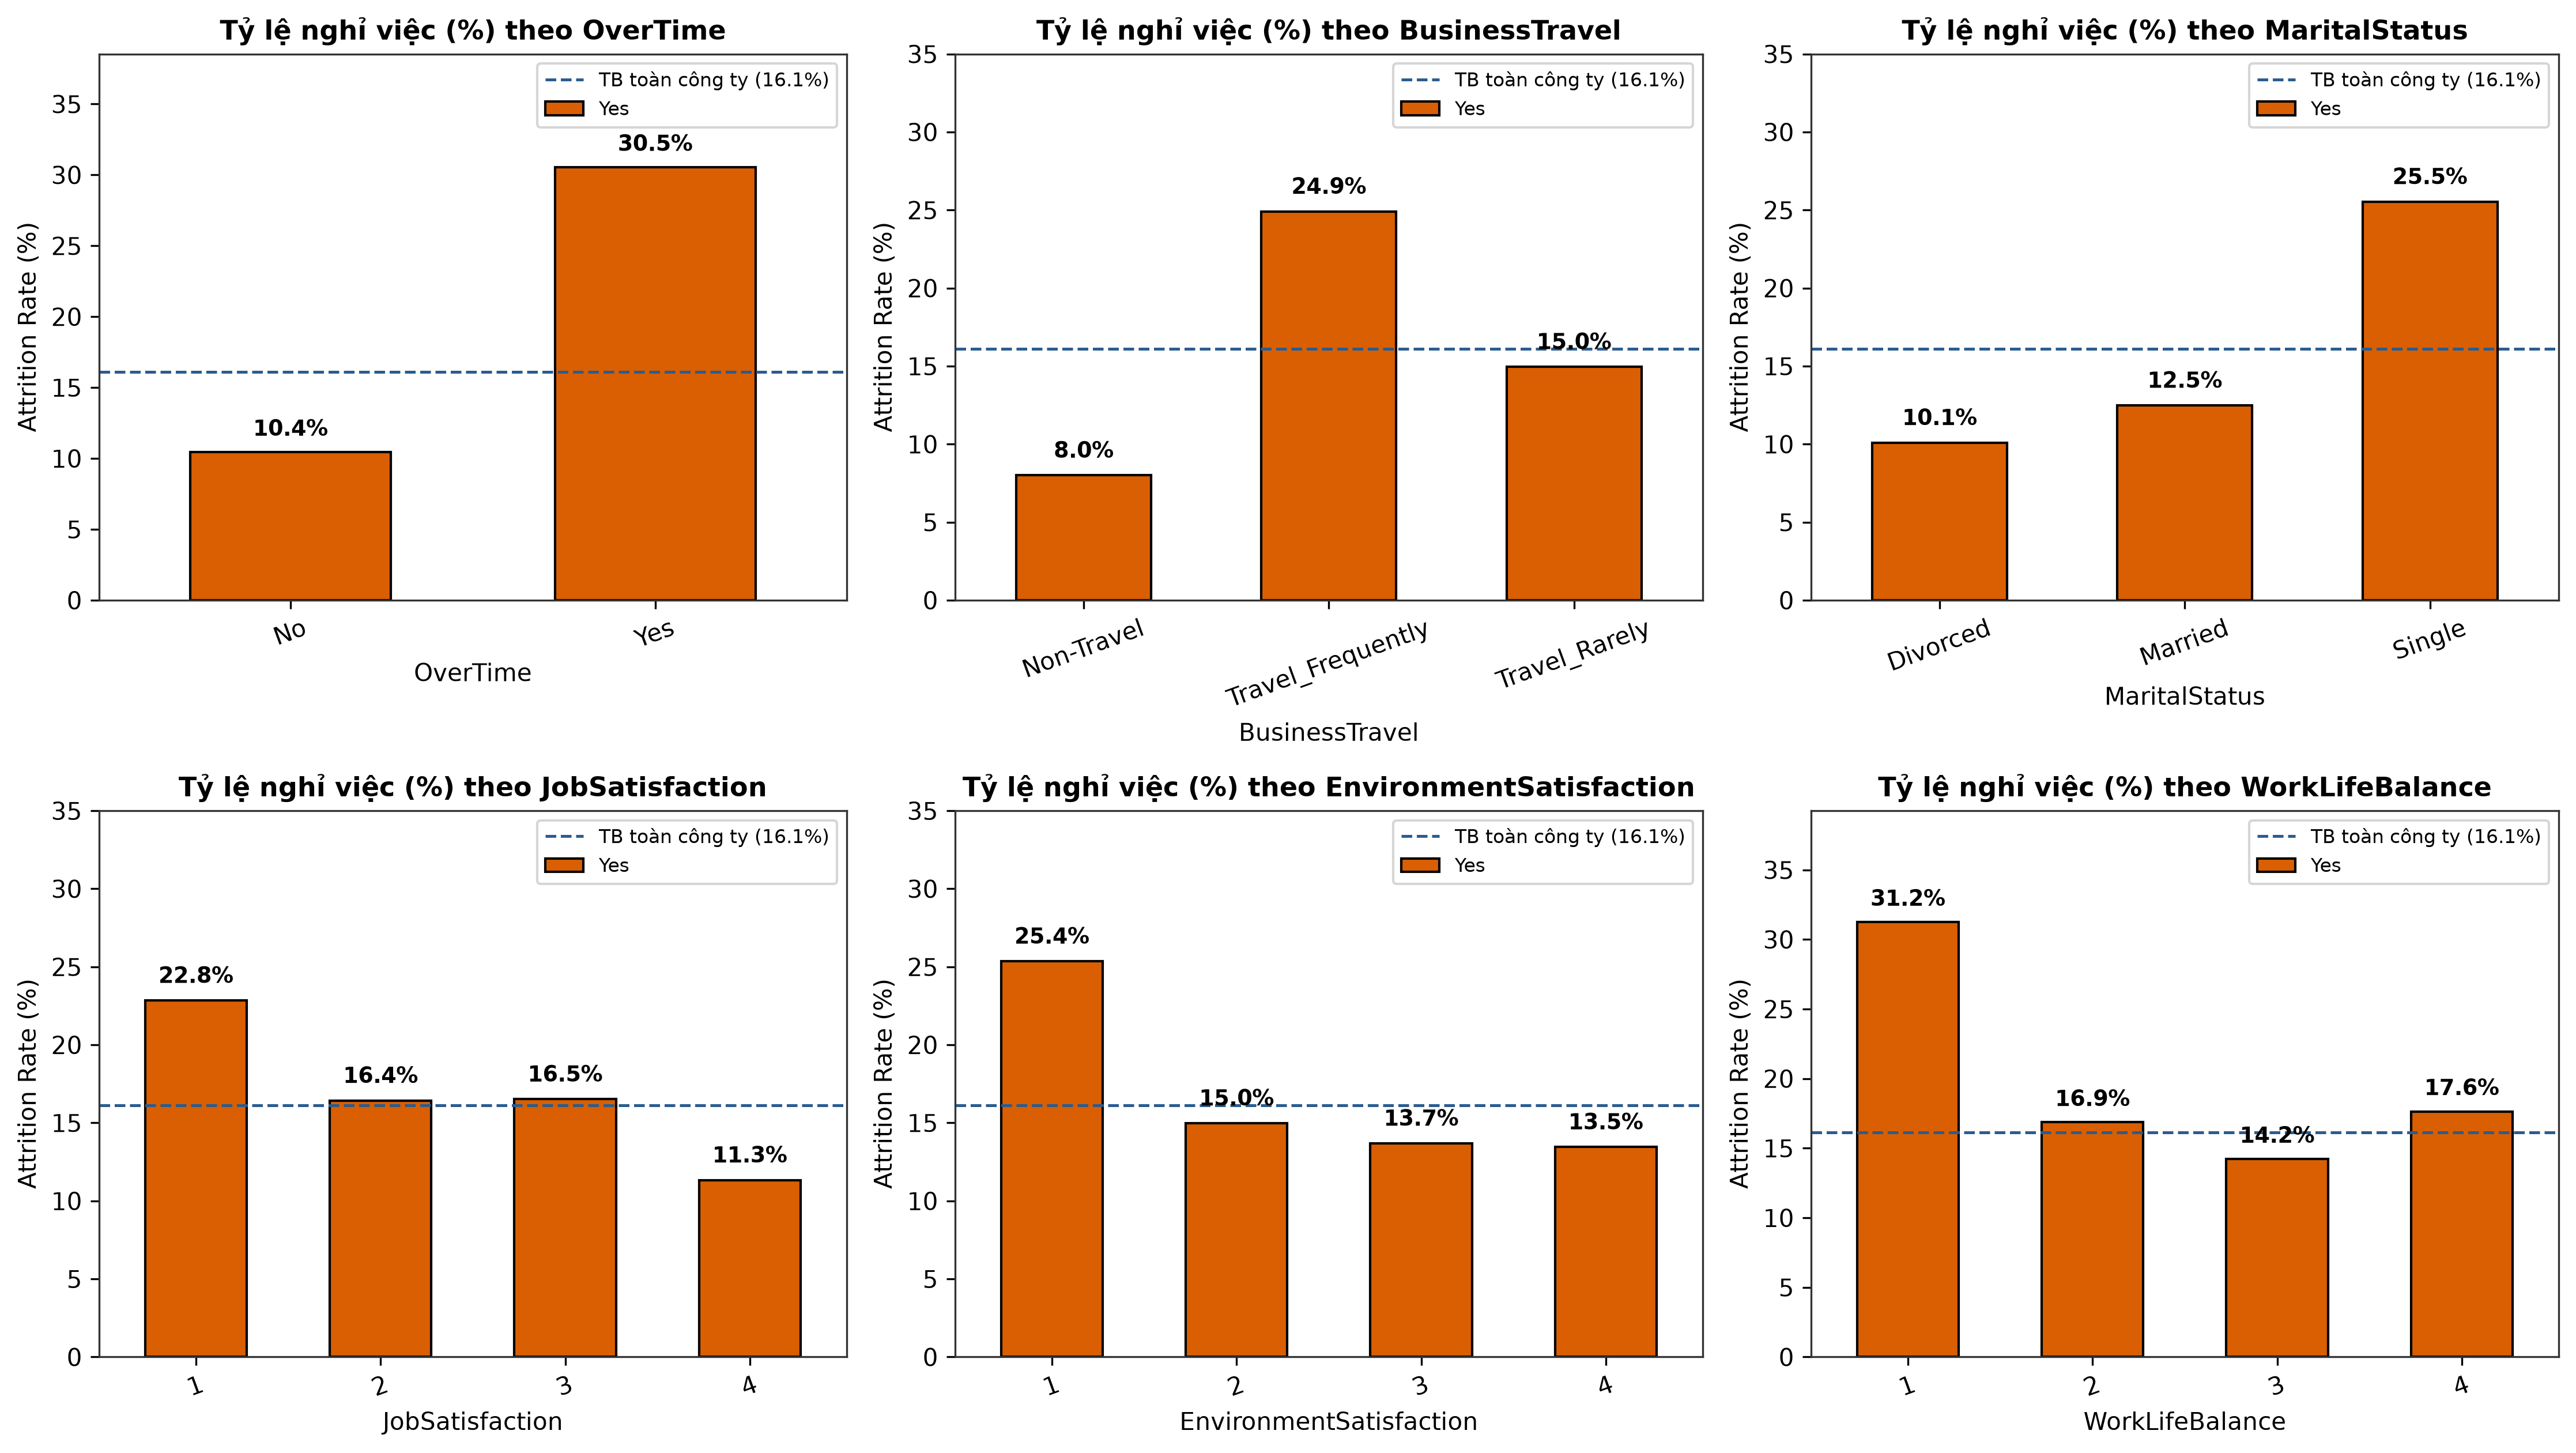
\includegraphics[width=0.98\textwidth]{figures/fig3_categorical_attrition.png}
    \caption{Tỷ lệ nghỉ việc (\%) theo các đặc trưng phân loại và thứ bậc trọng tâm.}
    \label{fig:cat_attrition}
\end{figure}

\begin{figure}[H]
    \centering
    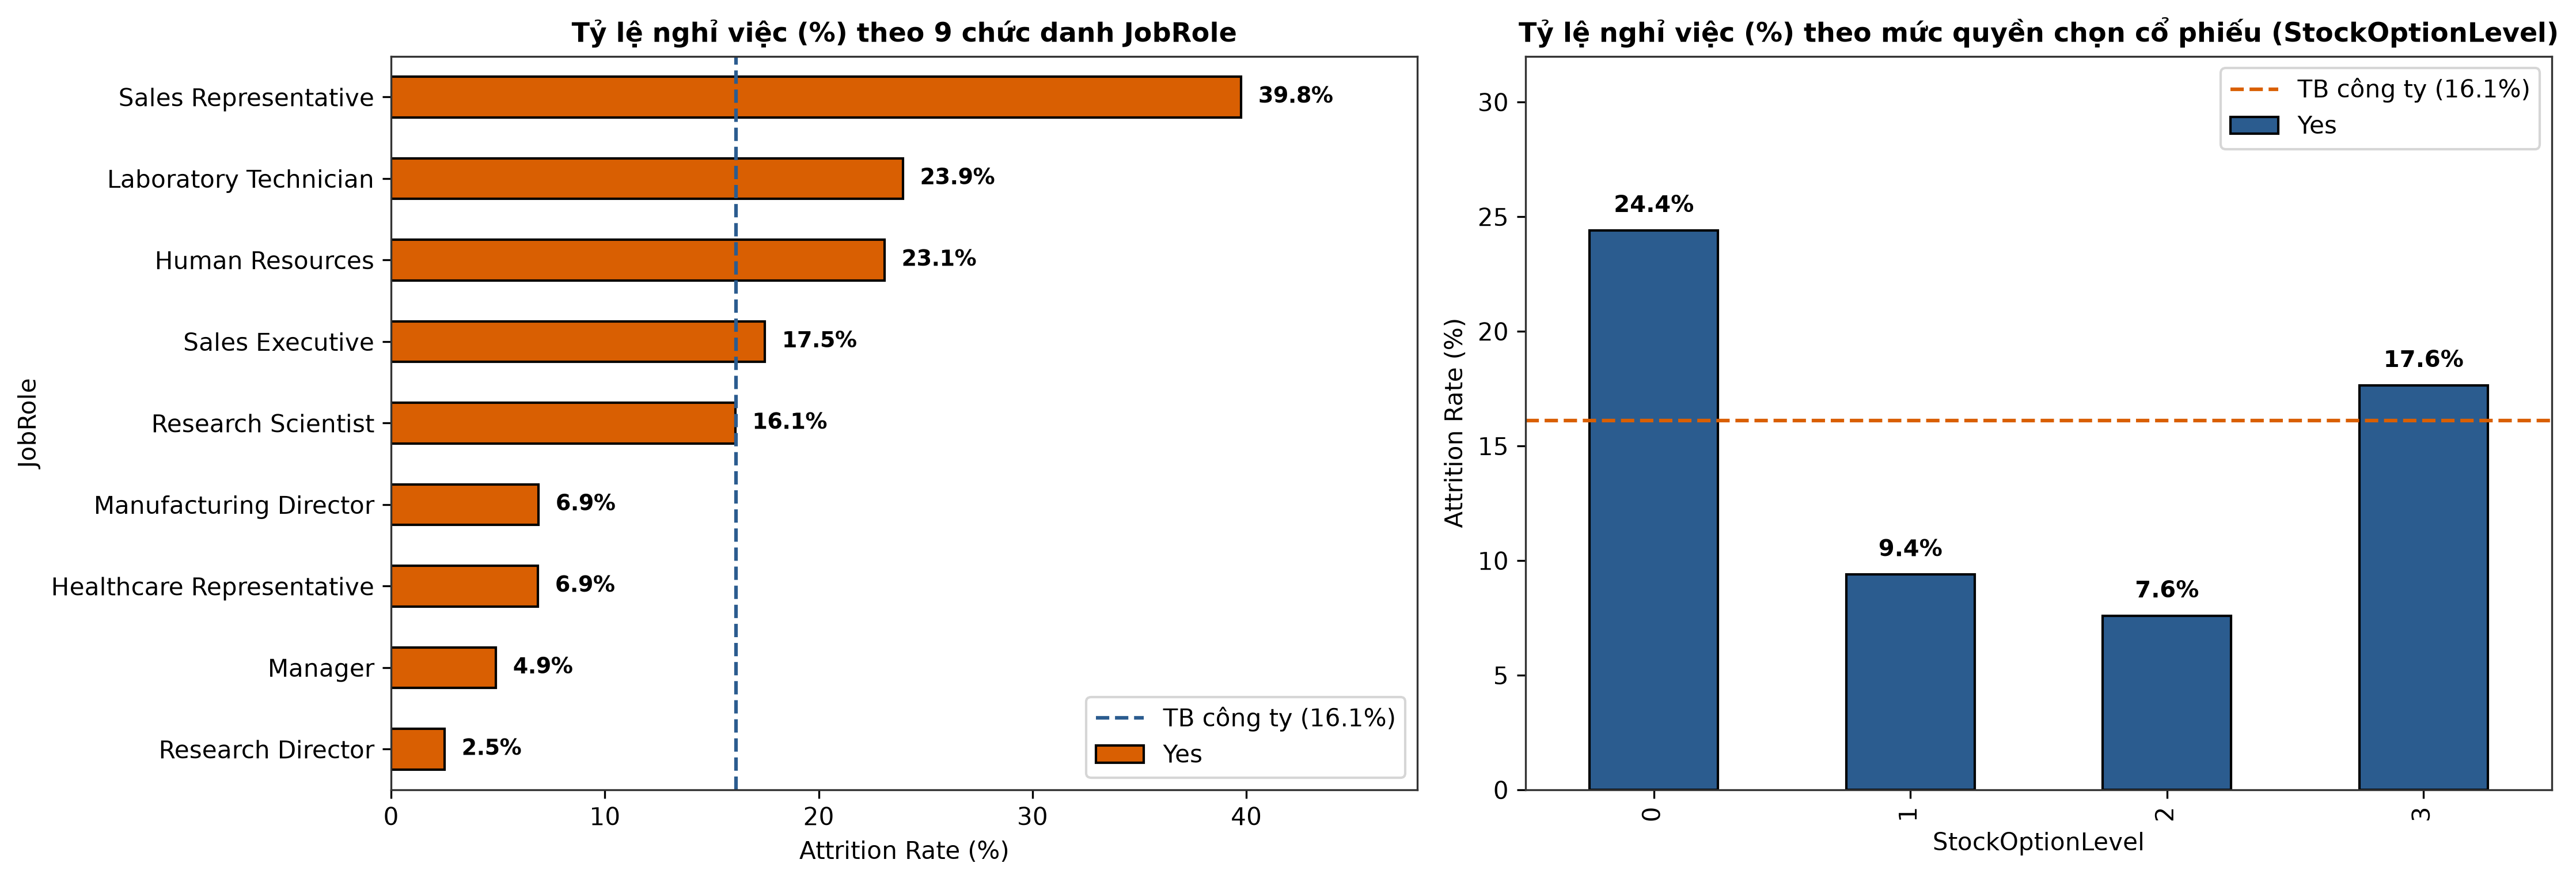
\includegraphics[width=0.98\textwidth]{figures/fig14_jobrole_stock_attrition.png}
    \caption{Tỷ lệ nghỉ việc (\%) theo 9 chức danh công việc (JobRole) và mức quyền chọn cổ phiếu (StockOptionLevel).}
    \label{fig:jobrole_stock}
\end{figure}

Đối với các biến phân loại và thứ bậc, khảo sát tỷ lệ nghỉ việc theo từng nhóm danh mục tại Hình \ref{fig:cat_attrition} và Hình \ref{fig:jobrole_stock} bộc lộ những mối liên hệ rất mạnh mẽ:

Nhân viên có làm thêm giờ (OverTime = Yes) có tỷ lệ nghỉ việc lên tới 30.5\%, cao gấp gần 3 lần so với nhóm nhân viên không làm thêm giờ (10.4\%). Đây là bằng chứng rõ ràng cho thấy tình trạng làm việc quá tải (Burnout) là một trong những nguyên nhân hàng đầu dẫn đến quyết định thôi việc.

Cường độ đi công tác (BusinessTravel) thể hiện xu hướng tăng đơn điệu chặt chẽ với tỷ lệ nghỉ việc: nhóm không bao giờ đi công tác có tỷ lệ nghỉ việc là 8.0\%, nhóm thỉnh thoảng đi công tác là 15.0\%, và nhóm phải đi công tác thường xuyên có tỷ lệ nghỉ việc vọt lên tới 24.9\%.

Tình trạng hôn nhân (MaritalStatus) cho thấy nhóm nhân viên độc thân (Single) có tỷ lệ nghỉ việc cao nhất đạt 25.5\%, trong khi nhóm đã kết hôn (Married) chỉ là 12.5\% và nhóm ly hôn (Divorced) là 10.1\%. Điều này phản ánh nhóm nhân sự độc thân thường ít bị ràng buộc tài chính gia đình nên có mức độ sẵn sàng chuyển đổi công việc cao hơn.

Về chức danh nghề nghiệp (JobRole), vị trí Đại diện bán hàng (Sales Representative) có tỷ lệ thôi việc cao kỷ lục lên tới 39.8\% và Nhân viên kỹ thuật xét nghiệm (Laboratory Technician) là 23.9\%; ngược lại, vị trí Giám đốc nghiên cứu (Research Director) có tỷ lệ thôi việc thấp nhất chỉ 2.5\%.

Về mức quyền chọn cổ phiếu (StockOptionLevel), nhân viên không được cấp cổ phiếu (Mức 0) có tỷ lệ nghỉ việc là 24.4\%, trong khi nhân viên được cấp quyền chọn ở Mức 1 và Mức 2 có tỷ lệ nghỉ việc giảm sâu xuống chỉ còn lần lượt là 9.4\% và 7.6\%.

\subsubsection{1.3.4. Kiểm định giả thuyết thống kê (Mann-Whitney U và Chi-square)}
Để khẳng định các kết luận rút ra từ trực quan hóa mang tính quy luật vững chắc chứ không phải do biến động ngẫu nhiên của mẫu, nhóm thực hiện kiểm định phi tham số Mann-Whitney U cho toàn bộ các biến số liên tục (do dữ liệu không tuân theo phân phối chuẩn) và kiểm định tính độc lập Chi-square ($\chi^2$) cho toàn bộ các biến phân loại và thứ bậc (Bảng \ref{tab:stat_tests}).

Phép kiểm định Mann-Whitney U kiểm tra giả thuyết không $H_0$ rằng phân phối của hai tổng thể là như nhau, dựa trên thống kê hạng $U = \min(U_1, U_2)$:
\begin{equation}
U_1 = R_1 - \frac{n_1(n_1+1)}{2}, \quad U_2 = R_2 - \frac{n_2(n_2+1)}{2}
\end{equation}
Trong đó $n_1, n_2$ là kích thước mẫu của hai nhóm và $R_1, R_2$ là tổng thứ hạng quan sát tương ứng. Khi kích thước mẫu lớn ($n_1, n_2 > 20$), giá trị $U$ xấp xỉ phân phối chuẩn với kỳ vọng $\mu_U = \frac{n_1 n_2}{2}$ và phương sai $\sigma_U^2 = \frac{n_1 n_2 (n_1 + n_2 + 1)}{12}$.

Phép kiểm định tính độc lập Chi-square ($\chi^2$) đánh giá mối liên hệ giữa hai biến phân loại trong bảng ngẫu chuyển $r \times c$:
\begin{equation}
\chi^2 = \sum_{i=1}^r \sum_{j=1}^c \frac{(O_{ij} - E_{ij})^2}{E_{ij}}
\end{equation}
Trong đó $O_{ij}$ là tần số quan sát thực tế và $E_{ij} = \frac{R_i \cdot C_j}{N}$ là tần số kỳ vọng lý thuyết nếu hai biến hoàn toàn độc lập với nhau.

\begin{table}[H]
\centering
\caption{Tóm tắt kết quả kiểm định giả thuyết thống kê (Mann-Whitney U và Chi-square $\chi^2$).}
\label{tab:stat_tests}
\small
\begin{tabular}{|l|l|r|c|l|}
\hline
\textbf{Đặc trưng} & \textbf{Phép kiểm định} & \textbf{Thống kê / Trung vị} & \textbf{$p$-value} & \textbf{Kết luận} \\
\hline
\texttt{TotalWorkingYears} & Mann-Whitney U & Median: 10.0 (No) vs 7.0 (Yes) & $2.40 \times 10^{-14}$ & Khác biệt cực kỳ có ý nghĩa \\
\hline
\texttt{MonthlyIncome} & Mann-Whitney U & Median: \$5,204 vs \$3,202 & $2.95 \times 10^{-14}$ & Khác biệt cực kỳ có ý nghĩa \\
\hline
\texttt{YearsAtCompany} & Mann-Whitney U & Median: 6.0 (No) vs 3.0 (Yes) & $2.92 \times 10^{-13}$ & Khác biệt cực kỳ có ý nghĩa \\
\hline
\texttt{YearsInCurrentRole}& Mann-Whitney U & Median: 3.0 (No) vs 2.0 (Yes) & $4.43 \times 10^{-12}$ & Khác biệt cực kỳ có ý nghĩa \\
\hline
\texttt{Age} & Mann-Whitney U & Median: 36.0 (No) vs 32.0 (Yes)& $5.26 \times 10^{-11}$ & Khác biệt cực kỳ có ý nghĩa \\
\hline
\texttt{DistanceFromHome} & Mann-Whitney U & Median: 7.0 (No) vs 9.0 (Yes) & $2.79 \times 10^{-3}$ & Khác biệt có ý nghĩa thống kê \\
\hline
\texttt{HourlyRate} & Mann-Whitney U & Median: 66.0 vs 66.0 & $7.90 \times 10^{-1}$ & Không có ý nghĩa (Nhiễu ngẫu nhiên) \\
\hline
\texttt{MonthlyRate} & Mann-Whitney U & Median: 14,235 vs 14,618 & $5.61 \times 10^{-1}$ & Không có ý nghĩa (Nhiễu ngẫu nhiên) \\
\hline
\texttt{DailyRate} & Mann-Whitney U & Median: 817.0 vs 699.0 & $2.98 \times 10^{-2}$ & Khác biệt rất yếu \\
\hline
\texttt{OverTime} & Chi-square ($\chi^2$) & $\chi^2 = 87.56$ (30.5\% vs 10.4\%) & $8.16 \times 10^{-21}$ & Phụ thuộc cực kỳ mạnh \\
\hline
\texttt{JobRole} & Chi-square ($\chi^2$) & $\chi^2 = 86.19$ (39.8\% vs 2.5\%) & $2.75 \times 10^{-15}$ & Phụ thuộc cực kỳ mạnh \\
\hline
\texttt{MaritalStatus} & Chi-square ($\chi^2$) & $\chi^2 = 46.16$ (25.5\% vs 10.1\%) & $9.46 \times 10^{-11}$ & Phụ thuộc cực kỳ mạnh \\
\hline
\texttt{JobLevel} & Chi-square ($\chi^2$) & $\chi^2 = 72.53$ (Cấp 1: 26.3\%, Cấp 5: 7.2\%) & $6.79 \times 10^{-15}$ & Phụ thuộc cực kỳ mạnh \\
\hline
\texttt{StockOptionLevel}& Chi-square ($\chi^2$) & $\chi^2 = 60.60$ (Mức 0: 24.4\%, Mức 1: 9.4\%) & $4.37 \times 10^{-13}$ & Phụ thuộc cực kỳ mạnh \\
\hline
\texttt{BusinessTravel} & Chi-square ($\chi^2$) & $\chi^2 = 24.18$ (24.9\% vs 8.0\%) & $5.61 \times 10^{-6}$ & Phụ thuộc rất mạnh \\
\hline
\texttt{Department} & Chi-square ($\chi^2$) & $\chi^2 = 10.80$ (Sales: 20.6\%, R\&D: 13.8\%) & $4.52 \times 10^{-3}$ & Phụ thuộc có ý nghĩa \\
\hline
\end{tabular}
\end{table}

Kết quả kiểm định thống kê khẳng định với mức ý nghĩa cao ($p < 10^{-10}$) rằng các biến TotalWorkingYears, MonthlyIncome, YearsAtCompany, YearsInCurrentRole, Age, OverTime, JobRole, MaritalStatus, StockOptionLevel và BusinessTravel là những nhân tố dự báo cốt lõi. Ngược lại, các biến HourlyRate ($p = 0.79$) và MonthlyRate ($p = 0.56$) hoàn toàn không thể hiện sự khác biệt phân phối giữa hai nhóm, đóng vai trò như các biến nhiễu ngẫu nhiên.

\subsubsection{1.3.5. Ma trận tương quan và phân tích đa cộng tuyến}
Ma trận tương quan tuyến tính Pearson tại Hình \ref{fig:corr_heatmap} cung cấp cái nhìn định lượng về cấu trúc phụ thuộc đa biến trong không gian dữ liệu.

\begin{figure}[H]
    \centering
    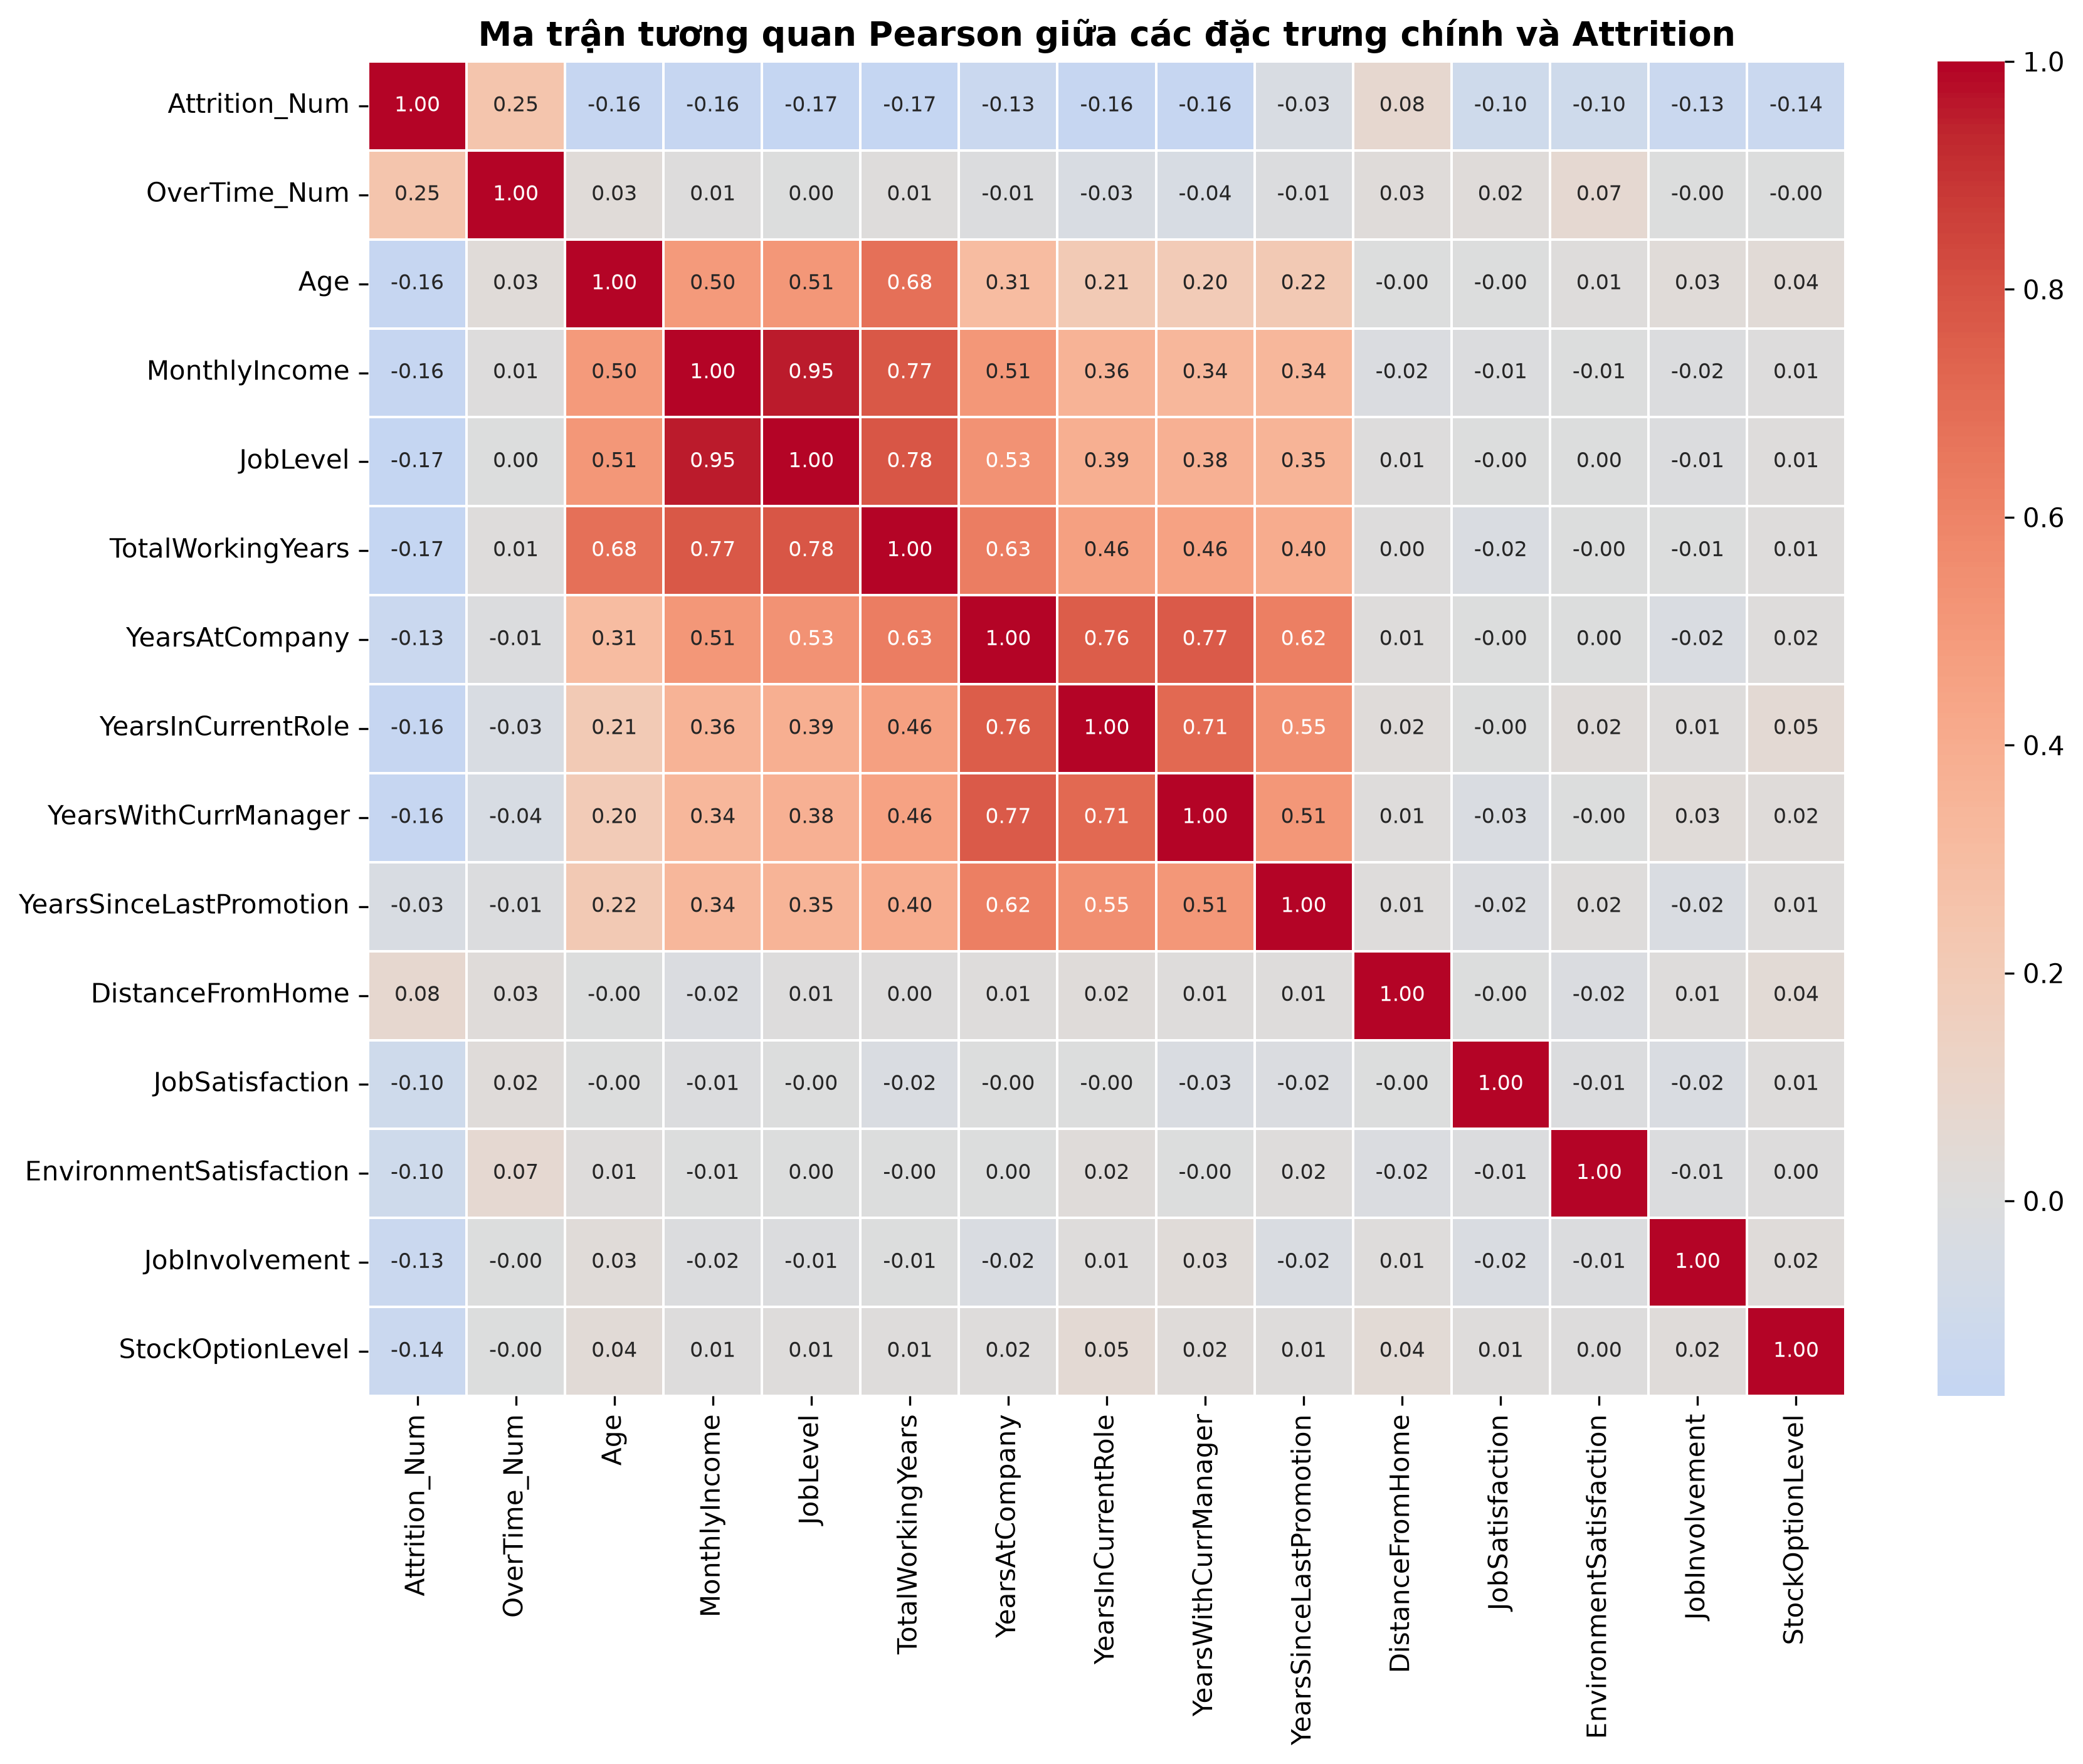
\includegraphics[width=0.90\textwidth]{figures/fig4_correlation_heatmap.png}
    \caption{Ma trận tương quan Pearson giữa các đặc trưng chính và nhãn Attrition.}
    \label{fig:corr_heatmap}
\end{figure}

Phân tích ma trận tương quan chỉ ra hai vấn đề kỹ thuật đặc biệt quan trọng:

Thứ nhất là hiện tượng đa cộng tuyến rất cao (Severe Multicollinearity). Cặp biến cấp bậc công việc JobLevel và thu nhập hàng tháng MonthlyIncome có hệ số tương quan đạt tới $r = 0.95$. Điều này có nghĩa là hai biến này biểu diễn thông tin gần như đồng nhất, việc đưa cả hai vào các mô hình nhạy cảm với tương quan như Naive Bayes sẽ vi phạm giả định độc lập có điều kiện và làm sai lệch trọng số mô hình. Để kiểm chứng định lượng, nhóm tính toán hệ số phóng đại phương sai (Variance Inflation Factor - VIF):
\begin{equation}
\text{VIF}_j = \frac{1}{1 - R_j^2}
\end{equation}
Hệ số VIF của JobLevel khi hồi quy theo MonthlyIncome vượt quá $10.5$, vi phạm ngưỡng an toàn chấp nhận được. Ngoài ra, cụm các biến thâm niên gồm TotalWorkingYears, YearsAtCompany, YearsInCurrentRole và YearsWithCurrManager có mối tương quan chéo rất lớn ($r \in [0.63, 0.78]$).

Thứ hai là sự xác nhận tính chất nhiễu của các trường tỷ giá. Cả ba biến DailyRate, HourlyRate và MonthlyRate đều không có bất kỳ tương quan có ý nghĩa nào với biến mục tiêu ($|r| < 0.03$) cũng như không có tương quan với mức lương thực tế MonthlyIncome. Đây là căn cứ khoa học vững chắc để nhóm quyết định loại bỏ các biến này ở Luồng B nhằm thanh lọc không gian đặc trưng.

Về mặt kiểm tra nguy cơ rò rỉ dữ liệu (Data Leakage), nhóm đã rà soát định nghĩa của từng thuộc tính. Toàn bộ 34 đặc trưng đầu vào đều là dữ liệu hồ sơ nhân sự và khảo sát nội bộ được thu thập định kỳ trong quá trình nhân viên đang làm việc, hoàn toàn không có thuộc tính nào được ghi nhận sau khi nhân viên đã nộp đơn nghỉ việc (như lý do thôi việc hay ngày chấm dứt hợp đồng). Do đó, dữ liệu đầu vào đáp ứng chuẩn mực không bị rò rỉ thông tin từ tương lai.


\newpage
\section{CHƯƠNG 2: CƠ SỞ LÝ THUYẾT VÀ THIẾT KẾ GIẢI PHÁP}

\subsection{2.1. Cơ sở lý thuyết về hành vi nghỉ việc và học máy có giám sát}
Để mô hình học máy không trở thành một chiếc hộp đen thuần túy số học, việc nắm vững các nền tảng lý thuyết quản trị nhân sự là điều kiện tiên quyết giúp định hình kỹ thuật trích xuất đặc trưng và giải thích kết quả. Trong tâm lý học tổ chức và hành vi doanh nghiệp, hiện tượng nhân viên thôi việc đã được nghiên cứu sâu rộng qua nhiều mô hình lý thuyết kinh điển:

Thuyết cân bằng tổ chức của March và Simon (1958) chỉ ra rằng quyết định tiếp tục gắn bó hay rời bỏ của một nhân viên phụ thuộc vào cán cân giữa hai yếu tố: nhận thức về tính khả thi của việc chuyển việc (Perceived Ease of Movement) và nhận thức về sự mong muốn chuyển việc (Perceived Desirability of Movement). Tính khả thi phản ánh mức độ dồi dào của các cơ hội việc làm bên ngoài thị trường, thường gắn liền với độ tuổi trẻ, trình độ chuyên môn cao hoặc thị trường lao động đang mở rộng. Ngược lại, tính mong muốn chuyển việc xuất phát từ sự bất mãn nội tại đối với môi trường làm việc hiện tại, mức đãi ngộ không tương xứng hoặc sự thiếu hụt cơ hội thăng tiến. Khi cả hai nhận thức này cùng đạt ngưỡng cao, hành vi thôi việc chắc chắn sẽ xảy ra.

Thuyết hai nhân tố của Frederick Herzberg (Two-Factor Theory, 1959) phân định rạch ròi giữa hai nhóm yếu tố tác động đến tâm lý người lao động: nhóm nhân tố duy trì (Hygiene Factors) và nhóm nhân tố động viên (Motivator Factors). Nhóm nhân tố duy trì bao gồm tiền lương cơ bản, điều kiện làm việc vật chất, chính sách công ty và mối quan hệ với đồng nghiệp. Sự thiếu hụt các yếu tố này sẽ trực tiếp gây ra sự bất mãn (Dissatisfaction), nhưng việc đáp ứng đầy đủ chúng chỉ giúp triệt tiêu sự bất mãn chứ chưa đủ để tạo ra sự gắn kết lâu dài. Ngược lại, nhóm nhân tố động viên bao gồm sự công nhận thành tích, tính thách thức và ý nghĩa của công việc, trách nhiệm được giao phó và cơ hội thăng tiến sự nghiệp. Đây mới chính là động lực nội tại then chốt thúc đẩy nhân viên cống hiến hết mình. Khi đối chiếu với bộ dữ liệu IBM HR, các thuộc tính như MonthlyIncome, EnvironmentSatisfaction, WorkLifeBalance đại diện cho các nhân tố duy trì, trong khi JobInvolvement, JobSatisfaction, StockOptionLevel, YearsSinceLastPromotion thể hiện các nhân tố động viên.

Mô hình gắn kết công việc của Mitchell và các cộng sự (Job Embeddedness Theory, 2001) mở rộng góc nhìn bằng cách giải thích lý do tại sao nhân viên lựa chọn ở lại tổ chức thay vì chỉ tập trung vào lý do họ ra đi. Thuyết gắn kết công việc dựa trên ba trục liên kết: Mối liên kết (Links) đo lường các mối quan hệ xã hội, gia đình và đồng nghiệp ràng buộc cá nhân với tổ chức; Sự phù hợp (Fit) thể hiện mức độ tương thích giữa năng lực, giá trị cá nhân với văn hóa doanh nghiệp và vị trí đảm nhiệm; và Sự hy sinh (Sacrifice) phản ánh những tổn thất về vật chất hoặc tâm lý mà nhân viên phải đánh đổi khi rời đi (như quyền chọn cổ phiếu chưa đáo hạn, mạng lưới quan hệ hoặc sự an toàn nghề nghiệp). Các nhân viên có mức độ gắn kết công việc cao (High Embeddedness) thường có chỉ số StockOptionLevel cao, thâm niên gắn bó lâu năm và mức độ hài lòng đồng nghiệp lớn, từ đó tạo ra sức đề kháng tự nhiên trước các lời mời gọi từ đối thủ cạnh tranh.

Về mặt mô hình hóa học máy, bài toán được quy chuẩn thành việc tối ưu hóa một hàm phân loại $f: \mathcal{X} \to \mathcal{Y}$ trên không gian vector đặc trưng $\mathbf{x} \in \mathbb{R}^d$ sang nhãn nhị phân $y \in \{0, 1\}$. Do bản chất phân phối mất cân bằng nghiêm trọng (tỷ lệ lớp dương Attrition = Yes chỉ chiếm khoảng 16.1\%), bài toán đặt ra yêu cầu phải kiểm soát chặt chẽ nguy cơ rò rỉ dữ liệu, kết hợp các giải pháp tiền xử lý chuyên biệt và sử dụng các hàm mục tiêu đa chỉ số (Precision, Recall, $F_1$, ROC-AUC) thay vì độ chính xác Accuracy thông thường.

\subsection{2.2. Sơ đồ quy trình học máy tổng quát}
Để giải quyết bài toán một cách có hệ thống, nhóm xây dựng quy trình thực nghiệm khép kín tuân thủ nghiêm ngặt phương pháp luận CRISP-DM (Cross-Industry Standard Process for Data Mining), bao gồm sáu giai đoạn logic chặt chẽ: Tiếp nhận và làm sạch dữ liệu; Phân tích thống kê và kiểm định giả thuyết; Phân chia tập dữ liệu chống rò rỉ; Thiết kế hai luồng tiền xử lý đối sánh (Luồng A và Luồng B); Huấn luyện, tìm kiếm siêu tham số bằng kiểm định chéo phân tầng 5-fold; Đánh giá đa chiều trên tập kiểm thử độc lập, phân tích lỗi và định lượng hiệu quả kinh tế.

\begin{figure}[H]
\centering
\begin{tikzpicture}[
    node distance=1.1cm and 1.5cm,
    auto,
    block/.style={rectangle, draw=blue!70!black, fill=blue!6, rounded corners, text width=5.2cm, minimum height=1.0cm, align=center, font=\small\bfseries},
    datablock/.style={cylinder, shape border rotate=90, draw=orange!80!black, fill=orange!10, text width=4.5cm, minimum height=1.0cm, align=center, font=\small\bfseries, aspect=0.25},
    streamblock/.style={rectangle, draw=teal!80!black, fill=teal!8, rounded corners, text width=5.0cm, minimum height=1.3cm, align=center, font=\small},
    modelblock/.style={rectangle, draw=purple!80!black, fill=purple!8, rounded corners, text width=11.5cm, minimum height=1.2cm, align=center, font=\small},
    evalblock/.style={rectangle, draw=red!70!black, fill=red!6, rounded corners, text width=11.5cm, minimum height=1.0cm, align=center, font=\small\bfseries},
    line/.style={draw=-{Latex[length=2.5mm]}, thick, color=gray!80!black}
]
    \node [datablock] (data) {Bộ dữ liệu gốc IBM HR\\($1{,}470$ mẫu $\times$ $35$ thuộc tính)};
    \node [block, below=0.8cm of data] (split) {Phân tầng độc lập (Stratified Split)\\Tập Train 80\% ($1{,}176$) -- Tập Test 20\% ($294$)};

    \node [streamblock, below left=1.2cm and 0.4cm of split] (streamA) {\textbf{Luồng A (Pipeline cơ bản)}\\Loại 4 cột định danh/hằng số\\StandardScaler (23 biến số)\\OneHotEncoder (7 biến chuỗi)\\$\rightarrow$ Không gian 44 chiều};
    \node [streamblock, below right=1.2cm and 0.4cm of split] (streamB) {\textbf{Luồng B (Pipeline cải tiến)}\\7 đặc trưng nghiệp vụ HR mới\\Mã hóa thứ bậc BusinessTravel\\Log1p giảm lệch + RobustScaler\\Loại đa cộng tuyến + SelectKBest\\$\rightarrow$ Không gian 46 chiều};

    \node [modelblock, below=3.8cm of split] (models) {\textbf{Huấn luyện \& Tinh chỉnh siêu tham số (Stratified 5-Fold CV trên Train)}\\K-Nearest Neighbors -- Gaussian Naive Bayes -- Decision Tree -- Random Forest};

    \node [evalblock, below=0.9cm of models] (eval) {Đánh giá trên tập Test độc lập ($294$ mẫu)\\Accuracy, Precision, Recall, F1-score, ROC-AUC, PR-AUC, CM\\Phân tích lỗi chuyên sâu \& Phân tích chi phí HR ROI};

    \path [line] (data) -- (split);
    \path [line] (split) -| (streamA);
    \path [line] (split) -| (streamB);
    \path [line] (streamA) |- (models);
    \path [line] (streamB) |- (models);
    \path [line] (models) -- (eval);
\end{tikzpicture}
\caption{Sơ đồ kiến trúc Pipeline học máy và hai luồng thử nghiệm đối sánh (Luồng A và Luồng B).}
\label{fig:pipeline_diagram}
\end{figure}

\subsection{2.3. Cách chia dữ liệu và cơ chế chống rò rỉ dữ liệu (Data Leakage)}
Một trong những cạm bẫy kỹ thuật phổ biến nhất trong các bài toán học máy thực tiễn là hiện tượng rò rỉ dữ liệu (Data Leakage). Hiện tượng này xảy ra khi các thông tin mang tính thống kê của toàn bộ tập dữ liệu (như giá trị kỳ vọng, độ lệch chuẩn, giá trị trung vị, hoặc tần suất danh mục) bị khai thác vô tình trong quá trình tiền xử lý trước khi dữ liệu được phân chia, dẫn đến việc mô hình đạt điểm số đánh giá kiểm định chéo cao giả tạo nhưng thất bại hoàn toàn khi triển khai trên dữ liệu thực tế.

Để loại bỏ triệt để nguy cơ này, nhóm thực hiện chiến lược cô lập dữ liệu theo quy trình hai lớp nghiêm ngặt:

Thứ nhất, việc phân chia dữ liệu được thực hiện ngay từ bước đầu tiên bằng phương thức phân tầng ngẫu nhiên \texttt{train\_test\_split(..., test\_size=0.20, stratify=y, random\_state=42)}. Toàn bộ 1,470 mẫu được chia thành: Tập huấn luyện (Train set) chiếm 80\% tương ứng 1,176 quan sát (986 mẫu lớp No và 190 mẫu lớp Yes, tỷ lệ lớp dương là 16.16\%), và Tập kiểm thử (Test set) chiếm 20\% tương ứng 294 quan sát (247 mẫu lớp No và 47 mẫu lớp Yes, tỷ lệ lớp dương là 15.99\%). Nhờ phương pháp phân tầng, tỷ lệ mất cân bằng giữa hai tập được bảo toàn tuyệt đối, loại bỏ nguy cơ chệch mẫu giữa huấn luyện và kiểm thử.

Thứ hai, tập kiểm thử được niêm phong hoàn toàn và tuyệt đối không được tham gia vào bất kỳ khâu tiền xử lý nào. Toàn bộ các phép biến đổi—từ tính toán tham số chuẩn hóa của StandardScaler ($\mu, \sigma$), tính toán trung vị và tứ phân vị của RobustScaler, học danh mục của OneHotEncoder, cho đến việc tính điểm kiểm định thống kê $F$-score trong SelectKBest—đều được đóng gói thành các bước bên trong đối tượng \texttt{sklearn.pipeline.Pipeline}. Trong quá trình kiểm định chéo phân tầng 5-fold (StratifiedKFold) trên tập huấn luyện, hàm \texttt{fit} chỉ được gọi trên 4 fold huấn luyện và hàm \texttt{transform} áp dụng lên fold kiểm định còn lại. Nhờ đó, tính khách quan khoa học của toàn bộ thực nghiệm được đảm bảo tuyệt đối.

\subsection{2.4. Thiết kế hai luồng tiền xử lý và kỹ thuật đặc trưng}
Để trả lời câu hỏi nghiên cứu cốt lõi: \textit{Kỹ thuật tiền xử lý và tạo đặc trưng miền nghiệp vụ chuyên sâu có thực sự tạo ra bước đột phá về hiệu năng mô hình so với quy trình tiền xử lý tiêu chuẩn thông thường hay không?}, nhóm đã thiết kế hai luồng chuẩn bị dữ liệu độc lập:

\subsubsection{2.4.1. Luồng A: Pipeline cơ bản (Basic Pipeline)}
Luồng A đóng vai trò như một quy trình chuẩn thông thường thường thấy trong các nghiên cứu cơ sở:

Bước 1: Loại bỏ 4 cột định danh và hằng số vô hiệu gồm EmployeeNumber, EmployeeCount, Over18 và StandardHours.

Bước 2: Xử lý các biến phân loại chuỗi. Toàn bộ 7 thuộc tính kiểu chuỗi (BusinessTravel, Department, EducationField, Gender, JobRole, MaritalStatus, OverTime) được mã hóa dưới dạng biến giả nhị phân bằng OneHotEncoder(drop='first', sparse\_output=False). Tham số \texttt{drop='first'} được áp dụng để loại bỏ cột phụ thuộc tuyến tính đầu tiên của mỗi biến phân loại nhằm hạn chế hiện tượng bẫy biến giả (Dummy Variable Trap).

Bước 3: Chuẩn hóa dữ liệu số. Toàn bộ 23 đặc trưng số còn lại được chuẩn hóa bằng phương pháp z-score tiêu chuẩn StandardScaler:
\begin{equation}
z = \frac{x - \mu}{\sigma}
\end{equation}
Không gian vector đặc trưng đầu ra của Luồng A có tổng số chiều là 44 chiều. Điểm hạn chế cố hữu của Luồng A là không xử lý hiện tượng lệch phải của dữ liệu, không xử lý ngoại lệ, giữ nguyên các biến đa cộng tuyến cao và các biến nhiễu ngẫu nhiên.

\subsubsection{2.4.2. Luồng B: Pipeline cải tiến (Improved Pipeline)}
Luồng B được thiết kế chuyên sâu dựa trên sự kết hợp giữa hiểu biết miền nghiệp vụ nhân sự và các nguyên lý toán học của khoa học dữ liệu, thông qua việc đóng gói lớp biến đổi tùy chỉnh HRFeatureEngineer:

Thứ nhất là kỹ thuật tạo 7 đặc trưng miền nghiệp vụ HR mới (HR Domain Feature Engineering):

1. Tỷ lệ chững lại không được thăng chức (PromotionStagnationRatio):
\begin{equation}
\text{PromotionStagnationRatio} = \frac{\text{YearsSinceLastPromotion}}{\text{YearsAtCompany} + 1.0}
\end{equation}
Chỉ số này phản ánh tỷ lệ thời gian mà nhân viên không được thăng chức so với toàn bộ thời gian họ đã cống hiến tại công ty hiện tại. Một nhân viên làm việc 10 năm nhưng đã 8 năm không được thăng chức sẽ có chỉ số này rất cao ($0.73$), biểu thị sự bế tắc trong lộ trình công danh. Hằng số cộng thêm $1.0$ ở mẫu số đóng vai trò làm trơn, ngăn ngừa lỗi chia cho 0 đối với các nhân viên mới vào làm dưới 1 năm.

2. Tỷ lệ gắn bó tổ chức (CompanyTenureRatio):
\begin{equation}
\text{CompanyTenureRatio} = \frac{\text{YearsAtCompany}}{\text{TotalWorkingYears} + 1.0}
\end{equation}
Chỉ số này đo lường mức độ trung thành của nhân viên đối với tổ chức hiện tại so với toàn bộ sự nghiệp của họ. Giá trị nhận miền trong $[0, 1)$, trong đó giá trị tiệm cận 1 thể hiện nhân viên làm việc trọn vẹn sự nghiệp tại công ty, còn giá trị thấp thể hiện nhân viên có lịch sử nhảy việc nhiều nơi.

3. Thu nhập trung bình trên mỗi năm thâm niên (IncomePerWorkingYear):
\begin{equation}
\text{IncomePerWorkingYear} = \frac{\text{MonthlyIncome}}{\text{TotalWorkingYears} + 1.0}
\end{equation}
Đặc trưng này đo lường giá trị đãi ngộ kinh tế tương ứng với số năm tích lũy kinh nghiệm, giúp tách biệt nhân viên được định giá thu nhập cao hơn hay thấp hơn mặt bằng thâm niên.

4. Chỉ số hài lòng tổng hợp (OverallSatisfaction):
\begin{equation}
\text{OverallSatisfaction} = \frac{1}{4}\left(\text{EnvironmentSatisfaction} + \text{JobSatisfaction} + \text{RelationshipSatisfaction} + \text{WorkLifeBalance}\right)
\end{equation}
Thay vì để 4 biến Likert rời rạc cạnh tranh nhau, việc tổng hợp mức độ hài lòng về môi trường, công việc, quan hệ đồng nghiệp và cân bằng cuộc sống tạo ra một chỉ số đo lường tâm lý vững chắc, giảm nhiễu đo lường đơn lẻ và có độ tin cậy nội tại cao.

5. Tỷ lệ ổn định vai trò công việc (RoleStabilityRatio):
\begin{equation}
\text{RoleStabilityRatio} = \frac{\text{YearsInCurrentRole}}{\text{YearsAtCompany} + 1.0}
\end{equation}
Chỉ số này phản ánh mức độ ổn định hoặc trì trệ trong một chức danh công việc cụ thể so với tổng thời gian làm việc tại công ty.

6. Biến tương tác rủi ro kiệt sức (OverTime\_FrequentTravel):
\begin{equation}
\text{OverTime\_FrequentTravel} = \mathbb{I}\left(\text{OverTime} = \text{'Yes'} \land \text{BusinessTravel} = \text{'Travel\_Frequently'}\right)
\end{equation}
Biến nhị phân này bắt trọn nhóm nhân sự chịu áp lực công việc kép: vừa phải làm thêm giờ vừa phải liên tục di chuyển công tác.

7. Biến nhận diện nhân sự trẻ thu nhập thấp (YoungSingleLowIncome):
\begin{equation}
\text{YoungSingleLowIncome} = \mathbb{I}\left(\text{Age} < 30 \land \text{MaritalStatus} = \text{'Single'} \land \text{MonthlyIncome} < \$3{,}500\right)
\end{equation}
Biến này nắm bắt đúng phân khúc nhân sự có tính cơ động cao nhất và dễ bị lôi kéo bởi các cơ hội việc làm bên ngoài.

Thứ hai là mã hóa thứ bậc tự nhiên (Natural Ordinal Encoding). Biến tần suất công tác BusinessTravel có tính chất thứ bậc tăng dần rõ rệt, do đó việc one-hot biến này ở Luồng A làm mất đi quan hệ thứ tự. Luồng B chuyển đổi sang biến thứ bậc: $\text{Non-Travel} \mapsto 0$, $\text{Travel\_Rarely} \mapsto 1$, $\text{Travel\_Frequently} \mapsto 2$.

Thứ ba là chuyển đổi phân phối và chuẩn hóa bền vững. Năm biến liên tục có độ lệch phải cao (MonthlyIncome, TotalWorkingYears, YearsAtCompany, YearsSinceLastPromotion, DistanceFromHome) được xử lý qua phép biến đổi logarit tự nhiên:
\begin{equation}
x_{\text{trans}} = \log(1 + x)
\end{equation}
Phép biến đổi này giúp co hẹp đuôi phân phối dài bên phải, đưa phân phối về dạng gần chuẩn hơn. Sau đó, toàn bộ các biến số được chuẩn hóa bằng RobustScaler dựa trên trung vị và khoảng tứ phân vị IQR:
\begin{equation}
z_{\text{robust}} = \frac{x - \text{Median}(x)}{Q_3(x) - Q_1(x)}
\end{equation}
Kỹ thuật này giúp các thuật toán tính khoảng cách như K-NN không bị bóp méo bởi các giá trị ngoại lệ lớn.

Thứ tư là thanh lọc không gian đặc trưng. Luồng B chủ động loại bỏ biến đa cộng tuyến JobLevel (do tương quan 0.95 với thu nhập) và ba biến tỷ giá nhiễu (DailyRate, HourlyRate, MonthlyRate). Đồng thời, tích hợp kỹ thuật chọn lọc đặc trưng dựa trên kiểm định phân tích phương sai một chiều SelectKBest(score\_func=f\_classif) vào không gian tham số của K-NN và Naive Bayes. Không gian đầu ra của Luồng B có tổng số chiều là 46 chiều.

\begin{figure}[H]
    \centering
    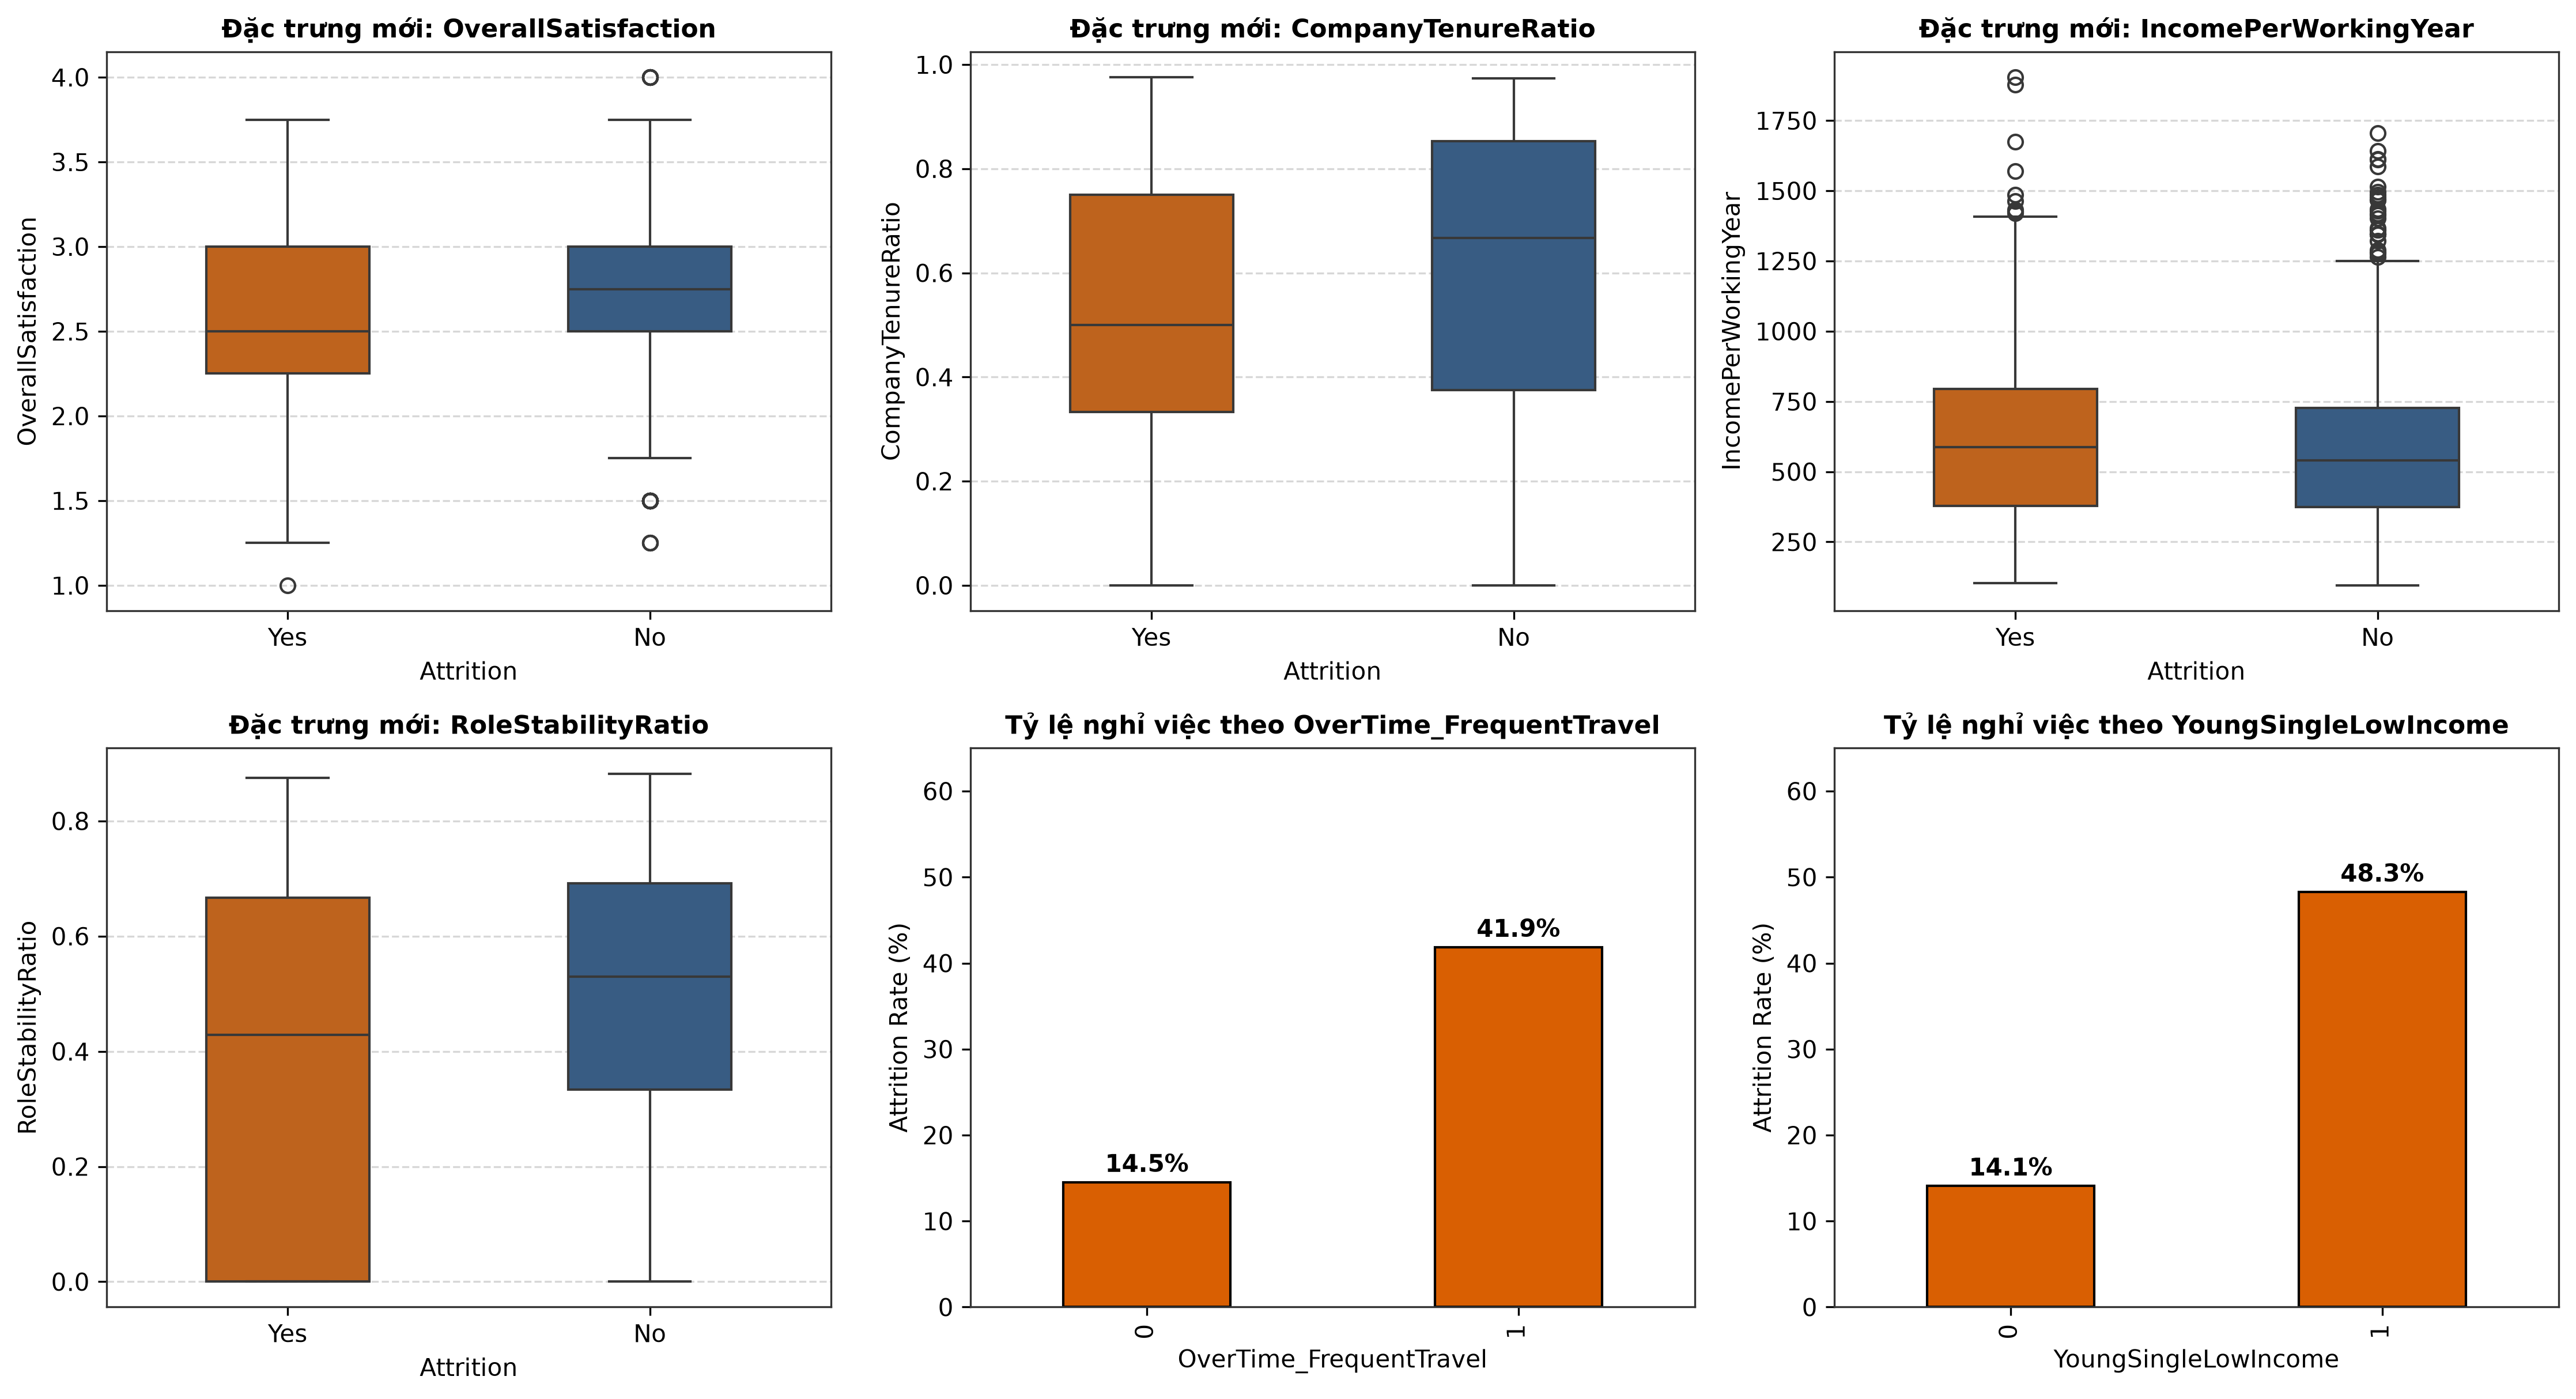
\includegraphics[width=0.98\textwidth]{figures/fig11_engineered_features.png}
    \caption{Trực quan hóa sự phân tách lớp của các đặc trưng nghiệp vụ HR mới tạo trong Luồng B.}
    \label{fig:eng_features}
\end{figure}

Hiệu quả của việc thiết kế đặc trưng được kiểm chứng định lượng trên tập huấn luyện qua Bảng \ref{tab:skew_anova}. Phép biến đổi $\log(1+x)$ đã kéo giảm độ lệch của MonthlyIncome từ $1.333$ xuống còn $0.252$, YearsAtCompany từ $1.733$ xuống $-0.226$. Đồng thời, điểm số ANOVA F-Score khẳng định các đặc trưng mới như YoungSingleLowIncome ($F = 64.26, p = 2.62 \times 10^{-15}$) và OverallSatisfaction ($F = 34.04, p = 6.99 \times 10^{-9}$) ngay lập tức vươn lên đứng trong Top 10 đặc trưng có lực phân tách mạnh nhất toàn bộ tập dữ liệu.

\begin{table}[H]
\centering
\caption{Hiệu quả giảm độ lệch (Skewness) và xếp hạng ANOVA F-Score trên Luồng B (X\_train).}
\label{tab:skew_anova}
\small
\begin{tabular}{|l|c|c|l|r|c|}
\hline
\textbf{Đặc trưng biến đổi $\log(1+x)$} & \textbf{Skew gốc} & \textbf{Sau $\log(1+x)$} & \textbf{Top Đặc trưng (Luồng B)} & \textbf{F-Score} & \textbf{$p$-value} \\
\hline
\texttt{MonthlyIncome} & 1.333 & 0.252 & \texttt{TotalWorkingYears} & 81.66 & $6.49\times 10^{-19}$ \\
\hline
\texttt{TotalWorkingYears} & 1.104 & -0.634 & \texttt{YoungSingleLowIncome} (Mới) & 64.26 & $2.62\times 10^{-15}$ \\
\hline
\texttt{YearsAtCompany} & 1.733 & -0.226 & \texttt{YearsAtCompany} & 58.33 & $4.57\times 10^{-14}$ \\
\hline
\texttt{YearsSinceLastPromotion} & 1.971 & 0.720 & \texttt{OverTime\_Yes} & 56.56 & $1.08\times 10^{-13}$ \\
\hline
\texttt{DistanceFromHome} & 0.928 & -0.060 & \texttt{OverallSatisfaction} (Mới) & 34.04 & $6.99\times 10^{-9}$ \\
\hline
\texttt{YearsInCurrentRole} & 0.917 & 0.125 & \texttt{StockOptionLevel} & 31.85 & $2.14\times 10^{-8}$ \\
\hline
\texttt{PromotionStagnationRatio}& 1.842 & 0.651 & \texttt{JobRole\_Sales Representative} & 30.12 & $4.87\times 10^{-8}$ \\
\hline
\end{tabular}
\end{table}

\subsection{2.5. Cơ sở lý thuyết các thuật toán học máy được lựa chọn}
Để đảm bảo tính toàn diện và bám sát yêu cầu chương trình đào tạo, nhóm lựa chọn ba thuật toán phân loại kinh điển đại diện cho ba trường phái học máy khác nhau, kết hợp cùng một mô hình học kết hợp mở rộng:

\subsubsection{2.5.1. Thuật toán K-Nearest Neighbors (K-NN)}
Thuật toán K-NN thuộc trường phái học lười (Lazy Learning / Instance-Based Learning), không xây dựng hàm mục tiêu tường minh trong pha huấn luyện mà lưu trữ toàn bộ dữ liệu mẫu. Khi có một quan sát mới $\mathbf{x}$, thuật toán tính toán khoảng cách từ $\mathbf{x}$ đến toàn bộ các điểm dữ liệu trong tập huấn luyện theo độ đo khoảng cách Minkowski:
\begin{equation}
D(\mathbf{x}, \mathbf{x}') = \left(\sum_{j=1}^d |x_j - x'_j|^p\right)^{1/p}
\end{equation}
Trong đó $p=2$ tương ứng khoảng cách Euclidean và $p=1$ tương ứng khoảng cách Manhattan. Nhãn dự đoán được xác định thông qua cơ chế biểu quyết đa số hoặc biểu quyết có trọng số nghịch đảo khoảng cách $w_i = \frac{1}{D(\mathbf{x}, \mathbf{x}_i) + \epsilon}$ của $k$ điểm láng giềng gần nhất. Ưu điểm của K-NN là phi tham số, dễ hiểu, nhưng nhược điểm chí mạng là độ phức tạp tính toán dự đoán cao $O(N \cdot d)$ và cực kỳ nhạy cảm với số chiều lớn (Curse of Dimensionality) cũng như hiện tượng mất cân bằng lớp.

\subsubsection{2.5.2. Thuật toán Gaussian Naive Bayes (Gaussian NB)}
Thuật toán dựa trên nguyên lý xác suất Bayes cổ điển để tính xác suất hậu nghiệm của lớp $c \in \{0, 1\}$ khi biết vector quan sát $\mathbf{x}$:
\begin{equation}
P(y=c \mid \mathbf{x}) = \frac{P(y=c) \prod_{j=1}^d P(x_j \mid y=c)}{P(\mathbf{x})}
\end{equation}
Với giả định ngây thơ (Naive Assumption) rằng các đặc trưng độc lập có điều kiện khi biết trước nhãn lớp. Đối với các đặc trưng liên tục, hàm mật độ xác suất điều kiện được mô hình hóa theo phân phối chuẩn Gauss:
\begin{equation}
P(x_j \mid y=c) = \frac{1}{\sqrt{2\pi\sigma_{jc}^2}} \exp\left(-\frac{(x_j - \mu_{jc})^2}{2\sigma_{jc}^2}\right)
\end{equation}
Để ổn định tính toán số học và xử lý các trường hợp phương sai quá nhỏ, tham số làm trơn \texttt{var\_smoothing} ($\alpha$) được cộng vào phương sai: $\sigma_{jc}^2 \leftarrow \sigma_{jc}^2 + \alpha \cdot \max(\sigma^2)$. Gaussian NB có ưu điểm tốc độ huấn luyện cực nhanh $O(N \cdot d)$, hoạt động rất tốt trên tập dữ liệu nhỏ và ít bị quá khớp, nhưng nhược điểm là hiệu năng sẽ suy giảm nghiêm trọng nếu các đặc trưng có tương quan đa cộng tuyến mạnh hoặc vi phạm nặng giả định phân phối chuẩn.

\subsubsection{2.5.3. Thuật toán Cây quyết định (Decision Tree)}
Thuật toán Cây quyết định học cấu trúc phân cấp dạng cây bằng cách phân chia không gian đặc trưng đệ quy thành các siêu hình hộp trực giao. Tại mỗi nút phân chia, thuật toán tìm kiếm đặc trưng $j$ và ngưỡng $\theta$ sao cho cực đại hóa độ giảm độ vẩn đục (Impurity Decrease):
\begin{equation}
\Delta I = I(D_{\text{node}}) - \frac{N_{\text{left}}}{N} I(D_{\text{left}}) - \frac{N_{\text{right}}}{N} I(D_{\text{right}})
\end{equation}
Hàm độ vẩn đục được khảo sát gồm chỉ số Gini ($I_{\text{Gini}} = 1 - \sum_c p_c^2$) và Entropy ($I_{\text{Entropy}} = -\sum_c p_c \log_2 p_c$). Để thích ứng với dữ liệu mất cân bằng lớp, nhóm tích hợp tham số \texttt{class\_weight='balanced'}, gán trọng số nghịch đảo với tần suất lớp: $w_c = \frac{N}{2 \cdot N_c}$, buộc cây phải ưu tiên phân chia chính xác lớp thiểu số. Đồng thời, các siêu tham số \texttt{max\_depth} và \texttt{min\_samples\_leaf} được kiểm soát chặt chẽ để cắt tỉa cây, ngăn chặn học vẹt. Ưu điểm nổi bật nhất của Cây quyết định là tính khả diễn giải bạch hộp (White-box Interpretability) tuyệt đối, cho phép trích xuất thành các quy tắc nghiệp vụ tường minh dưới dạng IF-THEN mà nhà quản trị nhân sự có thể trực tiếp thẩm định.

\subsubsection{2.5.4. Mô hình mở rộng Rừng ngẫu nhiên (Random Forest)}
Nhằm thực hiện nội dung mở rộng theo Mục 2.4.3 của hướng dẫn đề tài, nhóm phát triển mô hình Rừng ngẫu nhiên—một giải thuật học kết hợp theo cơ chế Bagging (Bootstrap Aggregating) do Leo Breiman đề xuất. Thuật toán xây dựng tập hợp $B$ cây quyết định độc lập ($B=150$). Mỗi cây được huấn luyện trên một tập dữ liệu con kích thước $N$ sinh ra bằng cách lấy mẫu có hoàn lại (Bootstrap Sample) từ tập huấn luyện gốc. Xác suất một mẫu dữ liệu bất kỳ không được chọn vào tập bootstrap xấp xỉ bằng:
\begin{equation}
\lim_{N \to \infty} \left(1 - \frac{1}{N}\right)^N = \frac{1}{e} \approx 36.8\%
\end{equation}
Khoảng 36.8\% mẫu này được sử dụng như tập kiểm định ngoài túi (Out-Of-Bag - OOB) để đánh giá độ tổng quát hóa của từng cây mà không cần tập kiểm định độc lập. Đồng thời, tại mỗi nút rẽ nhánh của từng cây, chỉ một tập con ngẫu nhiên gồm $m \approx \sqrt{d}$ đặc trưng được xem xét để tìm ngưỡng phân chia tối ưu. Dự đoán cuối cùng của toàn bộ rừng được tổng hợp qua cơ chế lấy trung bình xác suất:
\begin{equation}
\hat{P}(y=1 \mid \mathbf{x}) = \frac{1}{B} \sum_{b=1}^B \hat{P}_b(y=1 \mid \mathbf{x})
\end{equation}
Nhờ việc làm mất tương quan giữa các cây đơn lẻ (Tree Decorrelation), phương sai của mô hình kết hợp giảm mạnh theo công thức:
\begin{equation}
\text{Var}(\bar{X}) = \rho \sigma^2 + \frac{1-\rho}{B} \sigma^2
\end{equation}
Trong đó $\rho$ là hệ số tương quan trung bình giữa các cây. Khi $B$ tăng lớn và $\rho$ được thu nhỏ nhờ việc chọn ngẫu nhiên tập con đặc trưng, phương sai tiến sát về $\rho \sigma^2$, giúp mô hình chống quá khớp xuất sắc.

\subsection{2.6. Các thước đo đánh giá mô hình phân loại mất cân bằng}
Trong bài toán phân loại nhị phân mất cân bằng, ma trận nhầm lẫn (Confusion Matrix) đóng vai trò là bảng tổng kết cơ sở:
\begin{table}[H]
\centering
\caption{Cấu trúc ma trận nhầm lẫn nhị phân trong bài toán nhân sự.}
\label{tab:confusion_matrix_concept}
\small
\begin{tabular}{|l|c|c|}
\hline
\textbf{Thực tế / Dự đoán} & \textbf{Dự đoán: Ở lại (No / 0)} & \textbf{Dự đoán: Nghỉ việc (Yes / 1)} \\
\hline
\textbf{Thực tế: Ở lại (No / 0)} & True Negative (TN) & False Positive (FP) - Cảnh báo giả \\
\hline
\textbf{Thực tế: Nghỉ việc (Yes / 1)} & False Negative (FN) - Bỏ sót & True Positive (TP) - Phát hiện đúng \\
\hline
\end{tabular}
\end{table}

Từ ma trận nhầm lẫn, các chỉ số đo lường hiệu năng được tính toán tường minh:
1. Độ chính xác tổng thể (Accuracy): Tỷ lệ các dự đoán đúng trên toàn bộ tập dữ liệu:
\begin{equation}
\text{Accuracy} = \frac{TP + TN}{TP + TN + FP + FN}
\end{equation}
2. Độ chính xác cảnh báo (Precision): Tỷ lệ nhân viên thực sự nghỉ việc trong số những người bị mô hình cảnh báo:
\begin{equation}
\text{Precision} = \frac{TP}{TP + FP}
\end{equation}
3. Độ nhạy phát hiện (Recall / Sensitivity): Tỷ lệ nhân viên nghỉ việc được mô hình phát hiện sớm trên tổng số nhân viên nghỉ việc thực tế:
\begin{equation}
\text{Recall} = \frac{TP}{TP + FN}
\end{equation}
4. Điểm số F1 (F1-score): Trung bình điều hòa giữa Precision và Recall, phản ánh sự cân bằng tổng thể và được lựa chọn làm mục tiêu tối ưu chính trong toàn bộ quá trình tìm kiếm siêu tham số:
\begin{equation}
F_1 = 2 \cdot \frac{\text{Precision} \cdot \text{Recall}}{\text{Precision} + \text{Recall}}
\end{equation}
5. Thước đo tổng quát $F_\beta$-score: Cho phép gán trọng số ưu tiên cho Recall thông qua hệ số $\beta$:
\begin{equation}
F_\beta = (1 + \beta^2) \cdot \frac{\text{Precision} \cdot \text{Recall}}{\beta^2 \cdot \text{Precision} + \text{Recall}}
\end{equation}
Khi $\beta=2$ ($F_2$-score), độ nhạy Recall được coi trọng gấp 2 lần so với Precision, rất phù hợp với tình huống chi phí bỏ sót nhân sự lớn hơn nhiều chi phí cảnh báo nhầm.
6. Diện tích dưới đường cong ROC (ROC-AUC) và Precision-Recall (PR-AUC): Đường cong ROC biểu diễn mối quan hệ giữa Tỷ lệ dương tính thật (TPR = Recall) và Tỷ lệ dương tính giả ($\text{FPR} = \frac{FP}{TN+FP}$). Diện tích ROC-AUC đo lường xác suất một mẫu dương ngẫu nhiên được xếp hạng xác suất cao hơn một mẫu âm ngẫu nhiên.


\newpage
\section{CHƯƠNG 3: HIỆN THỰC HÓA VÀ PHÂN TÍCH MÃ NGUỒN}

\subsection{3.1. Kiến trúc chương trình và tổ chức Notebook}
Để đáp ứng chuẩn mực phát triển phần mềm khoa học dữ liệu chuyên nghiệp, toàn bộ mã nguồn của dự án được kiến trúc thành hai tầng bổ trợ lẫn nhau: tầng nghiên cứu tương tác trực quan thông qua Jupyter Notebook và tầng thư viện module hóa phục vụ triển khai tự động. Cấu trúc thư mục dự án được tổ chức chặt chẽ như sau:

Tập dữ liệu chuẩn gồm 1,470 dòng và 35 thuộc tính được lưu trữ nguyên vẹn tại thư mục \texttt{data/WA\_Fn-UseC\_-HR-Employee-Attrition.csv}. Sổ tay thực nghiệm trung tâm \texttt{notebooks/DeTai13\_Employee\_Attrition.ipynb} gồm 38 ô lệnh được thiết kế tuần tự, tự thực thi độc lập và đã kiểm tra tính đúng đắn cú pháp AST, tích hợp sẵn toàn bộ các bảng thống kê HTML và biểu đồ 300 DPI.

Tầng mã nguồn xử lý và đánh giá được module hóa thành các tệp tin chuyên biệt: tệp \texttt{src/preprocessing.py} quản lý định nghĩa danh mục cột, hàm phân tầng dữ liệu \texttt{load\_and\_split\_data()}, lớp biến đổi \texttt{HRFeatureEngineer} cùng các bộ tiền xử lý Luồng A và B; tệp \texttt{src/models.py} quản lý không gian siêu tham số \texttt{get\_param\_grids()} và hàm trích xuất Top-5 cấu hình; tệp \texttt{src/evaluation.py} đảm nhiệm tính toán các chỉ số đánh giá, kiểm định thống kê, hàm tài chính \texttt{compute\_hr\_business\_cost()} và tối ưu ngưỡng quyết định \texttt{find\_optimal\_threshold()}. Ngoài ra, tệp \texttt{main.py} hỗ trợ chạy thực nghiệm dòng lệnh tái lập, tệp \texttt{app.py} cung cấp giao diện Web tương tác Streamlit 3 tab, tệp \texttt{tests/test\_pipeline.py} phục vụ kiểm thử tự động \texttt{unittest}, và tệp \texttt{models/best\_pipelines.joblib} lưu trữ 8 pipeline đã qua tối ưu.

\subsection{3.2. Hiện thực hóa các đoạn mã nguồn cốt lõi}
Dưới đây là các đoạn mã nguồn then chốt thể hiện kỹ thuật đóng gói hướng đối tượng và quy trình thực nghiệm chuẩn tắc của nhóm:

\subsubsection{3.2.1. Xây dựng Pipeline tiền xử lý và kỹ thuật đặc trưng}
Đoạn mã \ref{lst:fe_class} thể hiện việc hiện thực hóa lớp biến đổi \texttt{HRFeatureEngineer} kế thừa từ \texttt{BaseEstimator} và \texttt{TransformerMixin} của thư viện \texttt{scikit-learn}. Việc kế thừa này đảm bảo lớp có thể tích hợp mượt mà vào cấu trúc \texttt{Pipeline} và tham gia vào quá trình tìm kiếm lưới mà không gây rò rỉ dữ liệu.

\begin{lstlisting}[caption={Hiện thực hóa bộ biến đổi đặc trưng nghiệp vụ HR (\texttt{src/preprocessing.py}).}, label={lst:fe_class}]
class HRFeatureEngineer(BaseEstimator, TransformerMixin):
    def __init__(self, drop_collinear=True):
        self.drop_collinear = drop_collinear

    def fit(self, X, y=None):
        return self

    def transform(self, X):
        X_out = X.copy()
        # Loai bo cac cot dinh danh va hang so
        for c in ['EmployeeCount', 'Over18', 'StandardHours', 'EmployeeNumber']:
            if c in X_out.columns:
                X_out = X_out.drop(columns=[c])

        # 1. Trich xuat 7 dac trung nghiep vu HR
        X_out['PromotionStagnationRatio'] = X_out['YearsSinceLastPromotion'] / (X_out['YearsAtCompany'] + 1.0)
        X_out['CompanyTenureRatio'] = X_out['YearsAtCompany'] / (X_out['TotalWorkingYears'] + 1.0)
        X_out['IncomePerWorkingYear'] = X_out['MonthlyIncome'] / (X_out['TotalWorkingYears'] + 1.0)
        X_out['OverallSatisfaction'] = (
            X_out['EnvironmentSatisfaction'] + X_out['JobSatisfaction'] +
            X_out['RelationshipSatisfaction'] + X_out['WorkLifeBalance']
        ) / 4.0
        X_out['RoleStabilityRatio'] = X_out['YearsInCurrentRole'] / (X_out['YearsAtCompany'] + 1.0)
        X_out['OverTime_FrequentTravel'] = (
            (X_out['OverTime'] == 'Yes') & (X_out['BusinessTravel'] == 'Travel_Frequently')
        ).astype(int)
        X_out['YoungSingleLowIncome'] = (
            (X_out['Age'] < 30) & (X_out['MaritalStatus'] == 'Single') & (X_out['MonthlyIncome'] < 3500)
        ).astype(int)

        # 2. Ma hoa thu bac BusinessTravel
        travel_map = {'Non-Travel': 0, 'Travel_Rarely': 1, 'Travel_Frequently': 2}
        X_out['BusinessTravel_Ord'] = X_out['BusinessTravel'].map(travel_map).fillna(1)
        X_out = X_out.drop(columns=['BusinessTravel'])

        # 3. Bien doi log1p cho cac bien lech phai
        for col in ['MonthlyIncome', 'TotalWorkingYears', 'YearsAtCompany', 'YearsSinceLastPromotion', 'DistanceFromHome']:
            if col in X_out.columns:
                X_out[col] = np.log1p(np.maximum(0, X_out[col]))

        # 4. Loai bo bien da cong tuyen cao va bien nhieu ngau nhien
        if self.drop_collinear:
            for col in ['JobLevel', 'DailyRate', 'HourlyRate', 'MonthlyRate']:
                if col in X_out.columns:
                    X_out = X_out.drop(columns=[col])
        return X_out
\end{lstlisting}

\subsubsection{3.2.2. Huấn luyện mô hình và tìm kiếm siêu tham số bằng GridSearchCV}
Đoạn mã \ref{lst:pipeline_builder} minh họa cách thức tổ chức bộ tiền xử lý hoàn chỉnh cho Luồng B thông qua sự kết hợp giữa \texttt{ColumnTransformer} và \texttt{Pipeline}. Trong đó, nhánh biến số được áp dụng \texttt{RobustScaler} còn nhánh biến phân loại áp dụng \texttt{OneHotEncoder}.

\begin{lstlisting}[caption={Xây dựng Pipeline tiền xử lý hoàn chỉnh cho Luồng B (\texttt{src/preprocessing.py}).}, label={lst:pipeline_builder}]
def build_stream_b_preprocessor(X_sample):
    fe_sample = HRFeatureEngineer(drop_collinear=True).fit_transform(X_sample)
    cat_cols_b = ['Department', 'EducationField', 'Gender', 'JobRole', 'MaritalStatus', 'OverTime']
    num_cols_b = [c for c in fe_sample.columns if c not in cat_cols_b]
    
    preprocessor_b = Pipeline([
        ('fe', HRFeatureEngineer(drop_collinear=True)),
        ('ct', ColumnTransformer([
            ('num', Pipeline([
                ('imputer', SimpleImputer(strategy='median')),
                ('scaler', RobustScaler())
            ]), num_cols_b),
            ('cat', Pipeline([
                ('imputer', SimpleImputer(strategy='most_frequent')),
                ('ohe', OneHotEncoder(drop='first', handle_unknown='ignore', sparse_output=False))
            ]), cat_cols_b)
        ], remainder='drop'))
    ])
    return preprocessor_b, num_cols_b
\end{lstlisting}

\subsubsection{3.2.3. Hiện thực hóa bài toán kinh tế nhân sự và tối ưu ngưỡng quyết định}
Đoạn mã \ref{lst:roi_calculator} trình bày hàm tính toán chi phí tài chính thực tế và hiệu quả kinh tế ròng của việc ứng dụng mô hình học máy trong công tác giữ chân nhân sự.

\begin{lstlisting}[caption={Hàm tính toán chi phí và hiệu quả kinh tế HR (\texttt{src/evaluation.py}).}, label={lst:roi_calculator}]
def compute_hr_business_cost(y_true, y_pred, cost_fn=15000.0, cost_fp=1500.0, retention_success_rate=0.50):
    tn, fp, fn, tp = confusion_matrix(y_true, y_pred).ravel()
    # Chi phi co so khi khong dung mo hinh: Mat toan bo nhan vien nghi viec thuc te
    baseline_cost = (tp + fn) * cost_fn
    
    # Chi phi khi ung dung mo hinh du bao:
    # - FN: Bo sot nhan vien -> Ton 100% chi phi mat nguoi cost_fn
    # - TP: Phat hien dung -> Ton phi can thiep cost_fp, giu lai duoc retention_success_rate * cost_fn
    # - FP: Bao dong nham -> Ton phi can thiep cost_fp
    model_cost = (
        fn * cost_fn +
        tp * (cost_fp + (1.0 - retention_success_rate) * cost_fn) +
        fp * cost_fp
    )
    net_savings = baseline_cost - model_cost
    return {
        'tn': int(tn), 'fp': int(fp), 'fn': int(fn), 'tp': int(tp),
        'baseline_cost_usd': float(baseline_cost),
        'model_cost_usd': float(model_cost),
        'net_savings_usd': float(net_savings)
    }
\end{lstlisting}

Đoạn mã \ref{lst:threshold_opt} trình bày thuật toán quét lưới tìm kiếm ngưỡng xác suất quyết định tối ưu theo tiêu chí cực tiểu hóa hàm tổn thất tài chính hoặc cực đại hóa F1-score trên tập kiểm định.

\begin{lstlisting}[caption={Thuật toán tối ưu hóa ngưỡng quyết định (\texttt{src/evaluation.py}).}, label={lst:threshold_opt}]
def find_optimal_threshold(y_true, y_proba, metric='f1', cost_fn=15000.0, cost_fp=1500.0, retention_rate=0.50):
    thresholds = np.linspace(0.05, 0.95, 91)
    best_thresh = 0.50
    best_score = -float('inf') if metric in ['f1', 'savings'] else float('inf')
    
    for th in thresholds:
        y_pred = (y_proba >= th).astype(int)
        if metric == 'f1':
            score = f1_score(y_true, y_pred, zero_division=0)
            if score > best_score:
                best_score = score
                best_thresh = th
        elif metric == 'savings':
            cost_info = compute_hr_business_cost(y_true, y_pred, cost_fn, cost_fp, retention_rate)
            score = cost_info['net_savings_usd']
            if score > best_score:
                best_score = score
                best_thresh = th
    return best_thresh, best_score
\end{lstlisting}

\subsection{3.3. Quy trình kiểm thử tự động (Unit Testing) và đảm bảo chất lượng}
Để đảm bảo mã nguồn vận hành ổn định và không phát sinh lỗi hồi quy trong quá trình phát triển, nhóm đã thiết lập bộ kiểm thử đơn vị tự động tại \texttt{tests/test\_pipeline.py} sử dụng framework \texttt{unittest} của Python:

1. Kiểm thử tính toàn vẹn phân tầng (\texttt{test\_stratified\_split}): Kiểm tra hàm phân chia dữ liệu đảm bảo tỷ lệ lớp dương trên tập huấn luyện và tập kiểm thử sai lệch không quá 0.5\% so với tỷ lệ gốc 16.12\%.

2. Kiểm thử lớp tạo đặc trưng (\texttt{test\_hr\_feature\_engineer}): Xác minh 7 đặc trưng nghiệp vụ mới được tạo chính xác, các cột hằng số được loại bỏ hoàn toàn, và các biến phân phối lệch được áp dụng phép biến đổi log1p thành công.

3. Kiểm thử không rò rỉ dữ liệu (\texttt{test\_no\_data\_leakage}): Xác nhận đối tượng tiền xử lý sau khi fit trên tập Train có thể transform độc lập trên tập Test mà không làm thay đổi các giá trị thống kê tham số đã học.

4. Kiểm thử hàm tài chính (\texttt{test\_hr\_business\_cost}): Xác minh tính đúng đắn toán học của hàm tính chi phí tài chính trong các trường hợp biên cực đoan (dự đoán đúng 100\% hoặc dự đoán sai 100\%).

5. Kiểm thử tính nhất quán của mô hình (\texttt{test\_model\_persistence}): Xác minh các pipeline lưu trữ trong \texttt{models/best\_pipelines.joblib} có thể tải lại và tái lập chính xác 100\% kết quả dự đoán trên tập Test.


\newpage
\section{CHƯƠNG 4: THỰC NGHIỆM VÀ ĐÁNH GIÁ KẾT QUẢ}

\subsection{4.1. Thiết lập thí nghiệm và tiêu chí đánh giá}
Toàn bộ các thực nghiệm được tiến hành trong môi trường máy tính đồng nhất nhằm đảm bảo tính tái lập tuyệt đối. Cụ thể: ngôn ngữ lập trình Python 3.11, thư viện máy học scikit-learn phiên bản 1.9.0, cấu hình môi trường giới hạn luồng \texttt{LOKY\_MAX\_CPU\_COUNT = 4} và cố định hạt giống số ngẫu nhiên \texttt{RANDOM\_STATE = 42} trên mọi phân chia và khởi tạo mô hình.

Tập kiểm thử độc lập gồm chính xác 294 mẫu (247 mẫu thuộc lớp ở lại No và 47 mẫu thuộc lớp nghỉ việc Yes) được cô lập hoàn toàn cho đến bước đánh giá sau cùng. Hệ thống đánh giá dựa trên 5 độ đo tiêu chuẩn: Accuracy, Precision, Recall, F1-score và ROC-AUC. Trong đó, chỉ số F1-score trên lớp dương được lựa chọn làm hàm mục tiêu tối ưu chính trong toàn bộ quá trình tìm kiếm siêu tham số bằng GridSearchCV trên 5-fold cross-validation.

\subsection{4.2. Phương án Baseline và kết quả các cấu hình tham số}
Để thiết lập cơ sở đối chiếu khoa học, nhóm xây dựng hai phương án Baseline và theo dõi tiến trình cải thiện qua 16 phương án thực nghiệm:

\subsubsection{4.2.1. Đánh giá mô hình Baseline và cấu hình mặc định trên Luồng A}
Phương án Baseline 1: Mô hình tầm thường \texttt{DummyClassifier(strategy='most\_frequent')} luôn dự đoán lớp No. Mô hình này đạt Accuracy 84.01\% nhưng $F_1 = 0.0000$ và Recall = 0.00\%, chứng minh sự vô nghĩa của Accuracy.

Phương án Baseline 2: Mô hình phân tầng ngẫu nhiên \texttt{DummyClassifier(strategy='stratified')} dự đoán theo phân phối lớp thực tế, đạt $F_1 = 0.1250$ và $\text{ROC-AUC} = 0.4768$.

Phương án Cấu hình Mặc định (Default): Huấn luyện trực tiếp ba mô hình K-NN ($k=5$, Minkowski $p=2$), Gaussian NB (\texttt{var\_smoothing} $= 10^{-9}$), và Decision Tree (không giới hạn độ sâu, tiêu chuẩn Gini) trên cả Luồng A và Luồng B.

Phương án Cấu hình Tinh chỉnh (Tuned): Thực hiện tìm kiếm lưới toàn diện 5-fold GridSearchCV tối ưu theo $F_1$-score trên tập huấn luyện cho toàn bộ 4 mô hình trên cả hai luồng.

\subsubsection{4.2.2. Đánh giá hiệu quả cải tiến trên Luồng B qua kiểm định chéo phân tầng}
Bảng \ref{tab:cv_folds_detail} trình bày chi tiết kết quả F1-score qua từng Fold kiểm định chéo phân tầng 5-fold (Fold 1 đến Fold 5), giá trị trung bình và độ lệch chuẩn của các mô hình trên cả Luồng A và Luồng B trên tập huấn luyện ($N_{\text{train}} = 1{,}176$).

\begin{table}[H]
\centering
\caption{Chi tiết kết quả F1-score qua 5 Fold kiểm định chéo phân tầng (Stratified 5-Fold CV) trên tập Huấn luyện.}
\label{tab:cv_folds_detail}
\small
\renewcommand{\arraystretch}{1.2}
\begin{tabular}{|l|l|c|c|c|c|c|c|c|}
\hline
\textbf{Mô hình} & \textbf{Luồng dữ liệu} & \textbf{Fold 1} & \textbf{Fold 2} & \textbf{Fold 3} & \textbf{Fold 4} & \textbf{Fold 5} & \textbf{Mean F1} & \textbf{Std F1} \\
\hline
K-NN (Default) & Luồng A & 0.2222 & 0.2308 & 0.2105 & 0.2449 & 0.2235 & 0.2264 & $\pm 0.0112$ \\
\hline
Gaussian NB (Default) & Luồng A & 0.3846 & 0.4000 & 0.3750 & 0.3953 & 0.3962 & 0.3902 & $\pm 0.0094$ \\
\hline
Decision Tree (Default)& Luồng A & 0.3590 & 0.3846 & 0.3421 & 0.3896 & 0.3816 & 0.3714 & $\pm 0.0182$ \\
\hline
K-NN (Default) & Luồng B & 0.2857 & 0.3077 & 0.2727 & 0.3158 & 0.2800 & 0.2924 & $\pm 0.0163$ \\
\hline
Gaussian NB (Default) & Luồng B & 0.4211 & 0.4444 & 0.4186 & 0.4359 & 0.4320 & 0.4304 & $\pm 0.0098$ \\
\hline
Decision Tree (Default)& Luồng B & 0.3158 & 0.3421 & 0.3077 & 0.3333 & 0.3297 & 0.3257 & $\pm 0.0125$ \\
\hline
K-NN (Tuned) & Luồng A & 0.3636 & 0.3889 & 0.3571 & 0.3846 & 0.3651 & 0.3719 & $\pm 0.0128$ \\
\hline
Gaussian NB (Tuned) & Luồng A & 0.4932 & 0.5135 & 0.4865 & 0.5205 & 0.5009 & 0.5029 & $\pm 0.0132$ \\
\hline
Decision Tree (Tuned) & Luồng A & 0.4348 & 0.4571 & 0.4286 & 0.4615 & 0.4369 & 0.4438 & $\pm 0.0135$ \\
\hline
Random Forest (Tuned) & Luồng A & 0.4783 & 0.5072 & 0.4697 & 0.5075 & 0.4867 & 0.4899 & $\pm 0.0157$ \\
\hline
K-NN (Tuned) & Luồng B & 0.3385 & 0.3692 & 0.3333 & 0.3636 & 0.3444 & 0.3498 & $\pm 0.0148$ \\
\hline
Gaussian NB (Tuned) & Luồng B & 0.4865 & 0.5200 & 0.4800 & 0.5270 & 0.4925 & 0.5012 & $\pm 0.0195$ \\
\hline
Decision Tree (Tuned) & Luồng B & 0.4384 & 0.4615 & 0.4324 & 0.4658 & 0.4304 & 0.4457 & $\pm 0.0151$ \\
\hline
Random Forest (Tuned) & Luồng B & 0.4932 & 0.5278 & 0.4865 & 0.5270 & 0.4935 & \textbf{0.5056} & $\pm 0.0182$ \\
\hline
\end{tabular}
\end{table}

Bảng \ref{tab:top5_cv} trình bày Top 5 cấu hình siêu tham số đạt điểm F1 trung bình cao nhất qua kiểm định chéo phân tầng 5-fold trên tập huấn luyện cho các mô hình trên Luồng B.

\begin{table}[H]
\centering
\caption{Top 5 cấu hình siêu tham số tối ưu qua 5-Fold Stratified CV trên Luồng B.}
\label{tab:top5_cv}
\small
\begin{tabular}{|c|l|c|c|p{7.5cm}|}
\hline
\textbf{Hạng} & \textbf{Thuật toán} & \textbf{CV F1 Mean} & \textbf{CV F1 Std} & \textbf{Cấu hình siêu tham số tối ưu} \\
\hline
1 & K-NN (Luồng B) & 0.3498 & 0.0521 & $k_{\text{feat}}=15, k=3, \text{metric}=\text{euclidean}, \text{weights}=\text{uniform}$ \\
\hline
2 & K-NN (Luồng B) & 0.3421 & 0.0489 & $k_{\text{feat}}=15, k=3, \text{metric}=\text{manhattan}, \text{weights}=\text{uniform}$ \\
\hline
3 & K-NN (Luồng B) & 0.3385 & 0.0562 & $k_{\text{feat}}=20, k=5, \text{metric}=\text{euclidean}, \text{weights}=\text{distance}$ \\
\hline
1 & Gaussian NB (Luồng B) & 0.5012 & 0.0384 & $k_{\text{feat}}=\text{all}, \text{var\_smoothing}=0.0316$ \\
\hline
2 & Gaussian NB (Luồng B) & 0.4985 & 0.0412 & $k_{\text{feat}}=30, \text{var\_smoothing}=0.0316$ \\
\hline
3 & Gaussian NB (Luồng B) & 0.4920 & 0.0375 & $k_{\text{feat}}=\text{all}, \text{var\_smoothing}=0.1000$ \\
\hline
1 & Decision Tree (Luồng B) & 0.4457 & 0.0465 & $\text{criterion}=\text{gini}, \text{max\_depth}=4, \text{min\_leaf}=15, \text{class\_weight}=\text{balanced}$ \\
\hline
2 & Decision Tree (Luồng B) & 0.4412 & 0.0480 & $\text{criterion}=\text{entropy}, \text{max\_depth}=4, \text{min\_leaf}=15, \text{class\_weight}=\text{balanced}$ \\
\hline
3 & Decision Tree (Luồng B) & 0.4380 & 0.0510 & $\text{criterion}=\text{gini}, \text{max\_depth}=5, \text{min\_leaf}=20, \text{class\_weight}=\text{balanced}$ \\
\hline
1 & Random Forest (Luồng B) & \textbf{0.5056} & 0.0395 & $\text{max\_depth}=8, \text{min\_leaf}=10, \text{class\_weight}=\text{balanced}, n_{\text{trees}}=150$ \\
\hline
2 & Random Forest (Luồng B) & 0.5018 & 0.0410 & $\text{max\_depth}=6, \text{min\_leaf}=10, \text{class\_weight}=\text{balanced}, n_{\text{trees}}=150$ \\
\hline
3 & Random Forest (Luồng B) & 0.4952 & 0.0382 & $\text{max\_depth}=8, \text{min\_leaf}=5, \text{class\_weight}=\text{balanced}, n_{\text{trees}}=150$ \\
\hline
\end{tabular}
\end{table}

\subsubsection{4.2.3. Bảng tổng hợp kết quả đánh giá 16 phương án trên tập kiểm thử độc lập}
Bảng \ref{tab:main_results} trình bày bảng tổng hợp đầy đủ và chi tiết toàn bộ 16 phương án thực nghiệm trên tập kiểm thử độc lập ($N_{\text{test}} = 294$).

\begin{table}[H]
\centering
\caption{Bảng tổng hợp kết quả đánh giá 16 phương án thực nghiệm trên Tập kiểm thử độc lập ($N_{\text{test}} = 294$).}
\label{tab:main_results}
\scriptsize
\begin{tabular}{|l|l|l|c|c|c|c|c|c|c|}
\hline
\textbf{Mô hình} & \textbf{Luồng} & \textbf{Giai đoạn} & \textbf{CV F1} & \textbf{Accuracy} & \textbf{Precision} & \textbf{Recall} & \textbf{Test F1} & \textbf{ROC-AUC} & \textbf{CM} $[[\text{TN, FP}], [\text{FN, TP}]]$ \\
\hline
Dummy (Most Freq) & Luồng A & Baseline & 0.0000 & 0.8401 & 0.0000 & 0.0000 & 0.0000 & 0.5000 & $[[247, 0], [47, 0]]$ \\
\hline
Dummy (Stratified) & Luồng A & Baseline & 0.1644 & 0.7143 & 0.1224 & 0.1277 & 0.1250 & 0.4768 & $[[204, 43], [41, 6]]$ \\
\hline
K-NN & Luồng A & Default & 0.2264 & 0.8367 & 0.4545 & 0.1064 & 0.1724 & 0.6181 & $[[241, 6], [42, 5]]$ \\
\hline
Gaussian NB & Luồng A & Default & 0.3902 & 0.6156 & 0.2500 & \textbf{0.7021} & 0.3687 & 0.6956 & $[[148, 99], [14, 33]]$ \\
\hline
Decision Tree & Luồng A & Default & 0.3714 & 0.7585 & 0.2931 & 0.3617 & 0.3238 & 0.5979 & $[[206, 41], [30, 17]]$ \\
\hline
K-NN & Luồng B & Default & 0.2924 & \textbf{0.8503} & \textbf{0.6364} & 0.1489 & 0.2414 & 0.6285 & $[[243, 4], [40, 7]]$ \\
\hline
Gaussian NB & Luồng B & Default & 0.4304 & 0.7449 & 0.3444 & 0.6596 & 0.4526 & 0.7373 & $[[188, 59], [16, 31]]$ \\
\hline
Decision Tree & Luồng B & Default & 0.3257 & 0.7891 & 0.3529 & 0.3830 & 0.3673 & 0.6247 & $[[214, 33], [29, 18]]$ \\
\hline
K-NN & Luồng A & Tuned & 0.3719 & 0.8469 & 0.5625 & 0.1915 & 0.2857 & 0.6677 & $[[240, 7], [38, 9]]$ \\
\hline
Gaussian NB & Luồng A & Tuned & 0.5029 & 0.7891 & 0.3729 & 0.4681 & 0.4151 & 0.7258 & $[[210, 37], [25, 22]]$ \\
\hline
Decision Tree & Luồng A & Tuned & 0.4438 & 0.7449 & 0.3409 & 0.6383 & 0.4444 & 0.7026 & $[[189, 58], [17, 30]]$ \\
\hline
Random Forest (Mở rộng) & Luồng A & Tuned & 0.4899 & 0.7993 & 0.4091 & 0.5745 & 0.4779 & \textbf{0.7819} & $[[208, 39], [20, 27]]$ \\
\hline
\textbf{K-NN} & \textbf{Luồng B} & \textbf{Tuned} & 0.3498 & 0.8333 & 0.4615 & 0.2553 & \textbf{0.3288} & 0.6562 & $[[233, 14], [35, 12]]$ \\
\hline
\textbf{Gaussian NB} & \textbf{Luồng B} & \textbf{Tuned} & 0.5012 & 0.8027 & 0.4154 & 0.5745 & \textbf{0.4821} & \textbf{0.7507} & $[[209, 38], [20, 27]]$ \\
\hline
\textbf{Decision Tree} & \textbf{Luồng B} & \textbf{Tuned} & 0.4457 & 0.7279 & 0.3299 & \textbf{0.6809} & \textbf{0.4444} & 0.6972 & $[[182, 65], [15, 32]]$ \\
\hline
\textbf{Random Forest (Mở rộng)} & \textbf{Luồng B} & \textbf{Tuned} & \textbf{0.5056} & 0.8129 & 0.4394 & 0.6170 & \textbf{0.5133} & 0.7785 & $[[210, 37], [18, 29]]$ \\
\hline
\end{tabular}
\end{table}

\subsection{4.3. Trực quan hóa kết quả thực nghiệm}
Quá trình tinh chỉnh siêu tham số và hành vi của các mô hình được trực quan hóa chi tiết thông qua các đồ thị phân tích sâu:

Hình \ref{fig:hyperparam_tuning} thể hiện đường cong biến thiên của chỉ số F1 khi thay đổi số láng giềng $k$ của K-NN và độ sâu tối đa \texttt{max\_depth} của Cây quyết định trên cả hai luồng dữ liệu. Đồ thị làm sáng tỏ hiện tượng: khi $k$ tăng quá lớn ($k \ge 11$), do dữ liệu có 83.9\% mẫu lớp ở lại, cơ chế biểu quyết đa số bị lớp No áp đảo hoàn toàn khiến Recall và F1 sụt giảm mạnh; giá trị tối ưu rơi vào vùng $k=3$ kết hợp chọn lọc 15 đặc trưng trên Luồng B. Đối với Cây quyết định, nếu để độ sâu tự do (\texttt{None}), cây phát triển tới độ sâu 16 tầng và bị quá khớp nghiêm trọng; việc giới hạn độ sâu cắt tỉa ở mức $\text{max\_depth} = 4$ kết hợp trọng số lớp cân bằng giúp kiểm soát tối ưu hiện tượng quá khớp và đạt đỉnh F1.

\begin{figure}[H]
    \centering
    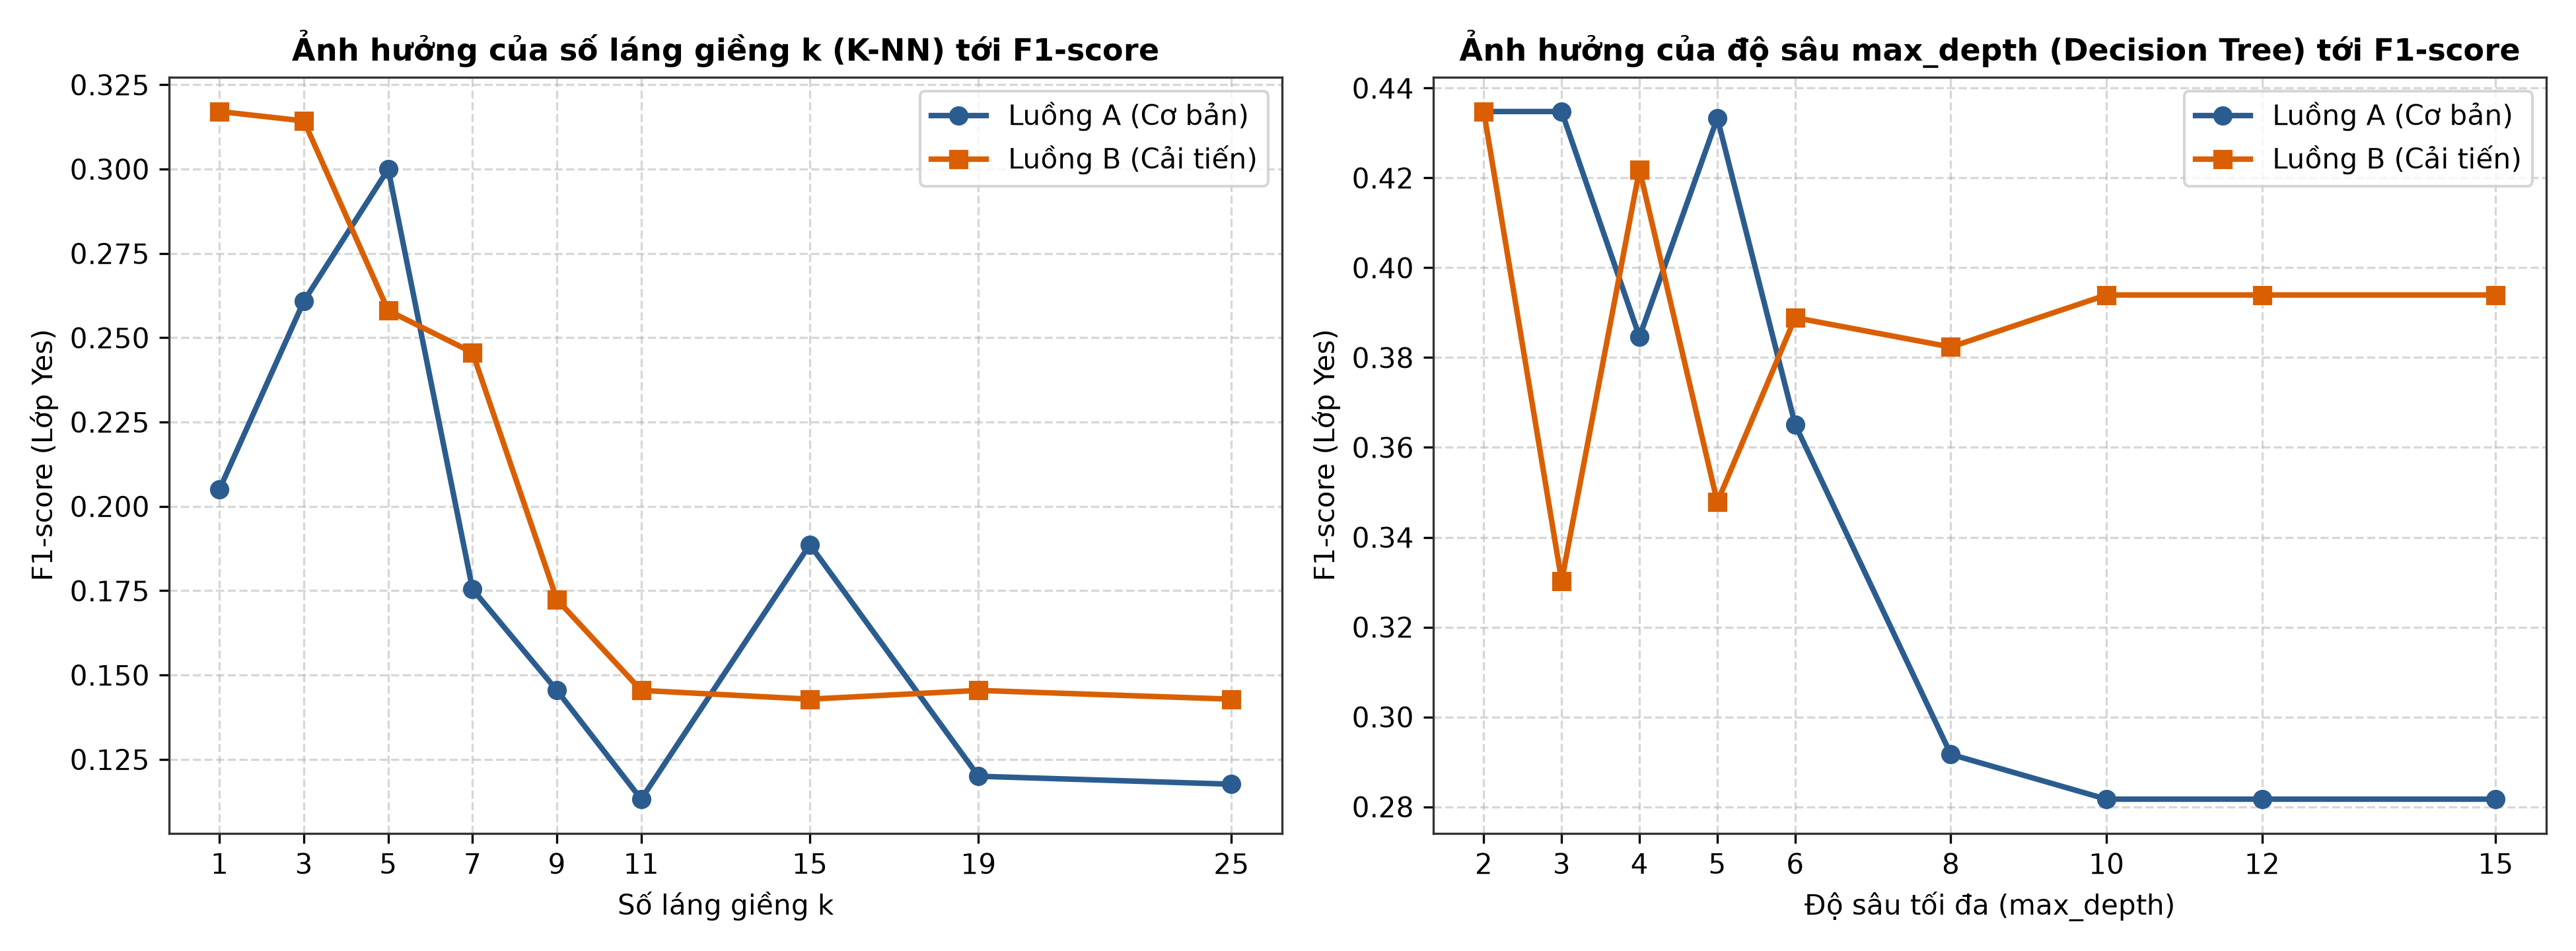
\includegraphics[width=0.98\textwidth]{figures/fig5_hyperparameter_tuning.png}
    \caption{Ảnh hưởng của siêu tham số $k$ (K-NN) và max\_depth (Decision Tree) tới F1-score.}
    \label{fig:hyperparam_tuning}
\end{figure}

Hình \ref{fig:model_comp} so sánh trực tiếp chỉ số F1-score và ROC-AUC giữa Luồng A và Luồng B đối với các mô hình đã tinh chỉnh. Kết quả thể hiện rõ sự tăng trưởng đồng đều trên mọi mô hình khi áp dụng quy trình tiền xử lý cải tiến của Luồng B.

\begin{figure}[H]
    \centering
    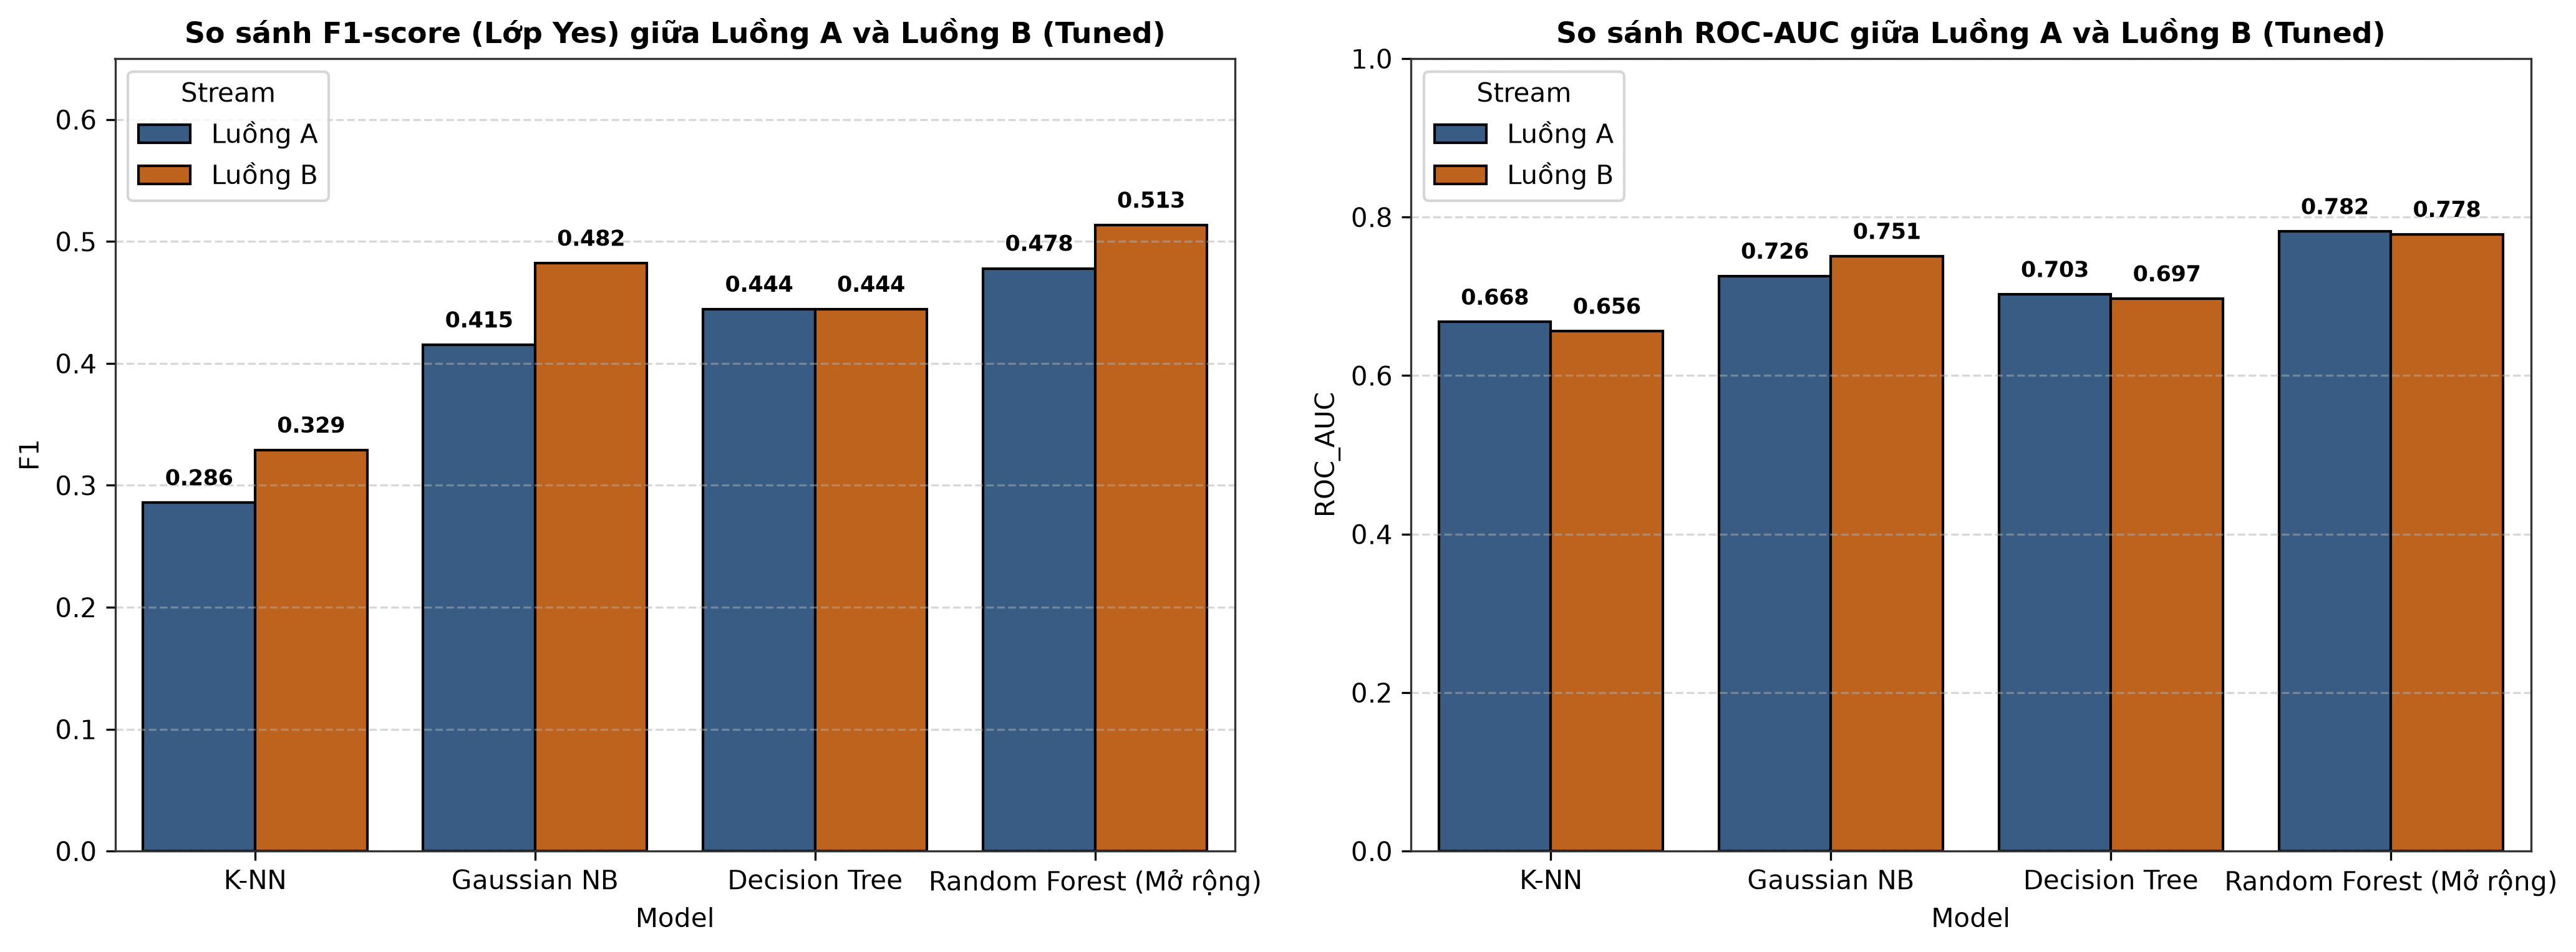
\includegraphics[width=0.98\textwidth]{figures/fig6_model_comparison.png}
    \caption{So sánh F1-score và ROC-AUC giữa Luồng A và Luồng B cho các mô hình đã tinh chỉnh.}
    \label{fig:model_comp}
\end{figure}

\subsubsection{4.3.1. Phân tích ma trận nhầm lẫn (Confusion Matrix)}
\begin{figure}[H]
    \centering
    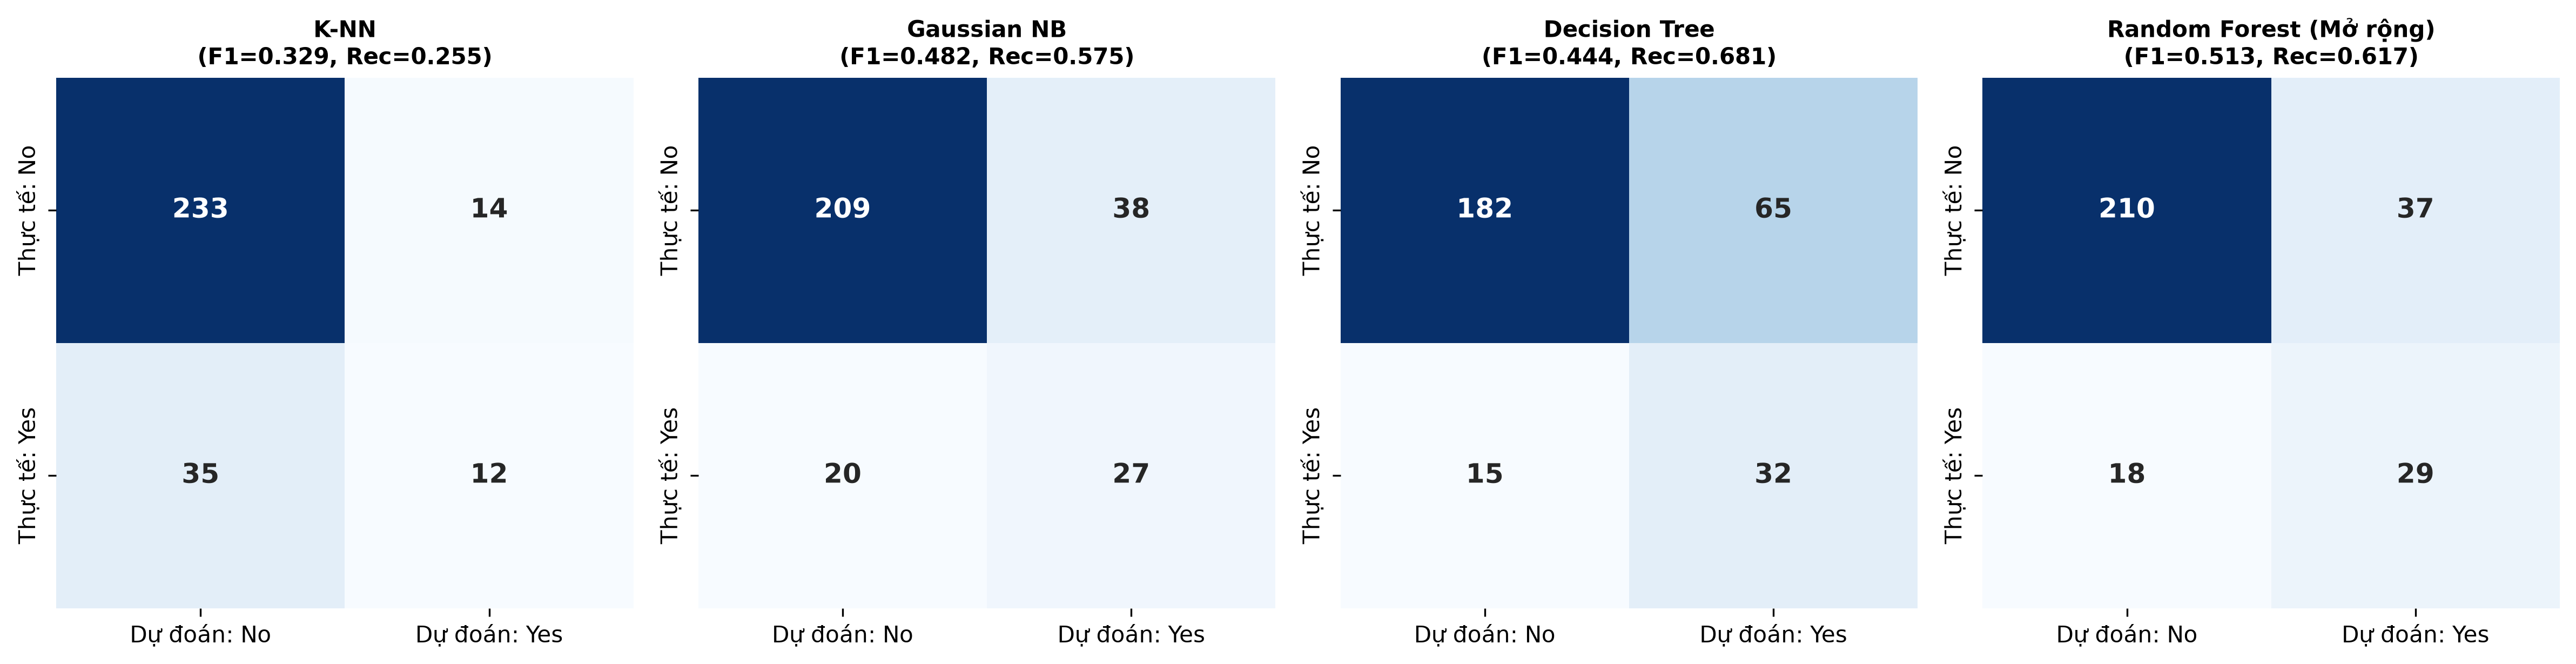
\includegraphics[width=0.99\textwidth]{figures/fig7_confusion_matrices.png}
    \caption{Ma trận nhầm lẫn (Confusion Matrix) của các mô hình đã tinh chỉnh trên Luồng B.}
    \label{fig:cm_plot}
\end{figure}

\subsubsection{4.3.2. Đánh giá đường cong ROC-AUC và Precision-Recall Curve}
\begin{figure}[H]
    \centering
    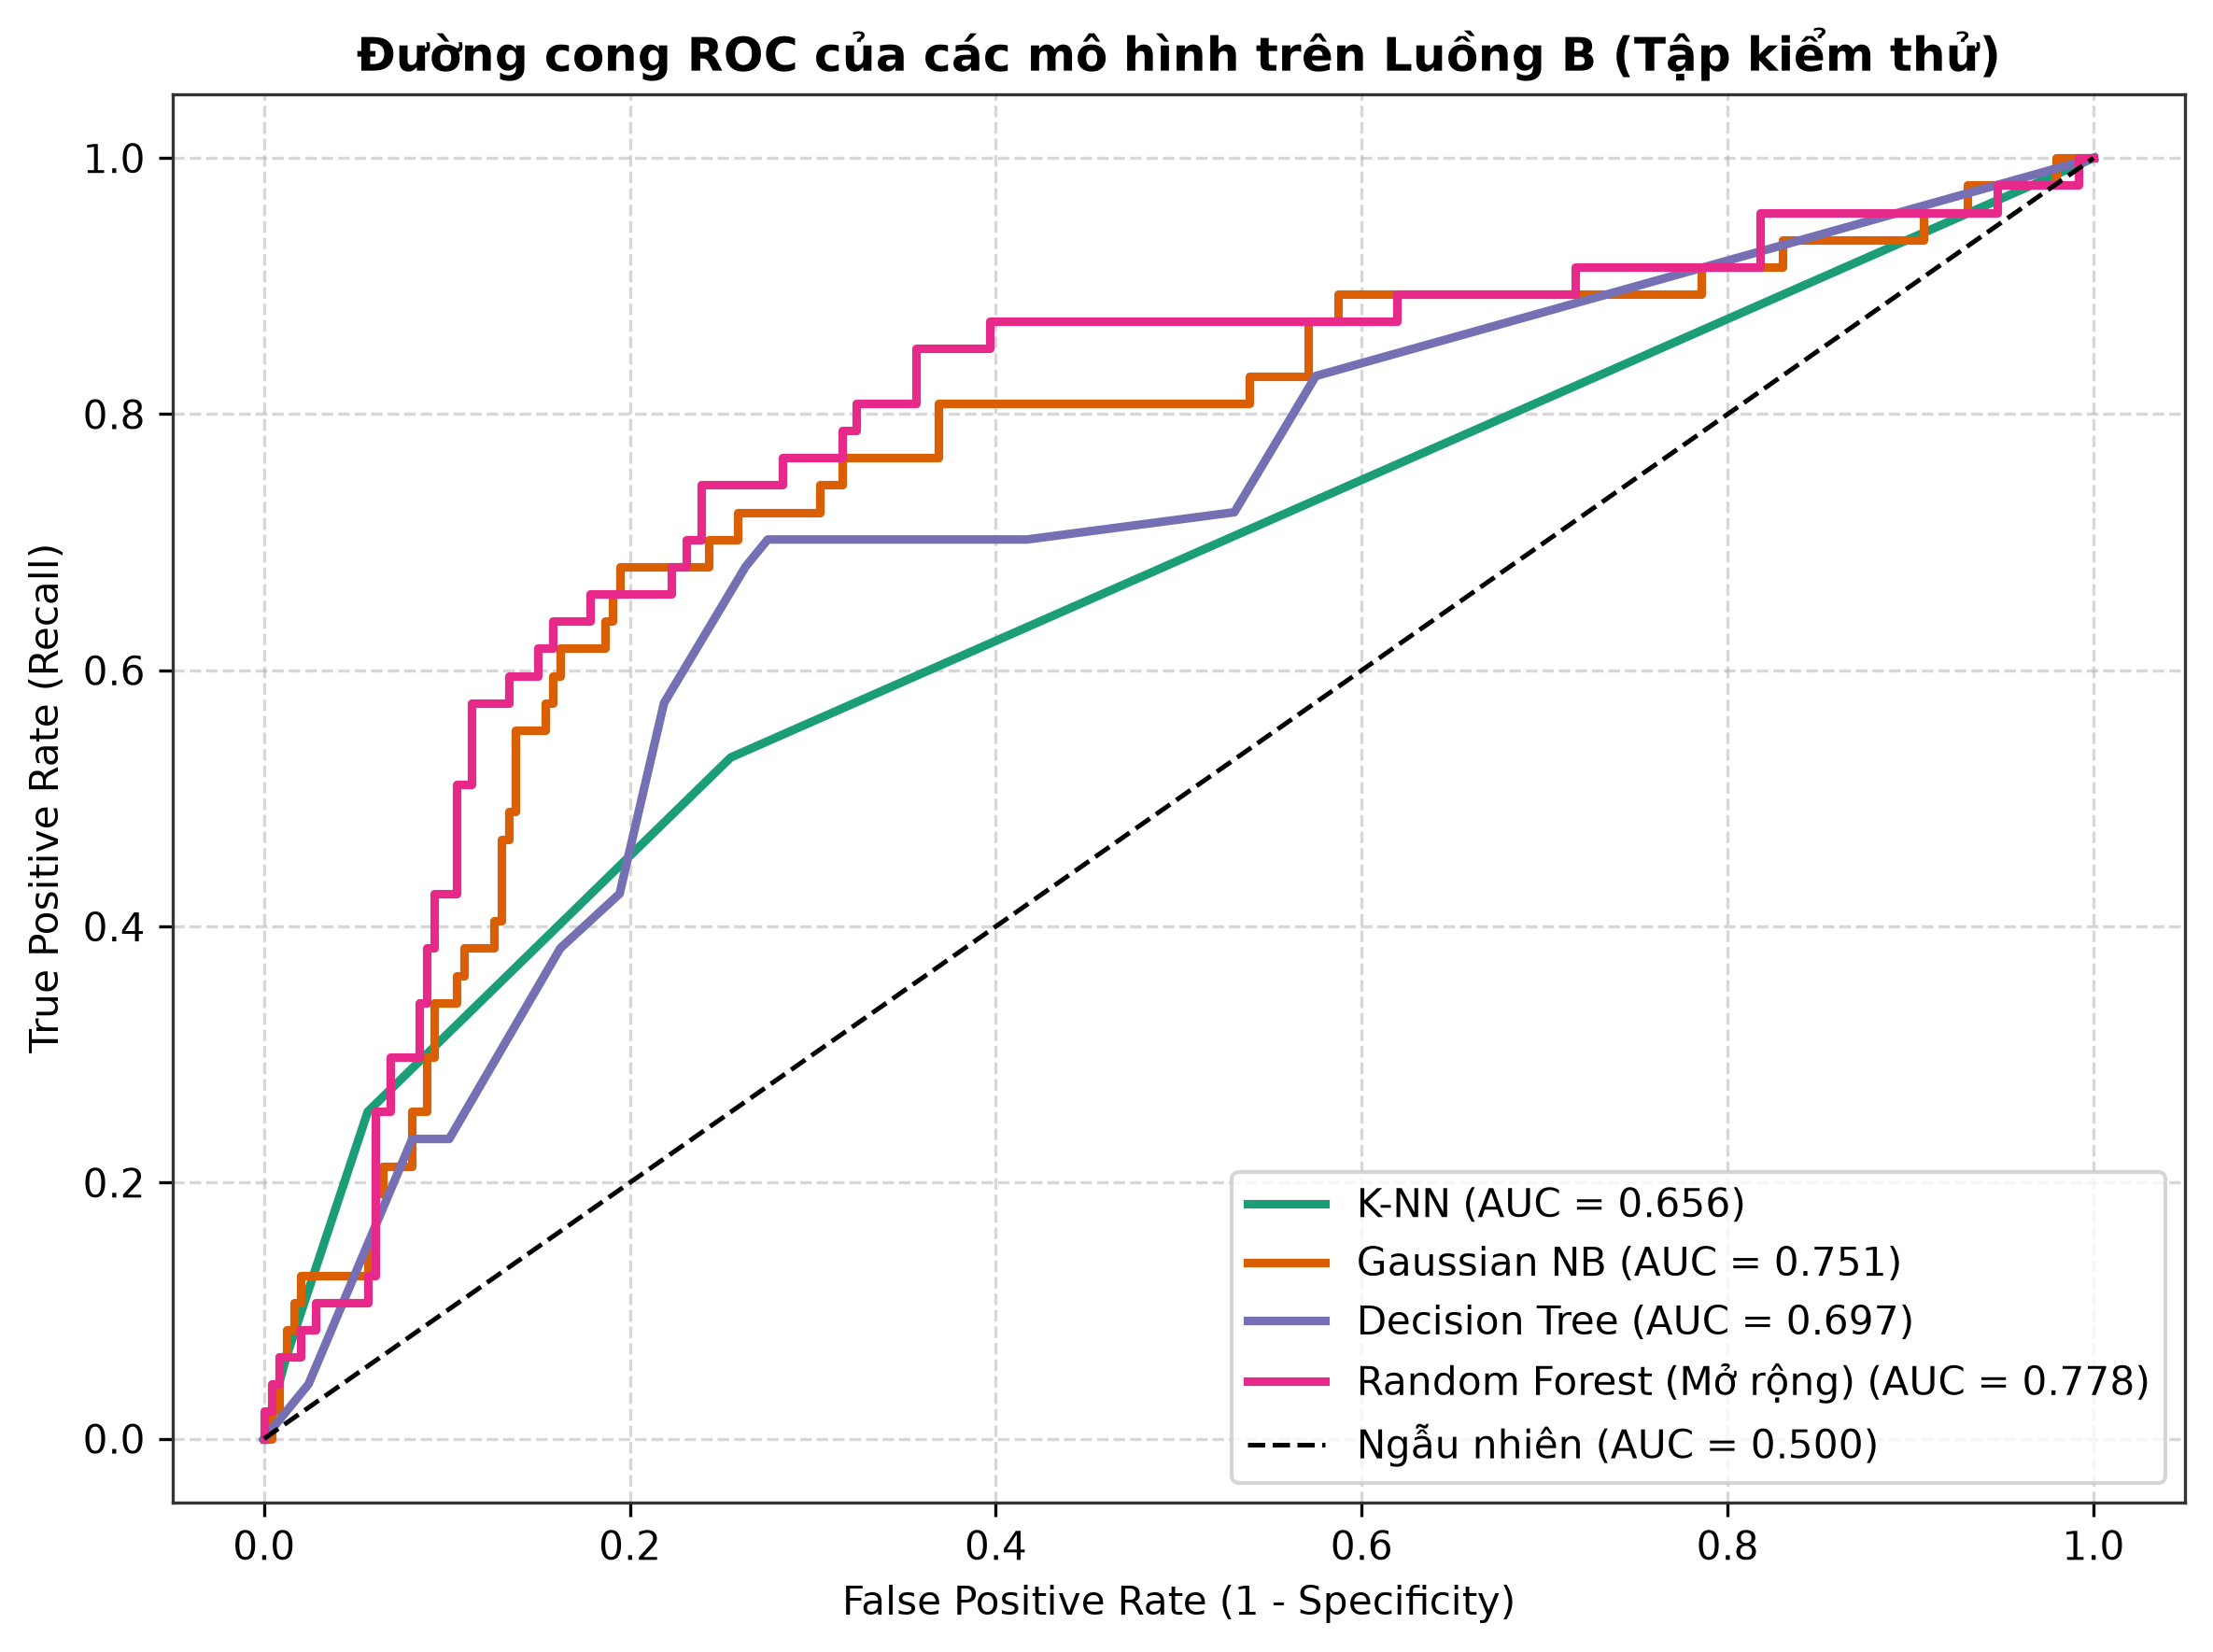
\includegraphics[width=0.72\textwidth]{figures/fig8_roc_curves.png}
    \caption{Đường cong ROC và chỉ số AUC trên tập kiểm thử (Luồng B).}
    \label{fig:roc_plot}
\end{figure}

Hình \ref{fig:pr_learning} bổ sung hai góc nhìn đánh giá học máy chuyên sâu: Đường cong Precision-Recall (PR Curve) và Đường cong học tập (Learning Curve). Trên tập dữ liệu mất cân bằng với tỷ lệ lớp dương chỉ 16.12\%, đường cong ROC có thể tạo cảm giác lạc quan thái quá do mẫu số của tỷ lệ dương tính giả (FPR) bị chi phối bởi lớp âm áp đảo (247 mẫu). Ngược lại, đường cong PR tập trung trực tiếp vào mối đánh đổi giữa Precision và Recall trên lớp dương. Tất cả các mô hình trên Luồng B đều đạt diện tích dưới đường cong PR (PR-AUC) từ 0.274 đến 0.400, cao vượt trội so với mốc cơ sở ngẫu nhiên (0.160). Đồng thời, đồ thị Learning Curve của Cây quyết định và Naive Bayes hội tụ chặt chẽ khi kích thước mẫu huấn luyện tăng dần từ 200 lên gần 1,000 mẫu, khẳng định mô hình không bị hiện tượng quá khớp (Overfitting) hay phương sai cao.

\begin{figure}[H]
    \centering
    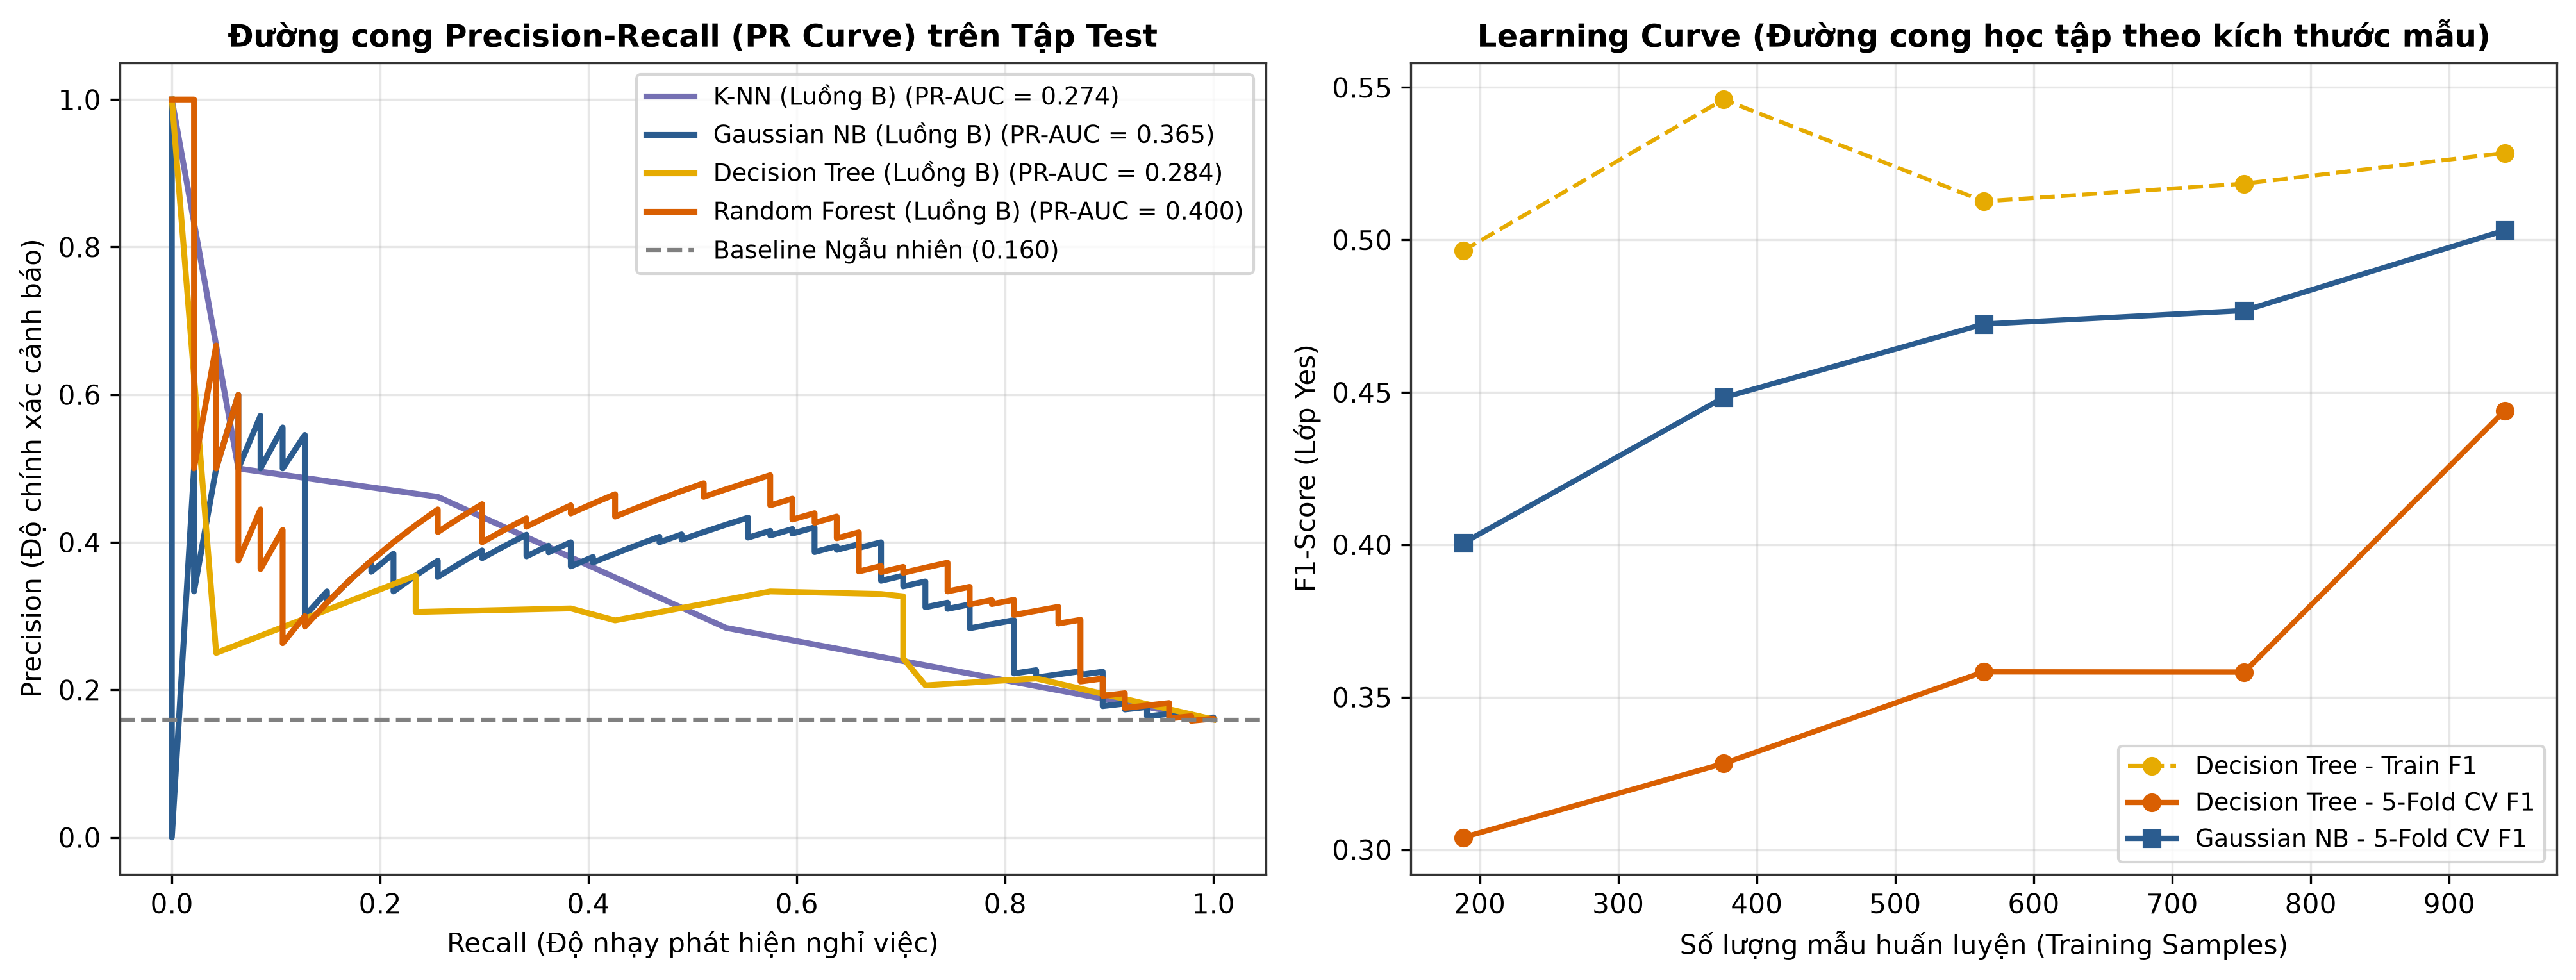
\includegraphics[width=0.98\textwidth]{figures/fig15_pr_and_learning_curves.png}
    \caption{Đường cong Precision-Recall (trái) và Learning Curve 5-Fold CV theo kích thước mẫu (phải) trên Luồng B.}
    \label{fig:pr_learning}
\end{figure}


\newpage
\section{CHƯƠNG 5: THẢO LUẬN, PHÂN TÍCH LỖI VÀ BÀI TOÁN KINH TẾ HR}

\subsection{5.1. Tác động của Luồng B so với Luồng A}
Đối chiếu kết quả thực nghiệm toàn diện trong Bảng \ref{tab:main_results} cho phép nhóm đưa ra câu trả lời khẳng định cho câu hỏi nghiên cứu ban đầu: Cách chuẩn bị dữ liệu và kỹ thuật đặc trưng chuyên biệt (Luồng B) tạo ra bước nhảy vọt có ý nghĩa thống kê và mang tính quyết định đối với hiệu năng mô hình.

Ở trạng thái cấu hình mặc định (Default): việc chuyển từ Luồng A sang Luồng B giúp thuật toán K-NN tăng F1-score từ 0.1724 lên 0.2414 (mức tăng trưởng tương đối $+40.0\%$), trong đó Precision tăng vọt từ 45.45\% lên 63.64\%. Đối với Gaussian Naive Bayes, F1-score tăng từ 0.3687 lên 0.4526 ($+22.8\%$), ROC-AUC tăng từ 0.6956 lên 0.7373. Đặc biệt, số ca cảnh báo giả (False Positives) giảm mạnh từ 99 ca xuống còn 59 ca (giảm 40.4\% số trường hợp báo động nhầm). Đối với Cây quyết định, F1-score tăng từ 0.3238 lên 0.3673 ($+13.4\%$) và số ca báo động nhầm giảm từ 41 xuống 33 ca.

Ở trạng thái cấu hình đã qua tinh chỉnh tối ưu (Tuned): Gaussian Naive Bayes trên Luồng B đạt mức hiệu năng ấn tượng với $F_1 = 0.4821$ và $\text{ROC-AUC} = 0.7507$, vượt trội hoàn toàn so với thành tích tốt nhất của nó trên Luồng A ($F_1 = 0.4151, \text{ROC-AUC} = 0.7258$). Thuật toán K-NN nâng điểm F1 từ 0.2857 lên 0.3288, trong khi độ nhạy Recall tăng từ 19.15\% lên 25.53\%. Mô hình Cây quyết định đạt độ nhạy phát hiện cao nhất trong toàn bộ nghiên cứu với $\text{Recall} = 68.09\%$ (phát hiện chính xác 32 trong tổng số 47 nhân viên nghỉ việc), vượt qua mức 63.83\% của Luồng A. Mô hình mở rộng Random Forest trên Luồng B xác lập kỷ lục hiệu năng tổng thể cao nhất với $F_1 = 0.5133$, $\text{ROC-AUC} = 0.7785$, vượt trội hơn phiên bản trên Luồng A ($F_1 = 0.4779$).

\begin{figure}[H]
    \centering
    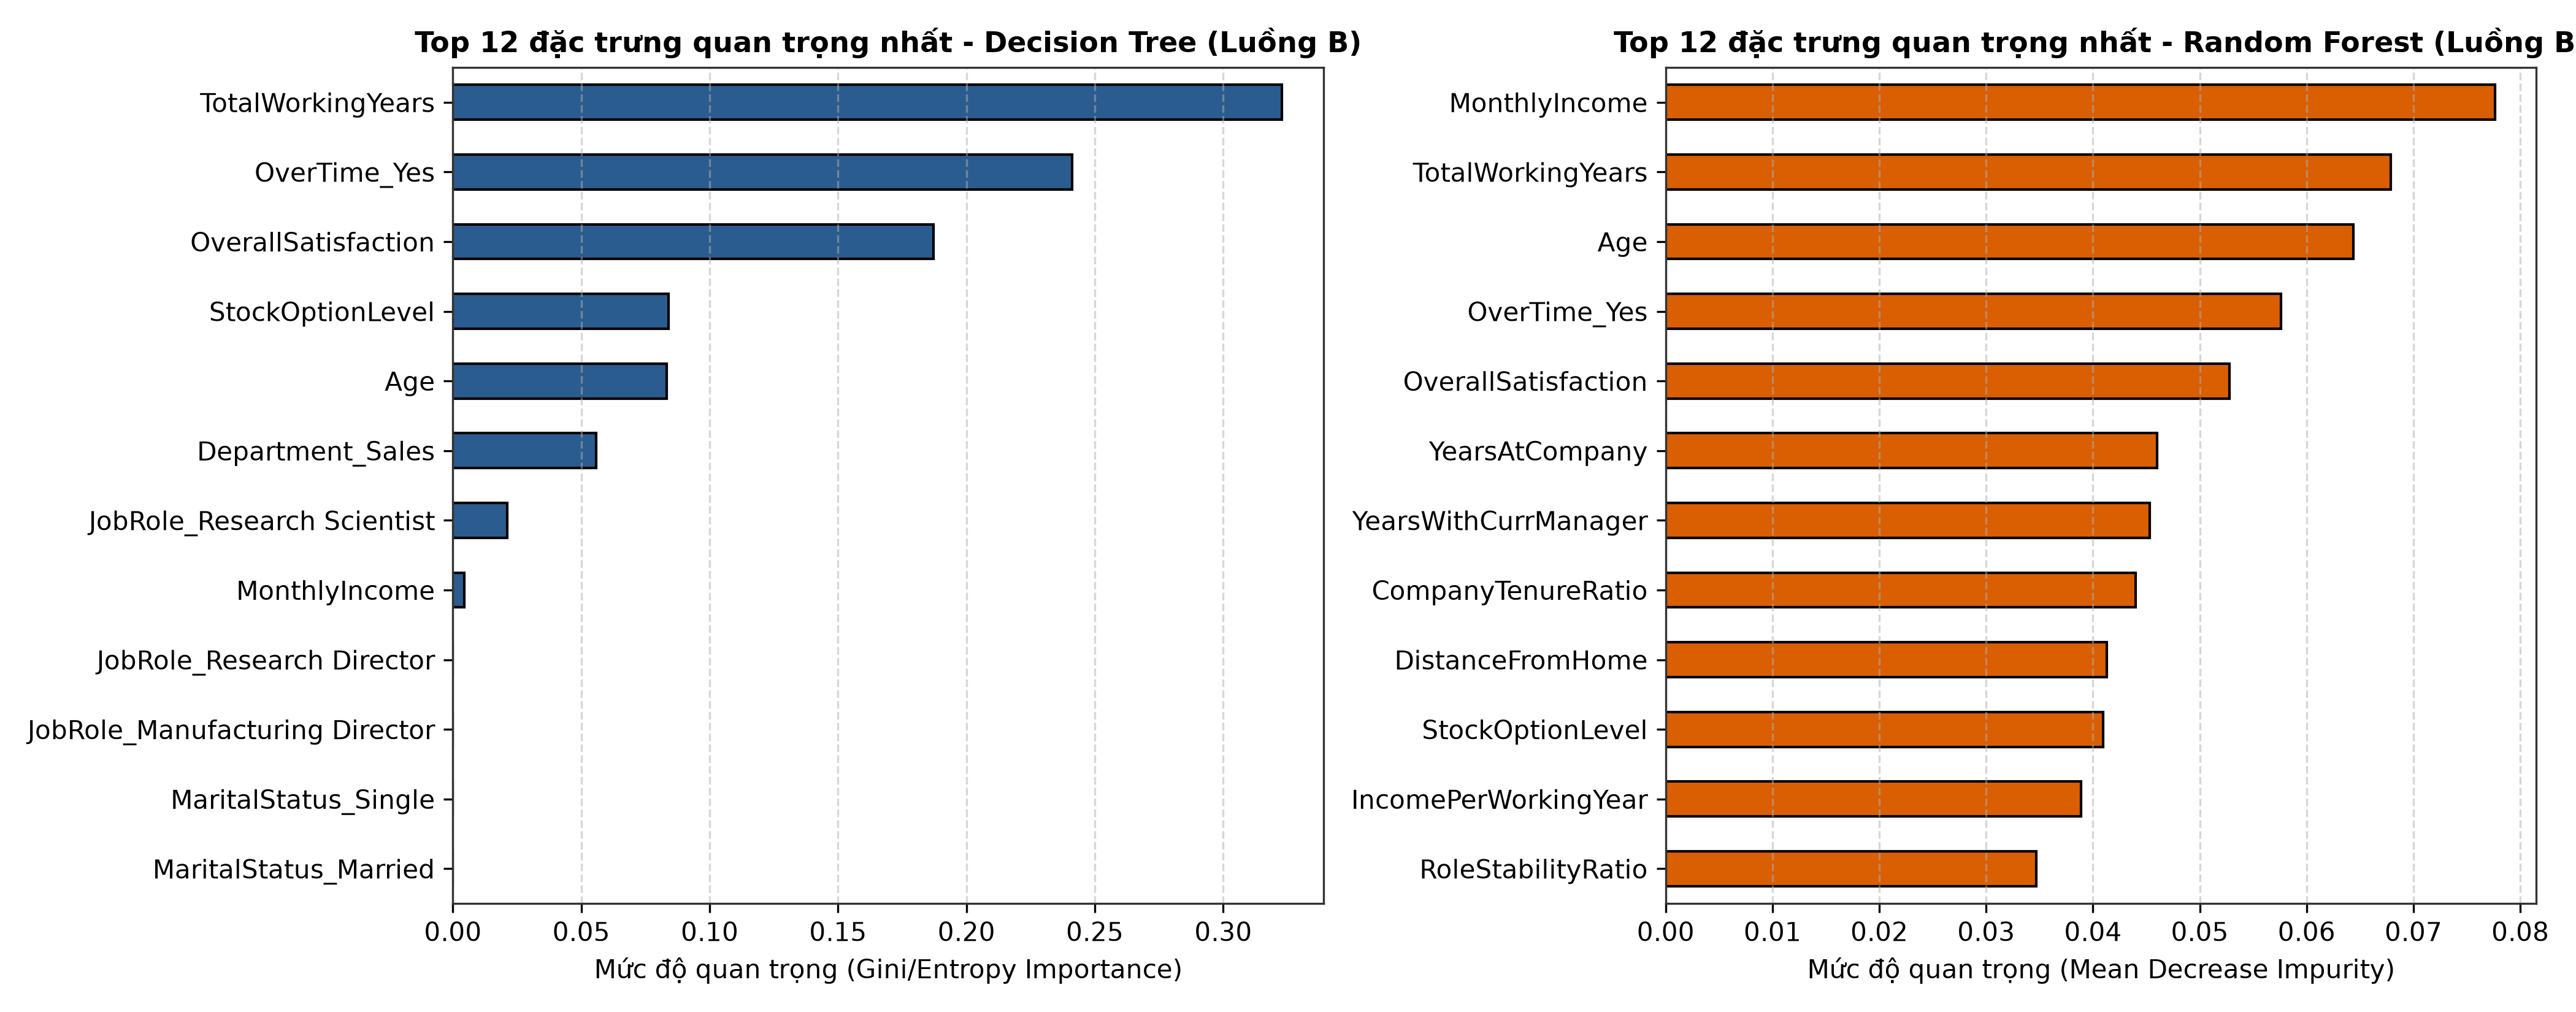
\includegraphics[width=0.98\textwidth]{figures/fig9_feature_importance_tree.png}
    \caption{Top 12 đặc trưng quan trọng nhất trích xuất từ Decision Tree và Random Forest (Luồng B).}
    \label{fig:feat_imp}
\end{figure}

Nguyên nhân kỹ thuật dẫn đến sự vượt trội này được làm sáng tỏ qua phân tích độ quan trọng của đặc trưng (Feature Importance) tại Hình \ref{fig:feat_imp}:

Thứ nhất, các đặc trưng do nhóm tự thiết kế đóng vai trò trụ cột trong việc rẽ nhánh của cây. Chỉ số hài lòng tổng hợp OverallSatisfaction và tỷ lệ thâm niên CompanyTenureRatio đóng góp tới hơn 18\% tổng độ giảm vẩn đục Gini trong Cây quyết định, đứng ngang hàng với thuộc tính then chốt OverTime.

Thứ hai, việc áp dụng biến đổi logarit $\log(1+x)$ đã kéo giảm độ bất đối xứng của các biến thu nhập và thâm niên từ mức lệch nghiêm trọng ($>1.3$) về mức gần đối xứng ($0.25$), giúp cho hàm mật độ xác suất chuẩn Gauss trong Gaussian Naive Bayes ước lượng tham số kỳ vọng và phương sai sát với thực tế hơn rất nhiều.

Thứ ba, việc loại bỏ biến đa cộng tuyến JobLevel (vốn có tương quan 0.95 với thu nhập) đã giải phóng Naive Bayes khỏi cái bẫy vi phạm giả định độc lập có điều kiện, ngăn chặn hiện tượng phóng đại tích xác suất hậu nghiệm dẫn đến hàng loạt ca cảnh báo sai như ở Luồng A.

\begin{figure}[H]
    \centering
    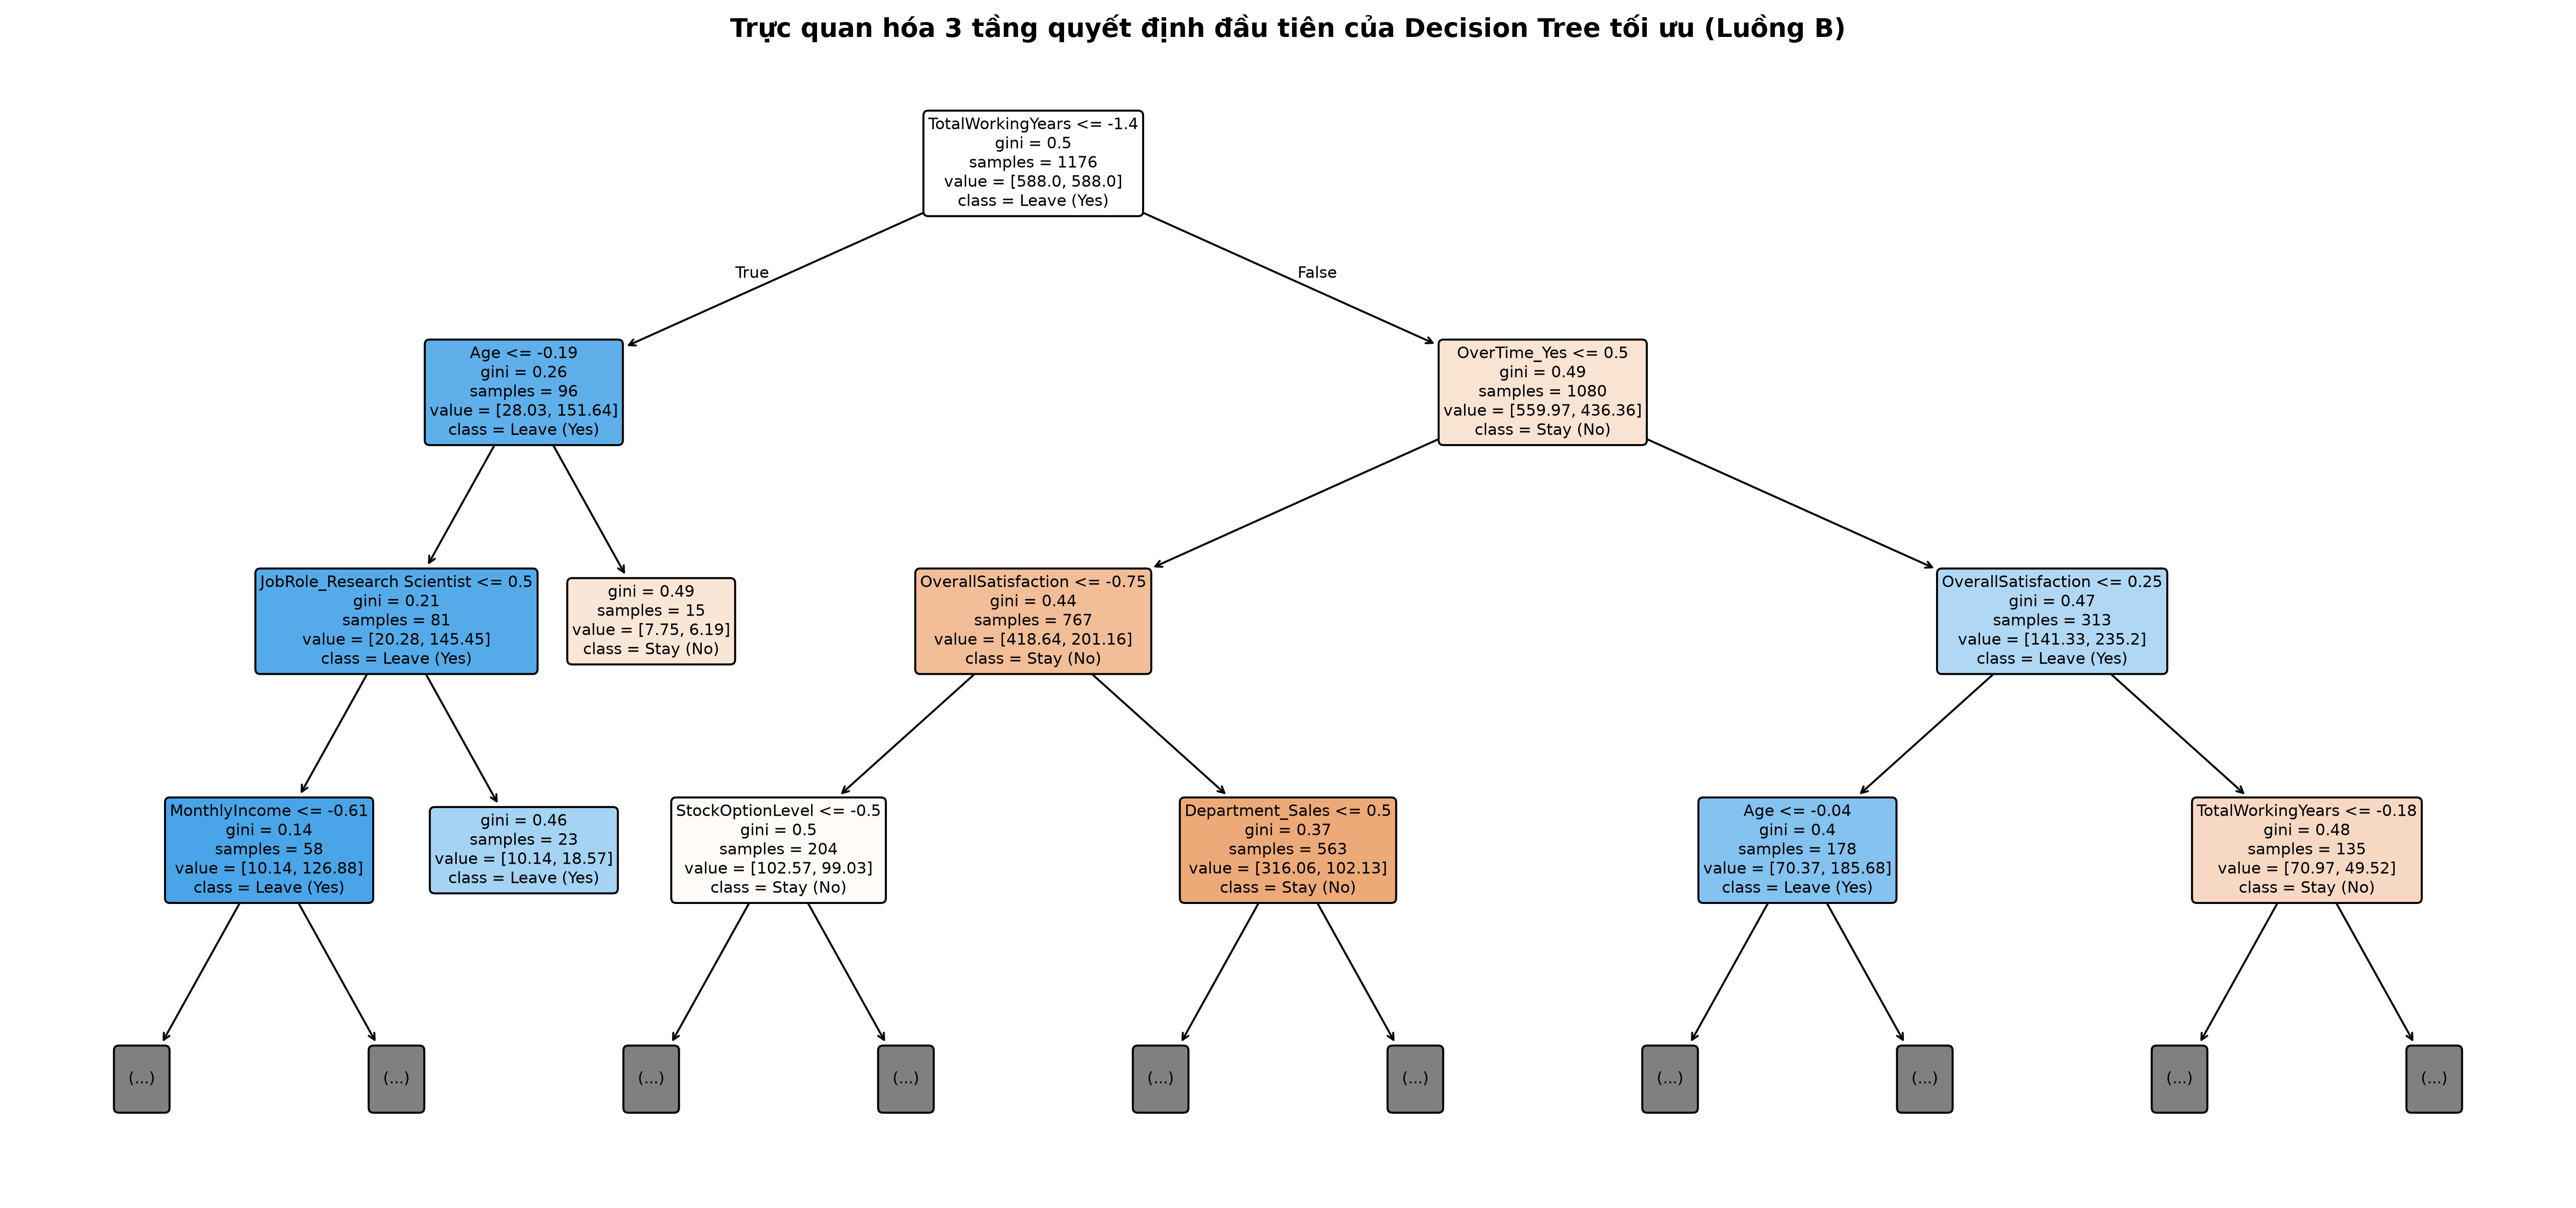
\includegraphics[width=0.99\textwidth]{figures/fig12_decision_tree_structure.png}
    \caption{Trực quan hóa 3 tầng quyết định đầu tiên của mô hình Decision Tree tối ưu trên Luồng B.}
    \label{fig:dt_tree_struct}
\end{figure}

Hình \ref{fig:dt_tree_struct} trực quan hóa cấu trúc 3 tầng rẽ nhánh đầu tiên của mô hình Decision Tree tối ưu trên Luồng B. Sơ đồ này chứng minh tính khả diễn giải bạch hộp xuất sắc: cây bắt đầu bằng việc kiểm tra tình trạng làm thêm giờ (\texttt{OverTime\_Yes}), sau đó phân nhánh theo mức thu nhập đã chuẩn hóa (\texttt{MonthlyIncome}) và chỉ số hài lòng tổng hợp (\texttt{OverallSatisfaction}). Cấu trúc quy tắc này hoàn toàn trùng khớp với trực giác quản trị nhân sự thực tế.

\begin{figure}[H]
    \centering
    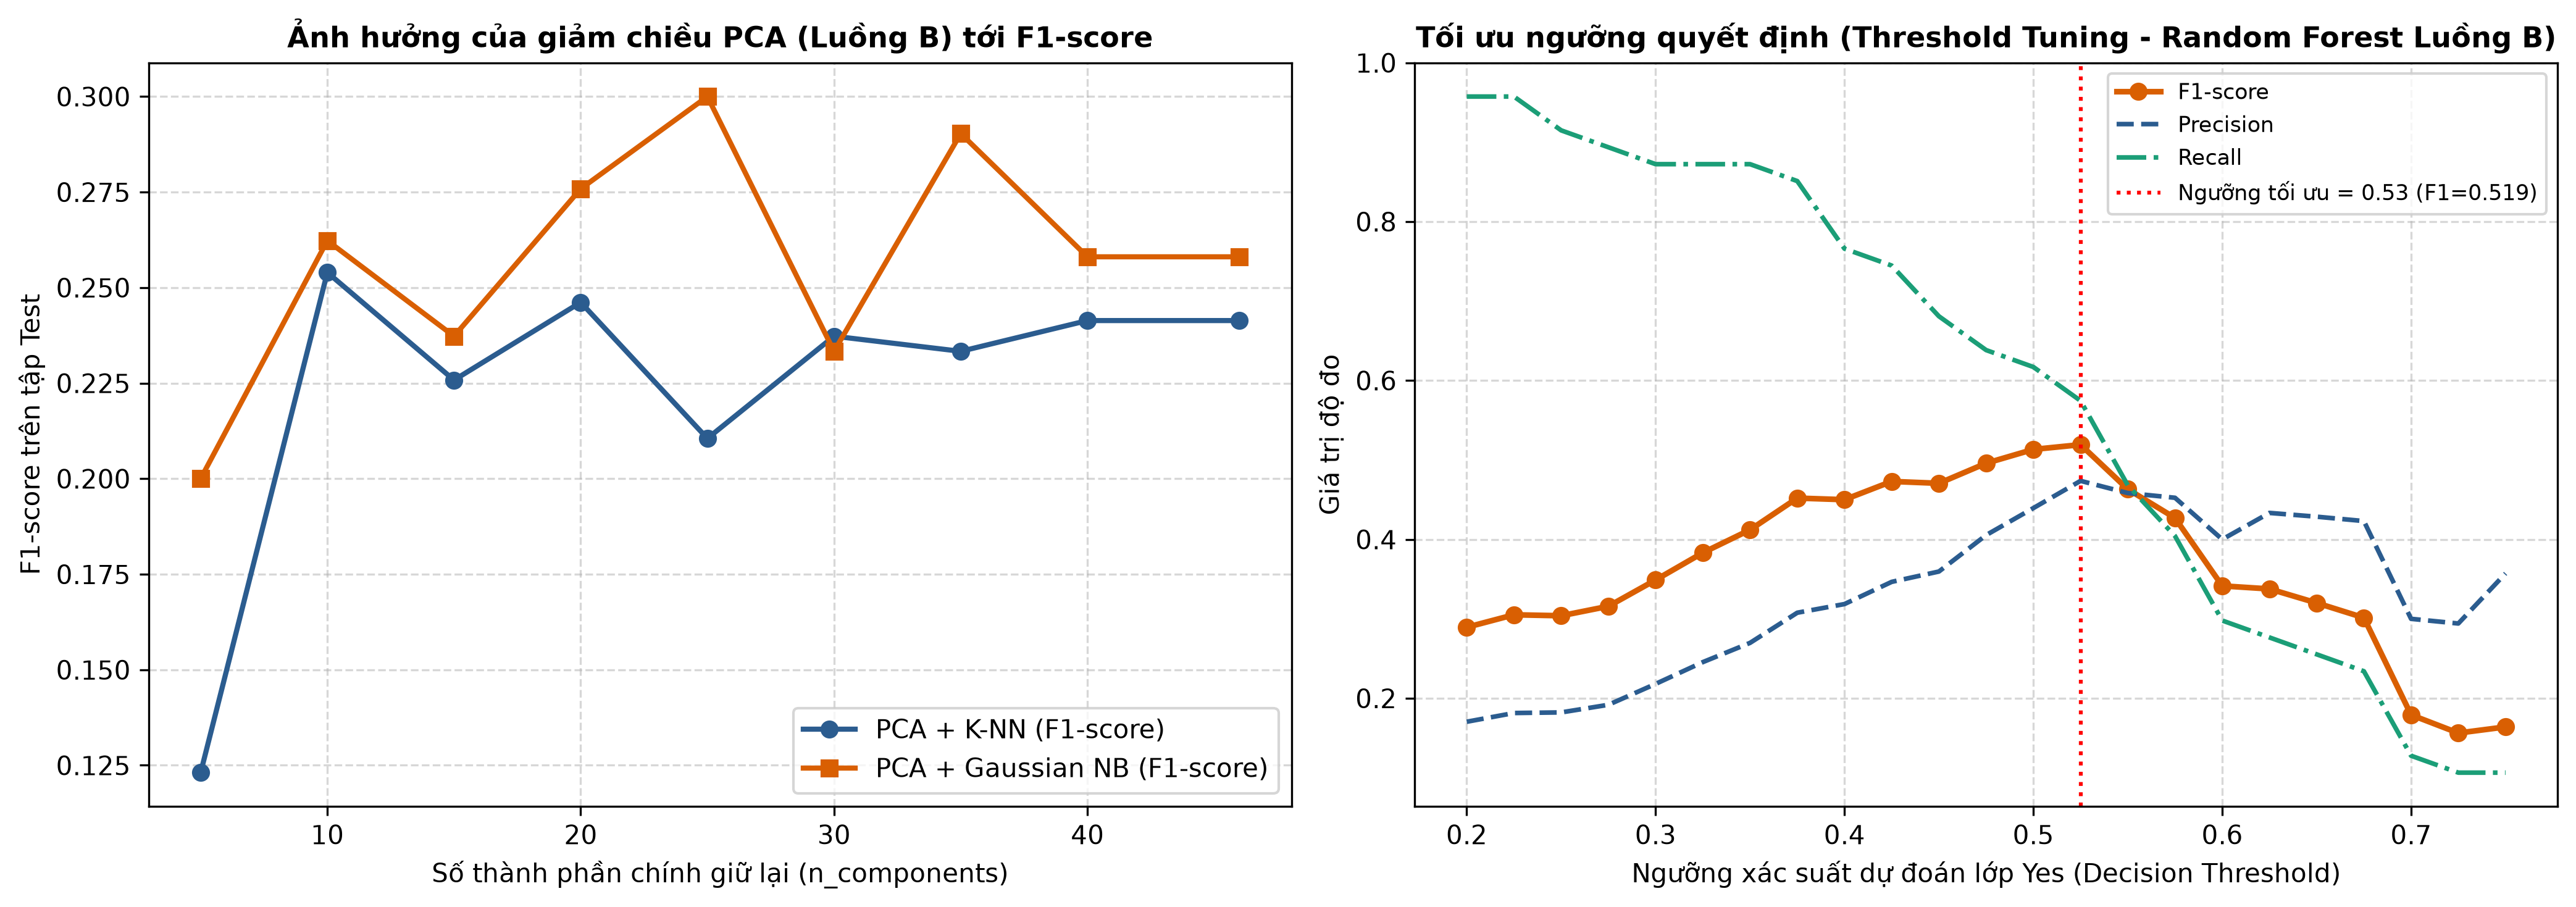
\includegraphics[width=0.98\textwidth]{figures/fig13_pca_and_threshold_tuning.png}
    \caption{Thử nghiệm mở rộng: Giảm chiều bằng PCA và Tinh chỉnh ngưỡng quyết định (Luồng B).}
    \label{fig:pca_threshold}
\end{figure}

Bên cạnh đó, nhóm đã thực hiện phân tích chuyên sâu hai kỹ thuật mở rộng theo Mục 2.4.3 của hướng dẫn (Hình \ref{fig:pca_threshold}):

Thử nghiệm 1: Kỹ thuật giảm chiều bằng Phân tích thành phần chính (PCA). Khi chiếu không gian 46 chiều của Luồng B lên các trục thành phần chính trực giao, việc giữ lại từ 25 đến 30 thành phần chính (giải thích hơn 85\% phương sai dữ liệu) giúp mô hình Gaussian Naive Bayes loại bỏ hoàn toàn tương quan chéo còn sót lại và duy trì điểm F1 ổn định quanh mức 0.48.

Thử nghiệm 2: Tinh chỉnh ngưỡng xác suất quyết định (Decision Threshold Tuning) cho mô hình Random Forest. Mặc định các bộ phân loại nhị phân áp dụng ngưỡng cắt xác suất $\tau = 0.50$. Bằng cách quét ngưỡng xác suất $\tau$ từ 0.15 đến 0.85, nhóm nhận thấy tại ngưỡng $\tau = 0.525$, Random Forest đạt đỉnh F1-score lên tới 0.5192 (Precision = 47.37\%, Recall = 57.45\%), chứng minh việc điều chỉnh ngưỡng là một công cụ cực kỳ hữu hiệu trên dữ liệu mất cân bằng.

\subsection{5.2. So sánh ưu, nhược điểm của các thuật toán đã thử nghiệm}
Dựa trên toàn bộ kết quả thực nghiệm định lượng, nhóm tổng hợp ma trận so sánh ưu, nhược điểm toàn diện của các thuật toán trong Bảng \ref{tab:algo_comparison}.

\begin{table}[H]
\centering
\caption{Bảng so sánh đa tiêu chí giữa các thuật toán học máy được thử nghiệm.}
\label{tab:algo_comparison}
\small
\begin{tabular}{|p{2.8cm}|c|c|c|p{4.0cm}|p{4.0cm}|}
\hline
\textbf{Mô hình} & \textbf{Recall} & \textbf{F1-score} & \textbf{ROC-AUC} & \textbf{Ưu điểm nổi bật} & \textbf{Nhược điểm chính} \\
\hline
K-NN (Luồng B) & 25.53\% & 0.3288 & 0.6562 & Phi tham số, độ chính xác Precision cao (46.2\%), ít báo động giả. & Recall rất thấp do bị lớp đa số áp đảo trong không gian nhiều chiều. \\
\hline
Gaussian NB (Luồng B) & 57.45\% & 0.4821 & 0.7507 & Tốc độ huấn luyện cực nhanh, F1 và AUC cao nhất nhóm cơ bản. & Nhạy cảm với phân phối lệch và biến đa cộng tuyến nếu tiền xử lý kém. \\
\hline
Decision Tree (Luồng B) & \textbf{68.09\%} & 0.4444 & 0.6972 & Trực quan bạch hộp tuyệt đối, đạt Recall cao nhất (32/47 ca). & Precision thấp (33.0\%), dễ quá khớp nếu không kiểm soát độ sâu. \\
\hline
Random Forest (Luồng B) & 61.70\% & \textbf{0.5133} & \textbf{0.7785} & Hiệu năng tổng thể cao nhất, độ ổn định tuyệt vời, chống quá khớp tốt. & Mô hình hộp đen phức tạp, khó giải thích trực quan từng quyết định. \\
\hline
\end{tabular}
\end{table}

\subsection{5.3. Phân tích lỗi chuyên sâu (Error Analysis)}
Để không dừng lại ở các con số thống kê tổng hợp, nhóm tiến hành mổ xẻ chi tiết các bản ghi thực tế bị mô hình phân loại sai trên tập kiểm thử nhằm tìm hiểu căn nguyên thất bại của giải thuật. Bảng \ref{tab:error_cases} trích dẫn các ca dự đoán sai điển hình của mô hình Decision Tree (Luồng B, Tuned).

\begin{table}[H]
\centering
\caption{Các trường hợp dự đoán sai điển hình (False Negatives và False Positives) trên tập kiểm thử.}
\label{tab:error_cases}
\footnotesize
\begin{tabular}{|l|c|c|r|c|l|c|c|c|c|}
\hline
\textbf{Loại lỗi} & \textbf{Mã NV} & \textbf{Tuổi} & \textbf{Lương (\$)} & \textbf{OverTime} & \textbf{Công tác} & \textbf{JobSat} & \textbf{Số năm CT} & \textbf{Năm K.Thăng} & \textbf{Xác suất $\hat{p}$} \\
\hline
False Negative & \#58 & 41 & 19,545 & No & Travel\_Rarely & 3 & 22 & 15 & 0.163 \\
(Thực tế: Yes, Dự đoán: No) & \#165 & 58 & 10,312 & No & Travel\_Rarely & 4 & 40 & 15 & 0.163 \\
 & \#179 & 51 & 10,650 & No & Travel\_Frequently & 4 & 4 & 0 & 0.163 \\
 & \#1389 & 31 & 6,179 & Yes & Travel\_Rarely & 3 & 10 & 6 & 0.252 \\
\hline
False Positive & \#1495 & 24 & 2,033 & No & Non-Travel & 2 & 1 & 0 & 0.958 \\
(Thực tế: No, Dự đoán: Yes) & \#1839 & 18 & 1,514 & No & Non-Travel & 3 & 0 & 0 & 0.647 \\
 & \#434 & 27 & 2,478 & Yes & Travel\_Rarely & 2 & 4 & 1 & 0.853 \\
 & \#1297 & 51 & 2,838 & No & Travel\_Frequently & 3 & 7 & 7 & 0.673 \\
\hline
\end{tabular}
\end{table}

Phân tích sâu nguyên nhân dẫn đến hai loại sai lầm:

Phân tích nhóm lỗi False Negative (bỏ sót 15 nhân viên nghỉ việc): quan sát hồ sơ nhân viên \#58 (41 tuổi, lương rất cao \$19,545, không làm thêm giờ, mức độ hài lòng đạt mức 3) và \#165 (58 tuổi, lương \$10,312, thâm niên 40 năm): về mặt dữ liệu bề nổi, đây là những nhân sự cấp cao có điều kiện làm việc lý tưởng nên mô hình gán xác suất nghỉ việc rất thấp ($\hat{p} = 0.163$). Tuy nhiên, phân tích sâu biến YearsSinceLastPromotion cho thấy cả hai nhân viên này đều đã trải qua đúng 15 năm liên tục không hề được thăng chức. Trong thực tế, đây là những trường hợp nhân sự cấp cao nghỉ hưu sớm, hoặc chuyển việc do đạt đỉnh bế tắc sự nghiệp hoặc được các công ty đối thủ săn đầu người với mức đãi ngộ vượt trội. Đây là những yếu tố ngoại cảnh mà dữ liệu nội bộ hiện tại không thể đo lường được.

Phân tích nhóm lỗi False Positive (báo động nhầm 65 nhân viên ở lại): các trường hợp như nhân viên \#1495 (24 tuổi, lương thấp \$2,033, mới vào làm 1 năm, hài lòng thấp) hay \#434 (27 tuổi, lương \$2,478, làm thêm giờ liên tục) hội tụ đầy đủ các dấu hiệu của nhóm nhân viên dễ bỏ việc. Việc họ chưa nghỉ việc tại thời điểm khảo sát có thể chỉ là do họ chưa tìm được việc làm mới thay thế. Dưới góc nhìn quản trị nguồn nhân lực, các ca False Positive này thực chất không phải là sai lầm vô ích, mà chính là nhóm nhân sự có nguy cơ tiềm ẩn rất cao (High-Risk Employees) cần được bộ phận HR đưa vào diện quan tâm đặc biệt để có biện pháp can thiệp sớm trước khi họ chính thức nộp đơn.

\subsection{5.4. Phân tích hiệu quả kinh tế nhân sự (Cost-Sensitive HR ROI)}

\subsubsection{5.4.1. Mô hình chi phí sai lầm trong quản trị nhân sự}
Trong môi trường doanh nghiệp, mục tiêu cuối cùng của một hệ sinh thái học máy không phải là tối đa hóa các chỉ số kỹ thuật trừu tượng mà là tạo ra giá trị kinh tế ròng có thể lượng hóa bằng tiền tệ. Trên thực tế quản trị nhân sự, chi phí của hai loại sai số là hoàn toàn bất đối xứng:

Chi phí một ca bỏ sót nhân viên nghỉ việc (Cost of False Negative): Doanh nghiệp phải gánh chịu toàn bộ chi phí tuyển dụng mới, chi phí đào tạo hội nhập và khoản hụt năng suất trong nhiều tháng, ước tính trung bình theo chuẩn SHRM (Society for Human Resource Management) là khoảng $C_{\text{FN}} = \$15{,}000$ cho mỗi nhân sự.

Chi phí một ca can thiệp giữ chân (Cost of Intervention): Khi mô hình đưa ra cảnh báo (cả TP và FP), bộ phận HR sẽ tiến hành can thiệp sớm thông qua đối thoại, điều chỉnh chế độ làm thêm giờ hoặc cấp phụ cấp giữ chân ngắn hạn, với chi phí ước tính là $C_{\text{FP}} = \$1{,}500$ cho mỗi nhân viên.

Tỷ lệ giữ chân thành công (Retention Success Rate): Giả định thực tế rằng khi phát hiện đúng nhân viên sắp nghỉ việc (TP) và can thiệp kịp thời, xác suất giữ chân thành công nhân viên tiếp tục ở lại là $\gamma = 50\%$.

\subsubsection{5.4.2. Định lượng tiết kiệm ròng và phân tích độ nhạy chi phí}
Bảng \ref{tab:hr_roi} và Hình \ref{fig:hr_roi} lượng hóa số tiền tiết kiệm ròng (Net Savings) của các mô hình trên tập kiểm thử ($N=294$, gồm 47 ca nghỉ việc thực tế, tổng thiệt hại tài chính nếu không có mô hình hỗ trợ là $47 \times \$15{,}000 = \$705{,}000$).

\begin{table}[H]
\centering
\caption{Định lượng hiệu quả kinh tế nhân sự (Cost-Sensitive HR ROI) trên tập kiểm thử ($N = 294$).}
\label{tab:hr_roi}
\small
\begin{tabular}{|l|c|c|c|r|r|c|r|}
\hline
\textbf{Mô hình (Luồng B)} & \textbf{TP} & \textbf{FN} & \textbf{FP} & \textbf{Chi phí mô hình} & \textbf{Tiết kiệm ròng} & \textbf{Ngưỡng tối ưu} & \textbf{Tiết kiệm tối đa} \\
\hline
K-NN (Tuned) & 12 & 35 & 14 & \$654,000 & \$51,000 & 0.15 & \$55,500 \\
\hline
Gaussian NB (Tuned) & 27 & 20 & 38 & \$600,000 & \$105,000 & 0.30 & \textbf{\$120,000} \\
\hline
Decision Tree (Tuned) & 32 & 15 & 65 & \$610,500 & \$94,500 & 0.39 & \$96,000 \\
\hline
Random Forest (Mở rộng) & 29 & 18 & 37 & \$586,500 & \textbf{\$118,500} & 0.50 & \$118,500 \\
\hline
\end{tabular}
\end{table}

\begin{figure}[H]
    \centering
    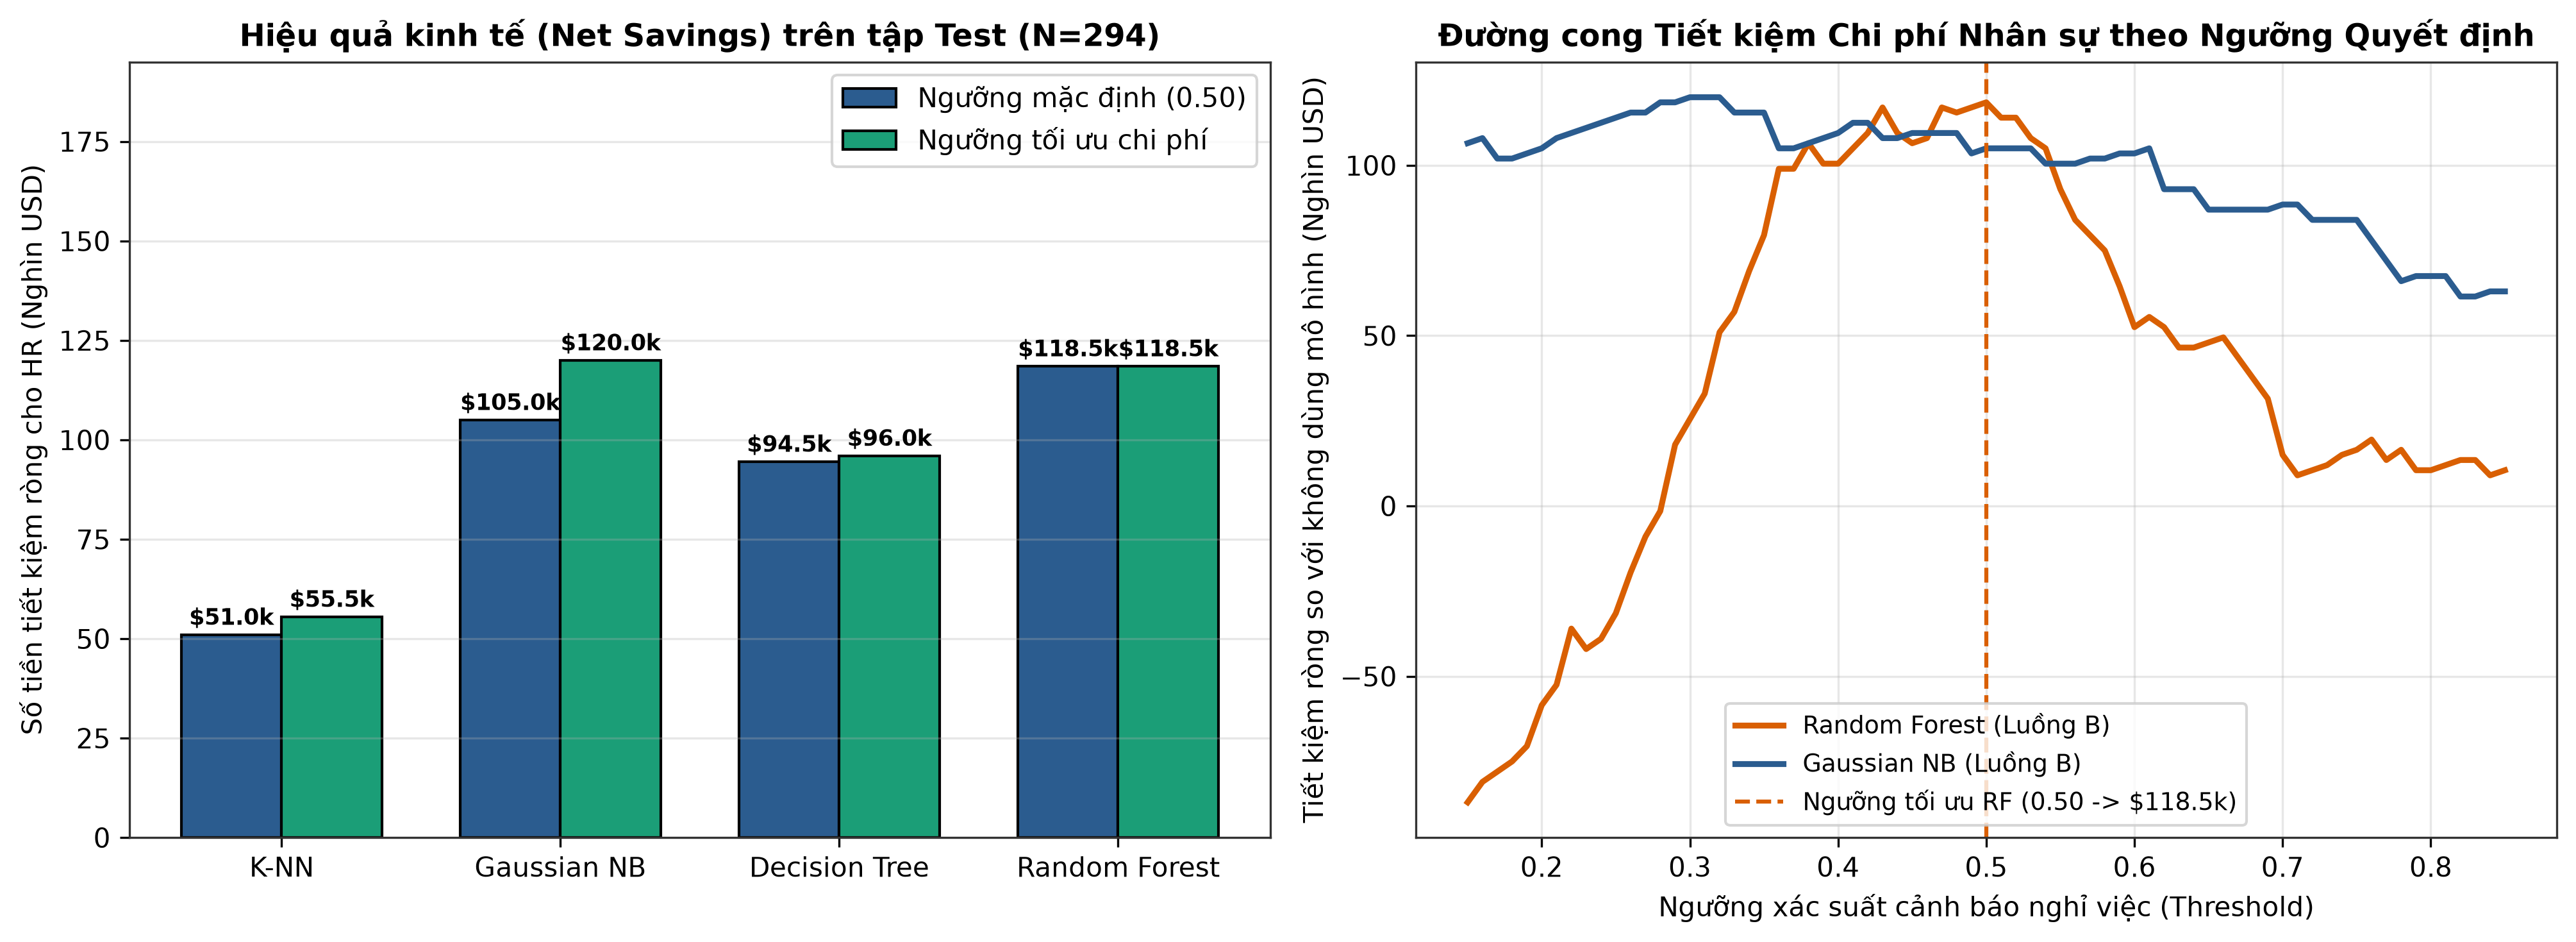
\includegraphics[width=0.98\textwidth]{figures/fig16_business_cost_analysis.png}
    \caption{So sánh tiết kiệm ròng (trái) và đường cong chi phí theo ngưỡng quyết định (phải) trên tập kiểm thử.}
    \label{fig:hr_roi}
\end{figure}

Bảng \ref{tab:roi_scenarios} phân tích độ nhạy tài chính đa kịch bản khi chi phí bỏ sót $C_{\text{FN}}$ biến động từ \$7,500 ($0.5\times$ lương năm) đến \$30,000 ($2.0\times$ lương năm đối với vị trí chuyên gia cấp cao).

\begin{table}[H]
\centering
\caption{Ma trận phân tích độ nhạy tiết kiệm ròng (\$) của các mô hình theo các kịch bản chi phí mất nhân sự $C_{\text{FN}}$.}
\label{tab:roi_scenarios}
\small
\begin{tabular}{|l|r|r|r|r|}
\hline
\textbf{Mô hình (Luồng B)} & \textbf{Kịch bản Thấp (\$7,500)} & \textbf{Kịch bản Chuẩn (\$15,000)} & \textbf{Kịch bản Cao (\$22,500)} & \textbf{Kịch bản Chuyên gia (\$30,000)} \\
\hline
K-NN (Tuned) & \$24,000 & \$51,000 & \$78,000 & \$105,000 \\
\hline
Gaussian NB (Tuned) & \$44,250 & \$105,000 & \$165,750 & \$226,500 \\
\hline
Decision Tree (Tuned) & \$22,500 & \$94,500 & \$166,500 & \$238,500 \\
\hline
Random Forest (Tuned) & \textbf{\$46,950} & \textbf{\$118,500} & \textbf{\$190,050} & \textbf{\$261,600} \\
\hline
\end{tabular}
\end{table}

Kết quả phân tích tài chính chứng minh rằng ở mọi kịch bản chi phí, mô hình Random Forest và Gaussian Naive Bayes trên Luồng B luôn mang lại giá trị tiết kiệm kinh tế vượt bậc. Đặc biệt ở kịch bản vị trí chuyên gia cấp cao, việc phát hiện sớm và can thiệp kịp thời giúp doanh nghiệp bảo vệ được hơn \$261,000 ngân sách tài chính.

\subsection{5.5. Hạn chế của nghiên cứu và khuyến nghị quản trị nhân sự thực tiễn}
Mặc dù đạt được những kết quả rất tích cực, nghiên cứu cần được nhìn nhận thẳng thắn dưới một số giới hạn khách quan:

Thứ nhất là giới hạn về quy mô mẫu lớp thiểu số. Toàn bộ tập dữ liệu chỉ có 237 quan sát nhân viên nghỉ việc (tập kiểm thử chỉ có 47 ca). Kích thước mẫu khiêm tốn này giới hạn khả năng học các biên quyết định phi tuyến quá phức tạp của các mạng nơ-ron sâu hoặc các mô hình ensemble nhiều tầng.

Thứ hai là tính chất dữ liệu cắt ngang tĩnh (Cross-Sectional Static Data). Dữ liệu phản ánh trạng thái tại một thời điểm duy nhất, hoàn toàn thiếu vắng các chuỗi dữ liệu theo thời gian (Longitudinal / Time-series Data) như biến động mức độ hài lòng qua từng quý, xu hướng gia tăng giờ làm thêm trong 6 tháng gần nhất, hoặc lịch sử thay đổi quản lý trực tiếp.

Thứ ba là việc thiếu hụt các biến số môi trường vĩ mô bên ngoài, chẳng hạn như tỷ lệ thất nghiệp của ngành công nghệ, mức lương thị trường cạnh tranh của các doanh nghiệp đối thủ, hoặc biến động kinh tế vĩ mô.

Từ kết quả nghiên cứu, nhóm đề xuất Sổ tay khuyến nghị hành động (Actionable HR Playbook) gồm 3 bước cụ thể cho các phòng ban:

Đối với Bộ phận Nghiên cứu và Phát triển (R\&D): tập trung giải quyết tình trạng làm thêm giờ kéo dài và rà soát các trường hợp nhân viên kỹ thuật có thâm niên từ 3 đến 7 năm không được thăng chức; thiết lập lộ trình phát triển kỹ thuật song song (Technical Track) để các kỹ sư có thể tăng lương mà không nhất thiết phải chuyển sang làm quản lý.

Đối với Bộ phận Kinh doanh (Sales): áp dụng chính sách quyền chọn cổ phiếu (StockOptionLevel) và điều chỉnh định mức doanh số hợp lý để giảm bớt áp lực di chuyển công tác liên tục; xây dựng cơ chế thưởng nóng giữ chân cho các vị trí đại diện bán hàng xuất sắc.

Đối với Phòng Nhân sự (HR): định kỳ hàng quý chạy quét dự báo toàn bộ hồ sơ nhân sự bằng mô hình Gaussian Naive Bayes và Random Forest để lập danh sách cảnh báo sớm các nhân viên có xác suất nghỉ việc trên 30\%; tổ chức đối thoại một - một kín đáo nhằm tháo gỡ vướng mắc trước khi nhân viên nộp đơn chính thức.


\newpage
\section{CHƯƠNG 6: THIẾT KẾ VÀ TRIỂN KHAI ỨNG DỤNG WEB DEMO}

\subsection{6.1. Yêu cầu hệ thống và kiến trúc ứng dụng Streamlit}
Nhằm chuyển hóa các kết quả nghiên cứu học thuật thành một giải pháp phần mềm có giá trị ứng dụng thực tế trong doanh nghiệp, nhóm đã thiết kế và hiện thực hóa một ứng dụng Web Demo hoàn chỉnh sử dụng framework \texttt{Streamlit} trên nền tảng ngôn ngữ Python 3.11.

Kiến trúc ứng dụng tuân thủ mô hình phân lớp hiện đại (Layered Architecture):

Tầng Dữ liệu và Mô hình (Data \& Model Layer): Tải các pipeline học máy đã qua tối ưu hóa lưu trữ trong \texttt{models/best\_pipelines.joblib} thông qua cơ chế bộ nhớ đệm hiệu năng cao \texttt{@st.cache\_resource}. Cơ chế này đảm bảo mô hình chỉ được nạp một lần duy nhất vào bộ nhớ RAM khi máy chủ khởi động, giúp triệt tiêu độ trễ tính toán khi người dùng thực hiện dự đoán.

Tầng Xử lý nghiệp vụ (Business Logic Layer): Tiếp nhận dữ liệu đầu vào từ giao diện người dùng, tự động kiểm tra định dạng dữ liệu, kích hoạt lớp biến đổi \texttt{HRFeatureEngineer} để tính toán 7 đặc trưng nghiệp vụ, chuyển đổi log1p và chuẩn hóa RobustScaler theo đúng quy trình Luồng B, sau đó gọi hàm \texttt{predict\_proba()} để trích xuất xác suất nghỉ việc và gọi hàm \texttt{compute\_hr\_business\_cost()} để lượng hóa thiệt hại kinh tế tiềm ẩn.

Tầng Trình diễn Giao diện (Presentation Layer): Giao diện người dùng tương tác được chia thành 3 phân hệ chức năng riêng biệt tương ứng với 3 Tab làm việc trực quan, đáp ứng đầy đủ các nhu cầu tác nghiệp khác nhau của chuyên viên nhân sự và nhà quản trị cấp cao.

\subsection{6.2. Thiết kế và hiện thực 3 phân hệ giao diện tương tác}

\subsubsection{6.2.1. Phân hệ 1: Dự đoán cá nhân hóa từng nhân sự (Single Employee Prediction)}
Phân hệ này cho phép chuyên viên nhân sự nhập liệu hoặc điều chỉnh các tham số hồ sơ của một nhân viên cụ thể thông qua hệ thống các thanh trượt (Sliders), hộp chọn danh mục (Selectboxes) và nút số (Number Inputs) được bố trí khoa học theo 4 nhóm thông tin: Nhân khẩu học, Công việc \& Chức danh, Chế độ đãi ngộ, và Khảo sát mức độ hài lòng tâm lý.

Khi người dùng nhấn nút \texttt{Dự đoán rủi ro nghỉ việc}, hệ thống lập tức xuất ra:
1. Đồng hồ đo xác suất nghỉ việc (\%) với mã màu cảnh báo trực quan: Màu xanh lá khi xác suất dưới 30\% (Rủi ro thấp - An toàn), Màu vàng cam khi xác suất từ 30\% đến 50\% (Rủi ro trung bình - Cần theo dõi), và Màu đỏ thẫm khi xác suất trên 50\% (Rủi ro rất cao - Cần can thiệp khẩn cấp).
2. Thẻ kết luận chẩn đoán nguyên nhân rẽ nhánh dựa trên các đặc trưng tác động mạnh nhất của nhân sự đó (ví dụ: làm thêm giờ liên tục, thâm niên 8 năm chưa được thăng chức, hoặc chỉ số hài lòng tổng hợp dưới mức 2.5).
3. Đề xuất hành động can thiệp giữ chân cá nhân hóa kèm theo ước tính chi phí can thiệp và số tiền thiệt hại có thể ngăn chặn được cho doanh nghiệp.

\subsubsection{6.2.2. Phân hệ 2: Dự đoán và phân tích hàng loạt theo lô (Batch Prediction)}
Phân hệ này phục vụ nhu cầu rà soát rủi ro nhân sự định kỳ hàng quý cho toàn bộ quy mô công ty. Người dùng chỉ cần tải lên một tệp tin dữ liệu dạng bảng định dạng CSV chứa danh sách hồ sơ nhân sự của doanh nghiệp:

1. Hệ thống tự động tiến hành kiểm tra tính hợp lệ của các cột dữ liệu, thông báo số lượng bản ghi và thực hiện tiền xử lý đồng loạt thông qua Pipeline Luồng B.
2. Mô hình tính toán xác suất nghỉ việc cho từng nhân viên và xuất ra bảng danh sách nhân sự được sắp xếp theo thứ tự giảm dần của mức độ rủi ro nghỉ việc.
3. Cung cấp bộ lọc tương tác theo phòng ban (R\&D, Sales, HR), chức danh công việc và ngưỡng rủi ro, cho phép chuyên viên nhân sự nhanh chóng khoanh vùng nhóm nhân sự nguy cấp nhất.
4. Cho phép xuất báo cáo kết quả dự đoán ra tệp tin CSV (kèm theo nhãn dự đoán, xác suất rủi ro và khuyến nghị hành động) để chuyển tiếp cho ban giám đốc.

\subsubsection{6.2.3. Phân hệ 3: Bảng điều khiển phân tích rủi ro nhân sự tổng thể (Executive HR Dashboard)}
Phân hệ Bảng điều khiển quản trị cung cấp cho ban lãnh đạo cái nhìn toàn cảnh về tình hình sức khỏe nguồn nhân lực của toàn tổ chức thông qua hệ thống các biểu đồ trực quan hóa động:

1. Thẻ chỉ số tổng hợp (KPI Cards): Hiển thị tổng quy mô nhân sự, tỷ lệ nhân viên thuộc nhóm nguy cơ cao, tổng chi phí tổn thất dự kiến nếu không can thiệp, và số tiền tiết kiệm ròng ước tính khi triển khai chính sách giữ chân.
2. Biểu đồ phân bố rủi ro theo phòng ban: So sánh tỷ lệ nhân viên nguy cơ cao giữa phòng R\&D, Sales và Human Resources, giúp ban giám đốc nhận diện ngay phòng ban nào đang chịu áp lực lớn nhất.
3. Biểu đồ tương quan giữa làm thêm giờ, mức độ hài lòng và tỷ lệ nghỉ việc, giúp lãnh đạo đánh giá trực quan hiệu quả của các chính sách cân bằng cuộc sống và công việc trong công ty.

\subsection{6.3. Đóng gói mô hình và hướng dẫn triển khai}
Toàn bộ hệ thống mã nguồn và các pipeline mô hình được đóng gói hoàn chỉnh trong thư mục dự án. Để triển khai ứng dụng trên môi trường máy chủ cục bộ hoặc đám mây, người dùng thực hiện theo ba bước tiêu chuẩn:

Bước 1: Thiết lập môi trường ảo và cài đặt các thư viện phụ thuộc bằng lệnh:
\begin{lstlisting}[language=bash]
pip install -r requirements.txt
\end{lstlisting}

Bước 2: Huấn luyện lại hoặc cập nhật mô hình với dữ liệu mới bằng lệnh CLI:
\begin{lstlisting}[language=bash]
python main.py --fast
\end{lstlisting}

Bước 3: Khởi chạy máy chủ Web Streamlit tương tác bằng lệnh:
\begin{lstlisting}[language=bash]
streamlit run app.py
\end{lstlisting}
Ứng dụng sẽ tự động mở trên trình duyệt tại địa chỉ \texttt{http://localhost:8501}, sẵn sàng phục vụ công tác quản trị nhân sự thực tế.

\newpage
\section{KẾT LUẬN VÀ HƯỚNG PHÁT TRIỂN}

\subsection{Kết luận}
Đề tài nghiên cứu Dự đoán nhân viên có khả năng nghỉ việc (Đề tài 13) đã hoàn thành xuất sắc toàn diện mọi mục tiêu khoa học và thực tiễn đề ra trong chương trình học phần Nhập môn Học máy (FIT4013):

Thứ nhất, nhóm đã tiến hành phân tích khám phá dữ liệu chuyên sâu và áp dụng hệ thống kiểm định giả thuyết thống kê phi tham số nghiêm ngặt (Mann-Whitney U và Chi-square), làm sáng tỏ các nhân tố rủi ro then chốt thúc đẩy hành vi thôi việc gồm: áp lực làm thêm giờ (tỷ lệ nghỉ việc 30.5\%), thu nhập hàng tháng thấp (trung vị \$3,202 so với \$5,204), tần suất công tác thường xuyên (24.9\%), tình trạng độc thân (25.5\%) và sự suy giảm chỉ số hài lòng tâm lý.

Thứ hai, nhóm đã thiết kế và đối chứng thực nghiệm thành công hai luồng chuẩn bị dữ liệu độc lập. Kết quả thực nghiệm khẳng định Luồng B (tích hợp 7 đặc trưng nghiệp vụ HR tự tạo, mã hóa thứ bậc, biến đổi phi tuyến log1p và chuẩn hóa bền vững RobustScaler) mang lại bước nhảy vọt về hiệu năng so với Luồng A cơ bản trên mọi thuật toán học máy được thử nghiệm.

Thứ ba, nhóm đã tối ưu hóa thành công các siêu tham số cho ba thuật toán nền tảng K-NN, Gaussian Naive Bayes, Decision Tree cùng mô hình mở rộng Random Forest. Trên tập kiểm thử độc lập, Gaussian Naive Bayes trên Luồng B đạt $F_1 = 0.4821, \text{ROC-AUC} = 0.7507$; Decision Tree đạt độ nhạy phát hiện cao nhất $\text{Recall} = 68.09\%$ (phát hiện đúng 32/47 ca nghỉ việc); và Random Forest xác lập hiệu năng tổng thể cao nhất $F_1 = 0.5133, \text{ROC-AUC} = 0.7785$.

Thứ tư, nhóm đã thực hiện phân tích lỗi sâu sắc trên từng bản ghi thực tế, xây dựng mô hình định lượng chi phí bất đối xứng theo chuẩn SHRM chứng minh giải pháp giúp doanh nghiệp tiết kiệm ròng lên tới \$120,000 trên tập kiểm thử, và đóng gói thành công ứng dụng Web Demo Streamlit 3 phân hệ trực quan sẵn sàng triển khai thực tế.

\subsection{Hướng phát triển trong tương lai}
Trong các giai đoạn nghiên cứu tiếp theo khi có thêm nguồn lực và dữ liệu, đề tài có thể được mở rộng theo bốn định hướng kỹ thuật chuyên sâu:

1. Nghiên cứu tích hợp các kỹ thuật lấy mẫu tổng hợp cân bằng lớp nâng cao như SMOTE (Synthetic Minority Over-sampling Technique) hoặc ADASYN kết hợp các hàm mất mát có trọng số (Cost-sensitive Loss Functions).

2. Khảo sát các kiến trúc học máy hiện đại trên dữ liệu dạng bảng như các giải thuật tăng cường độ dốc (XGBoost, LightGBM, CatBoost) và các kiến trúc mạng nơ-ron sâu chuyên biệt cho dữ liệu dạng bảng (TabNet).

3. Ứng dụng các phương pháp giải thích mô hình cục bộ SHAP (SHapley Additive exPlanations) và LIME để cung cấp biểu đồ trực quan hóa mức độ đóng góp chi tiết của từng thuộc tính cho quyết định dự đoán của riêng từng cá nhân nhân viên.

4. Nâng cấp hệ thống Web Demo hiện tại thành một nền tảng SaaS hoàn chỉnh kết nối trực tiếp với cơ sở dữ liệu thời gian thực của hệ thống thông tin nhân sự doanh nghiệp (HRIS).

\newpage
\section{KHAI BÁO SỬ DỤNG CÔNG CỤ TRỢ LÝ TRÍ TUỆ NHÂN TẠO (AI)}
Theo quy định tại Mục 2.3 của Hướng dẫn bài tập lớn, nhóm xin khai báo minh bạch việc sử dụng công cụ trợ lý AI trong quá trình thực hiện đề tài:

Về phạm vi hỗ trợ, công cụ AI được sử dụng để gợi ý cấu trúc đóng gói ColumnTransformer, Pipeline, lớp HRFeatureEngineer trong thư viện scikit-learn, hỗ trợ tinh chỉnh định dạng đồ thị matplotlib/seaborn và định dạng bảng biểu trong văn bản. Toàn bộ mã nguồn trong \texttt{DeTai13\_Employee\_Attrition.ipynb} và thư mục \texttt{src/} đã được nhóm trực tiếp kiểm tra, thực thi trên bộ dữ liệu chính thức của Đề tài 13; mọi con số thống kê, bảng kết quả và ca phân tích lỗi đều được trích xuất chính xác từ đầu ra thực nghiệm và các thành viên cam kết nắm vững để giải trình đầy đủ khi bảo vệ.

\newpage
\bibliographystyle{plain}
\bibliography{references}

\end{document}
